% Options for packages loaded elsewhere
\PassOptionsToPackage{unicode}{hyperref}
\PassOptionsToPackage{hyphens}{url}
\PassOptionsToPackage{dvipsnames,svgnames,x11names}{xcolor}
%
\documentclass[
  letterpaper,
  DIV=11,
  numbers=noendperiod]{scrartcl}

\usepackage{amsmath,amssymb}
\usepackage{iftex}
\ifPDFTeX
  \usepackage[T1]{fontenc}
  \usepackage[utf8]{inputenc}
  \usepackage{textcomp} % provide euro and other symbols
\else % if luatex or xetex
  \usepackage{unicode-math}
  \defaultfontfeatures{Scale=MatchLowercase}
  \defaultfontfeatures[\rmfamily]{Ligatures=TeX,Scale=1}
\fi
\usepackage{lmodern}
\ifPDFTeX\else  
    % xetex/luatex font selection
\fi
% Use upquote if available, for straight quotes in verbatim environments
\IfFileExists{upquote.sty}{\usepackage{upquote}}{}
\IfFileExists{microtype.sty}{% use microtype if available
  \usepackage[]{microtype}
  \UseMicrotypeSet[protrusion]{basicmath} % disable protrusion for tt fonts
}{}
\makeatletter
\@ifundefined{KOMAClassName}{% if non-KOMA class
  \IfFileExists{parskip.sty}{%
    \usepackage{parskip}
  }{% else
    \setlength{\parindent}{0pt}
    \setlength{\parskip}{6pt plus 2pt minus 1pt}}
}{% if KOMA class
  \KOMAoptions{parskip=half}}
\makeatother
\usepackage{xcolor}
\setlength{\emergencystretch}{3em} % prevent overfull lines
\setcounter{secnumdepth}{5}
% Make \paragraph and \subparagraph free-standing
\ifx\paragraph\undefined\else
  \let\oldparagraph\paragraph
  \renewcommand{\paragraph}[1]{\oldparagraph{#1}\mbox{}}
\fi
\ifx\subparagraph\undefined\else
  \let\oldsubparagraph\subparagraph
  \renewcommand{\subparagraph}[1]{\oldsubparagraph{#1}\mbox{}}
\fi


\providecommand{\tightlist}{%
  \setlength{\itemsep}{0pt}\setlength{\parskip}{0pt}}\usepackage{longtable,booktabs,array}
\usepackage{calc} % for calculating minipage widths
% Correct order of tables after \paragraph or \subparagraph
\usepackage{etoolbox}
\makeatletter
\patchcmd\longtable{\par}{\if@noskipsec\mbox{}\fi\par}{}{}
\makeatother
% Allow footnotes in longtable head/foot
\IfFileExists{footnotehyper.sty}{\usepackage{footnotehyper}}{\usepackage{footnote}}
\makesavenoteenv{longtable}
\usepackage{graphicx}
\makeatletter
\def\maxwidth{\ifdim\Gin@nat@width>\linewidth\linewidth\else\Gin@nat@width\fi}
\def\maxheight{\ifdim\Gin@nat@height>\textheight\textheight\else\Gin@nat@height\fi}
\makeatother
% Scale images if necessary, so that they will not overflow the page
% margins by default, and it is still possible to overwrite the defaults
% using explicit options in \includegraphics[width, height, ...]{}
\setkeys{Gin}{width=\maxwidth,height=\maxheight,keepaspectratio}
% Set default figure placement to htbp
\makeatletter
\def\fps@figure{htbp}
\makeatother

\KOMAoption{captions}{tableheading}
\makeatletter
\makeatother
\makeatletter
\makeatother
\makeatletter
\@ifpackageloaded{caption}{}{\usepackage{caption}}
\AtBeginDocument{%
\ifdefined\contentsname
  \renewcommand*\contentsname{Table of contents}
\else
  \newcommand\contentsname{Table of contents}
\fi
\ifdefined\listfigurename
  \renewcommand*\listfigurename{List of Figures}
\else
  \newcommand\listfigurename{List of Figures}
\fi
\ifdefined\listtablename
  \renewcommand*\listtablename{List of Tables}
\else
  \newcommand\listtablename{List of Tables}
\fi
\ifdefined\figurename
  \renewcommand*\figurename{Figure}
\else
  \newcommand\figurename{Figure}
\fi
\ifdefined\tablename
  \renewcommand*\tablename{Table}
\else
  \newcommand\tablename{Table}
\fi
}
\@ifpackageloaded{float}{}{\usepackage{float}}
\floatstyle{ruled}
\@ifundefined{c@chapter}{\newfloat{codelisting}{h}{lop}}{\newfloat{codelisting}{h}{lop}[chapter]}
\floatname{codelisting}{Listing}
\newcommand*\listoflistings{\listof{codelisting}{List of Listings}}
\makeatother
\makeatletter
\@ifpackageloaded{caption}{}{\usepackage{caption}}
\@ifpackageloaded{subcaption}{}{\usepackage{subcaption}}
\makeatother
\makeatletter
\@ifpackageloaded{tcolorbox}{}{\usepackage[skins,breakable]{tcolorbox}}
\makeatother
\makeatletter
\@ifundefined{shadecolor}{\definecolor{shadecolor}{rgb}{.97, .97, .97}}
\makeatother
\makeatletter
\makeatother
\makeatletter
\makeatother
\ifLuaTeX
  \usepackage{selnolig}  % disable illegal ligatures
\fi
\IfFileExists{bookmark.sty}{\usepackage{bookmark}}{\usepackage{hyperref}}
\IfFileExists{xurl.sty}{\usepackage{xurl}}{} % add URL line breaks if available
\urlstyle{same} % disable monospaced font for URLs
\hypersetup{
  pdftitle={Ageing Landscapes},
  pdfauthor={Eric Mathieu Delmelle},
  colorlinks=true,
  linkcolor={blue},
  filecolor={Maroon},
  citecolor={Blue},
  urlcolor={Blue},
  pdfcreator={LaTeX via pandoc}}

\title{Ageing Landscapes}
\usepackage{etoolbox}
\makeatletter
\providecommand{\subtitle}[1]{% add subtitle to \maketitle
  \apptocmd{\@title}{\par {\large #1 \par}}{}{}
}
\makeatother
\subtitle{Clustering Neighborhood Resources for Older Adults}
\author{Eric Mathieu Delmelle}
\date{2024-10-01}

\begin{document}
\maketitle
\ifdefined\Shaded\renewenvironment{Shaded}{\begin{tcolorbox}[enhanced, breakable, interior hidden, boxrule=0pt, sharp corners, borderline west={3pt}{0pt}{shadecolor}, frame hidden]}{\end{tcolorbox}}\fi

\renewcommand*\contentsname{Table of contents}
{
\hypersetup{linkcolor=}
\setcounter{tocdepth}{3}
\tableofcontents
}
\hypertarget{ageing-of-the-population}{%
\section{Ageing of the population}\label{ageing-of-the-population}}

\begin{figure}

{\centering 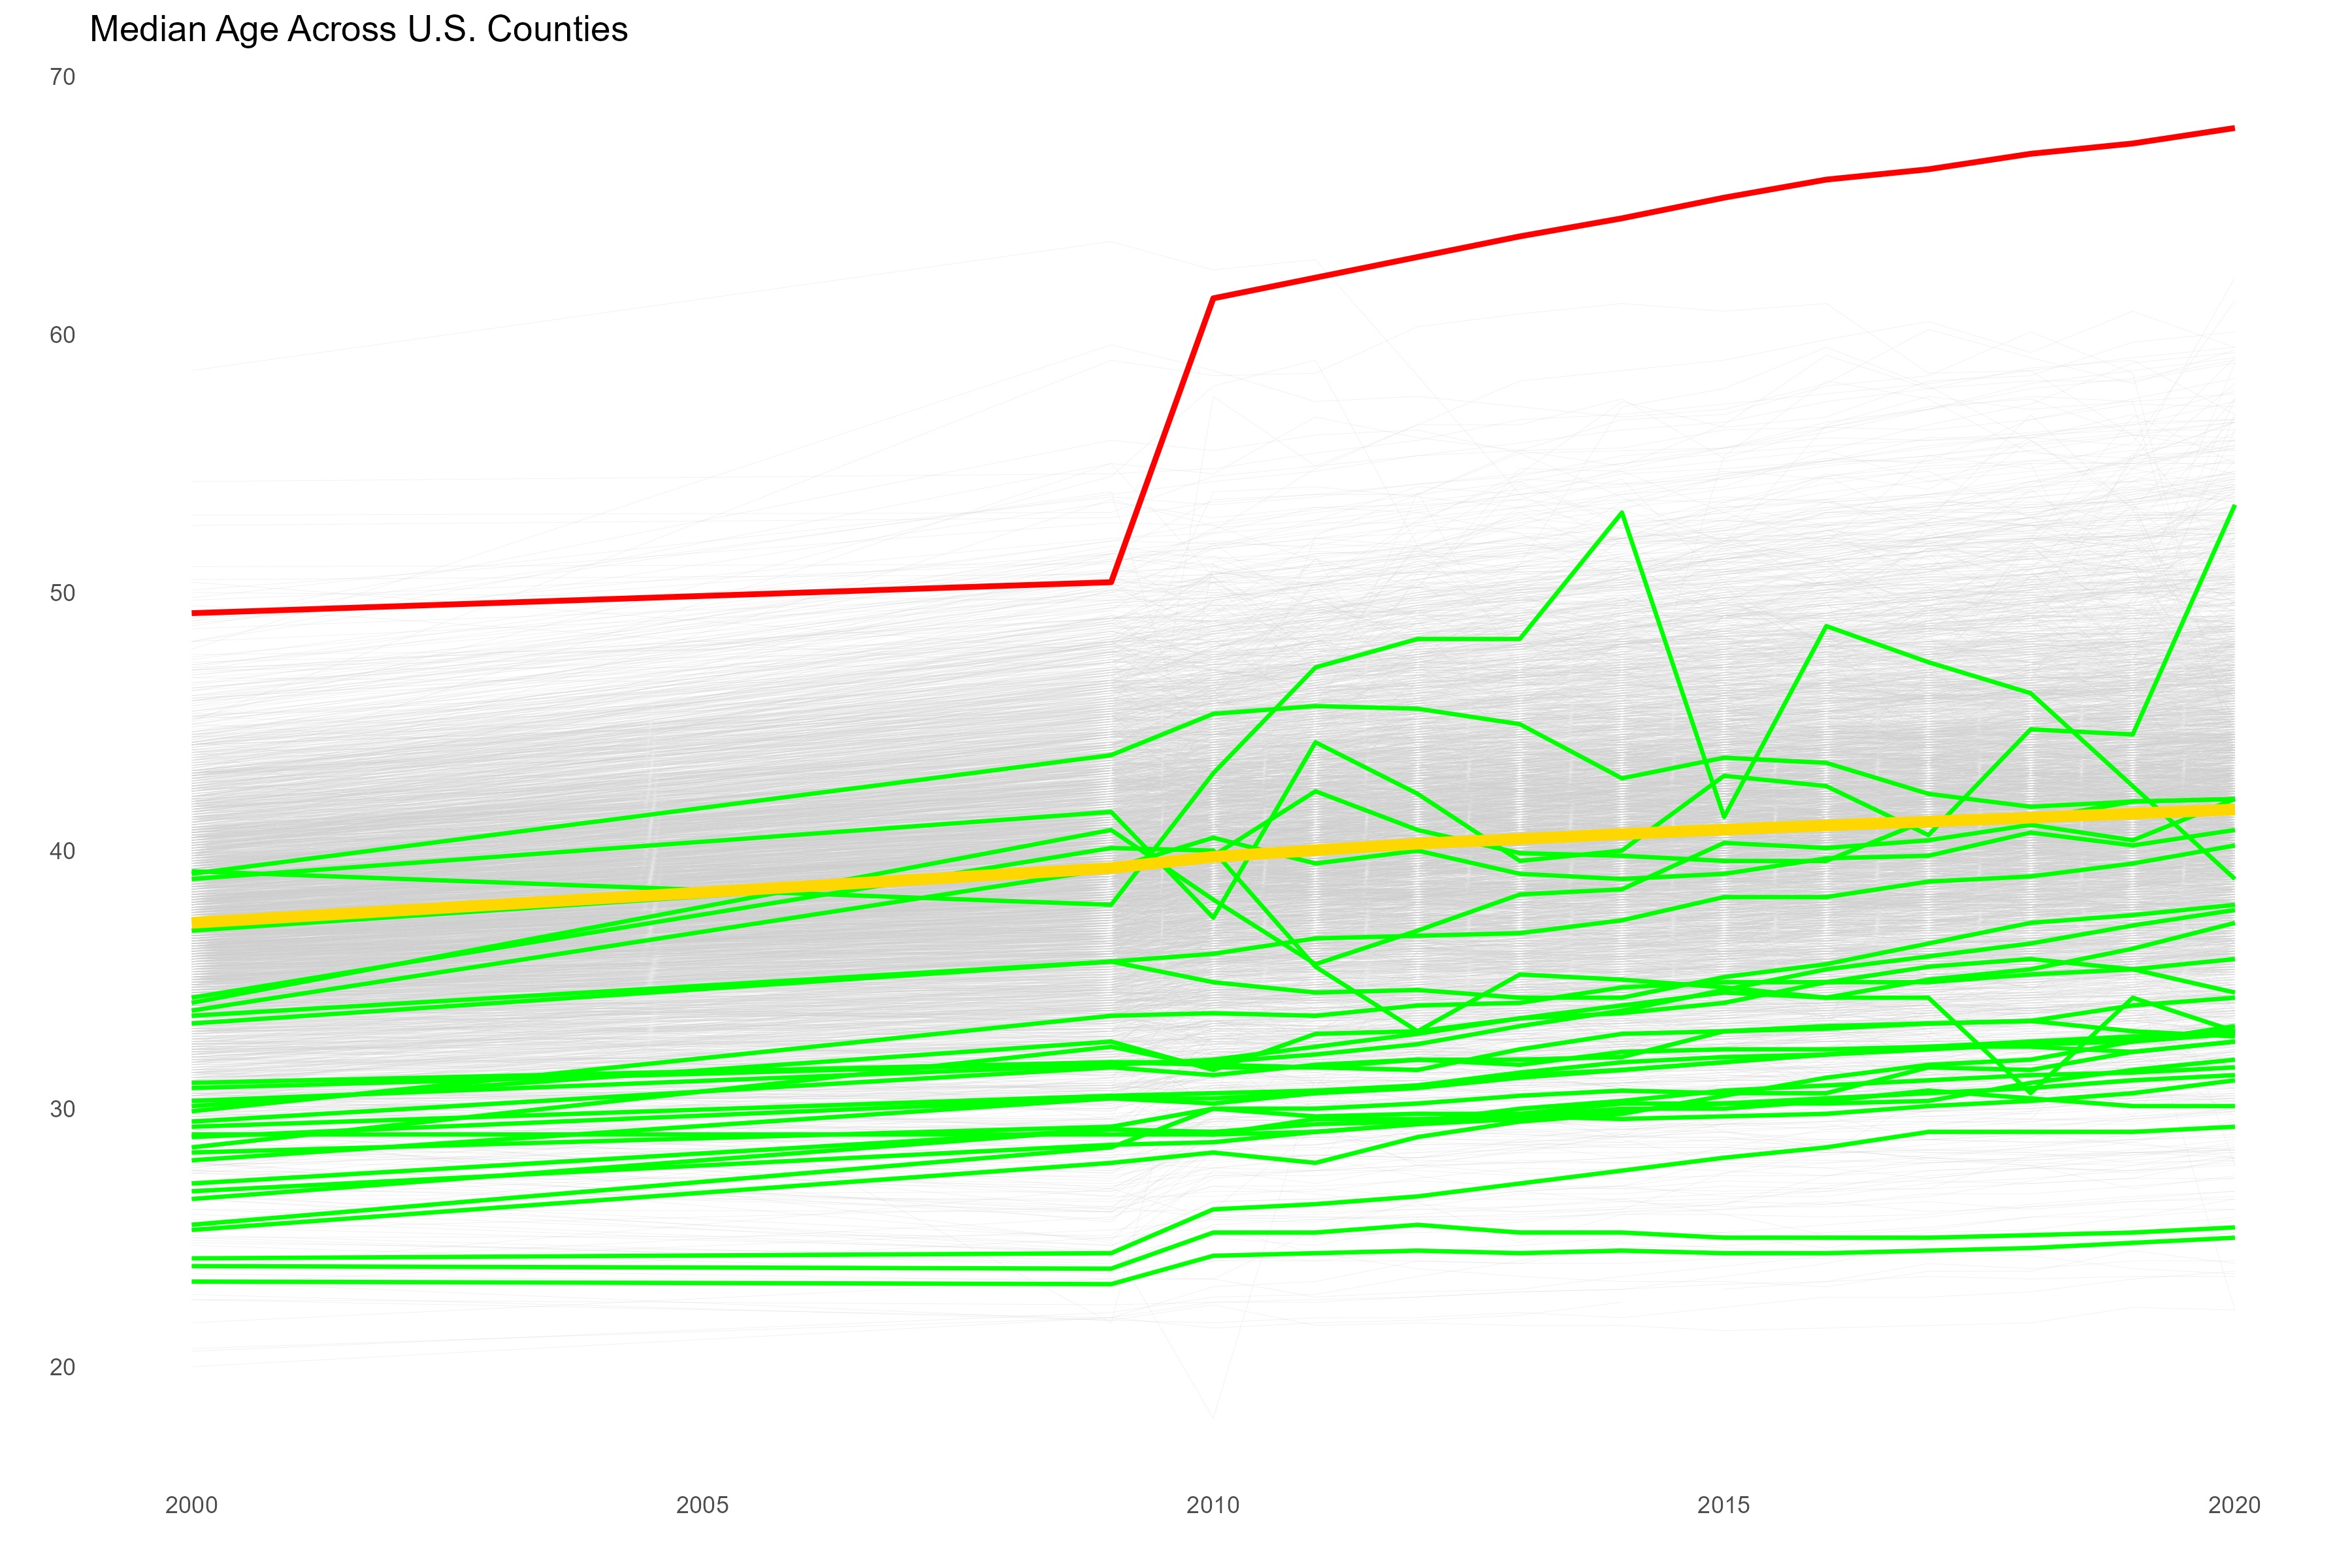
\includegraphics[width=0.75\textwidth,height=\textheight]{imgs/highlighted_spaghetti_plot_with_average_and_utah.png}

}

\caption{Guess which lines belongs to which county?}

\end{figure}

\hypertarget{proportion-of-60}{%
\section{Proportion of 60+}\label{proportion-of-60}}

\begin{itemize}
\tightlist
\item
  issues around health care provision
\item
  age related diseases (cognitive decline, Parkinson,\ldots)
\end{itemize}

\begin{figure}

{\centering 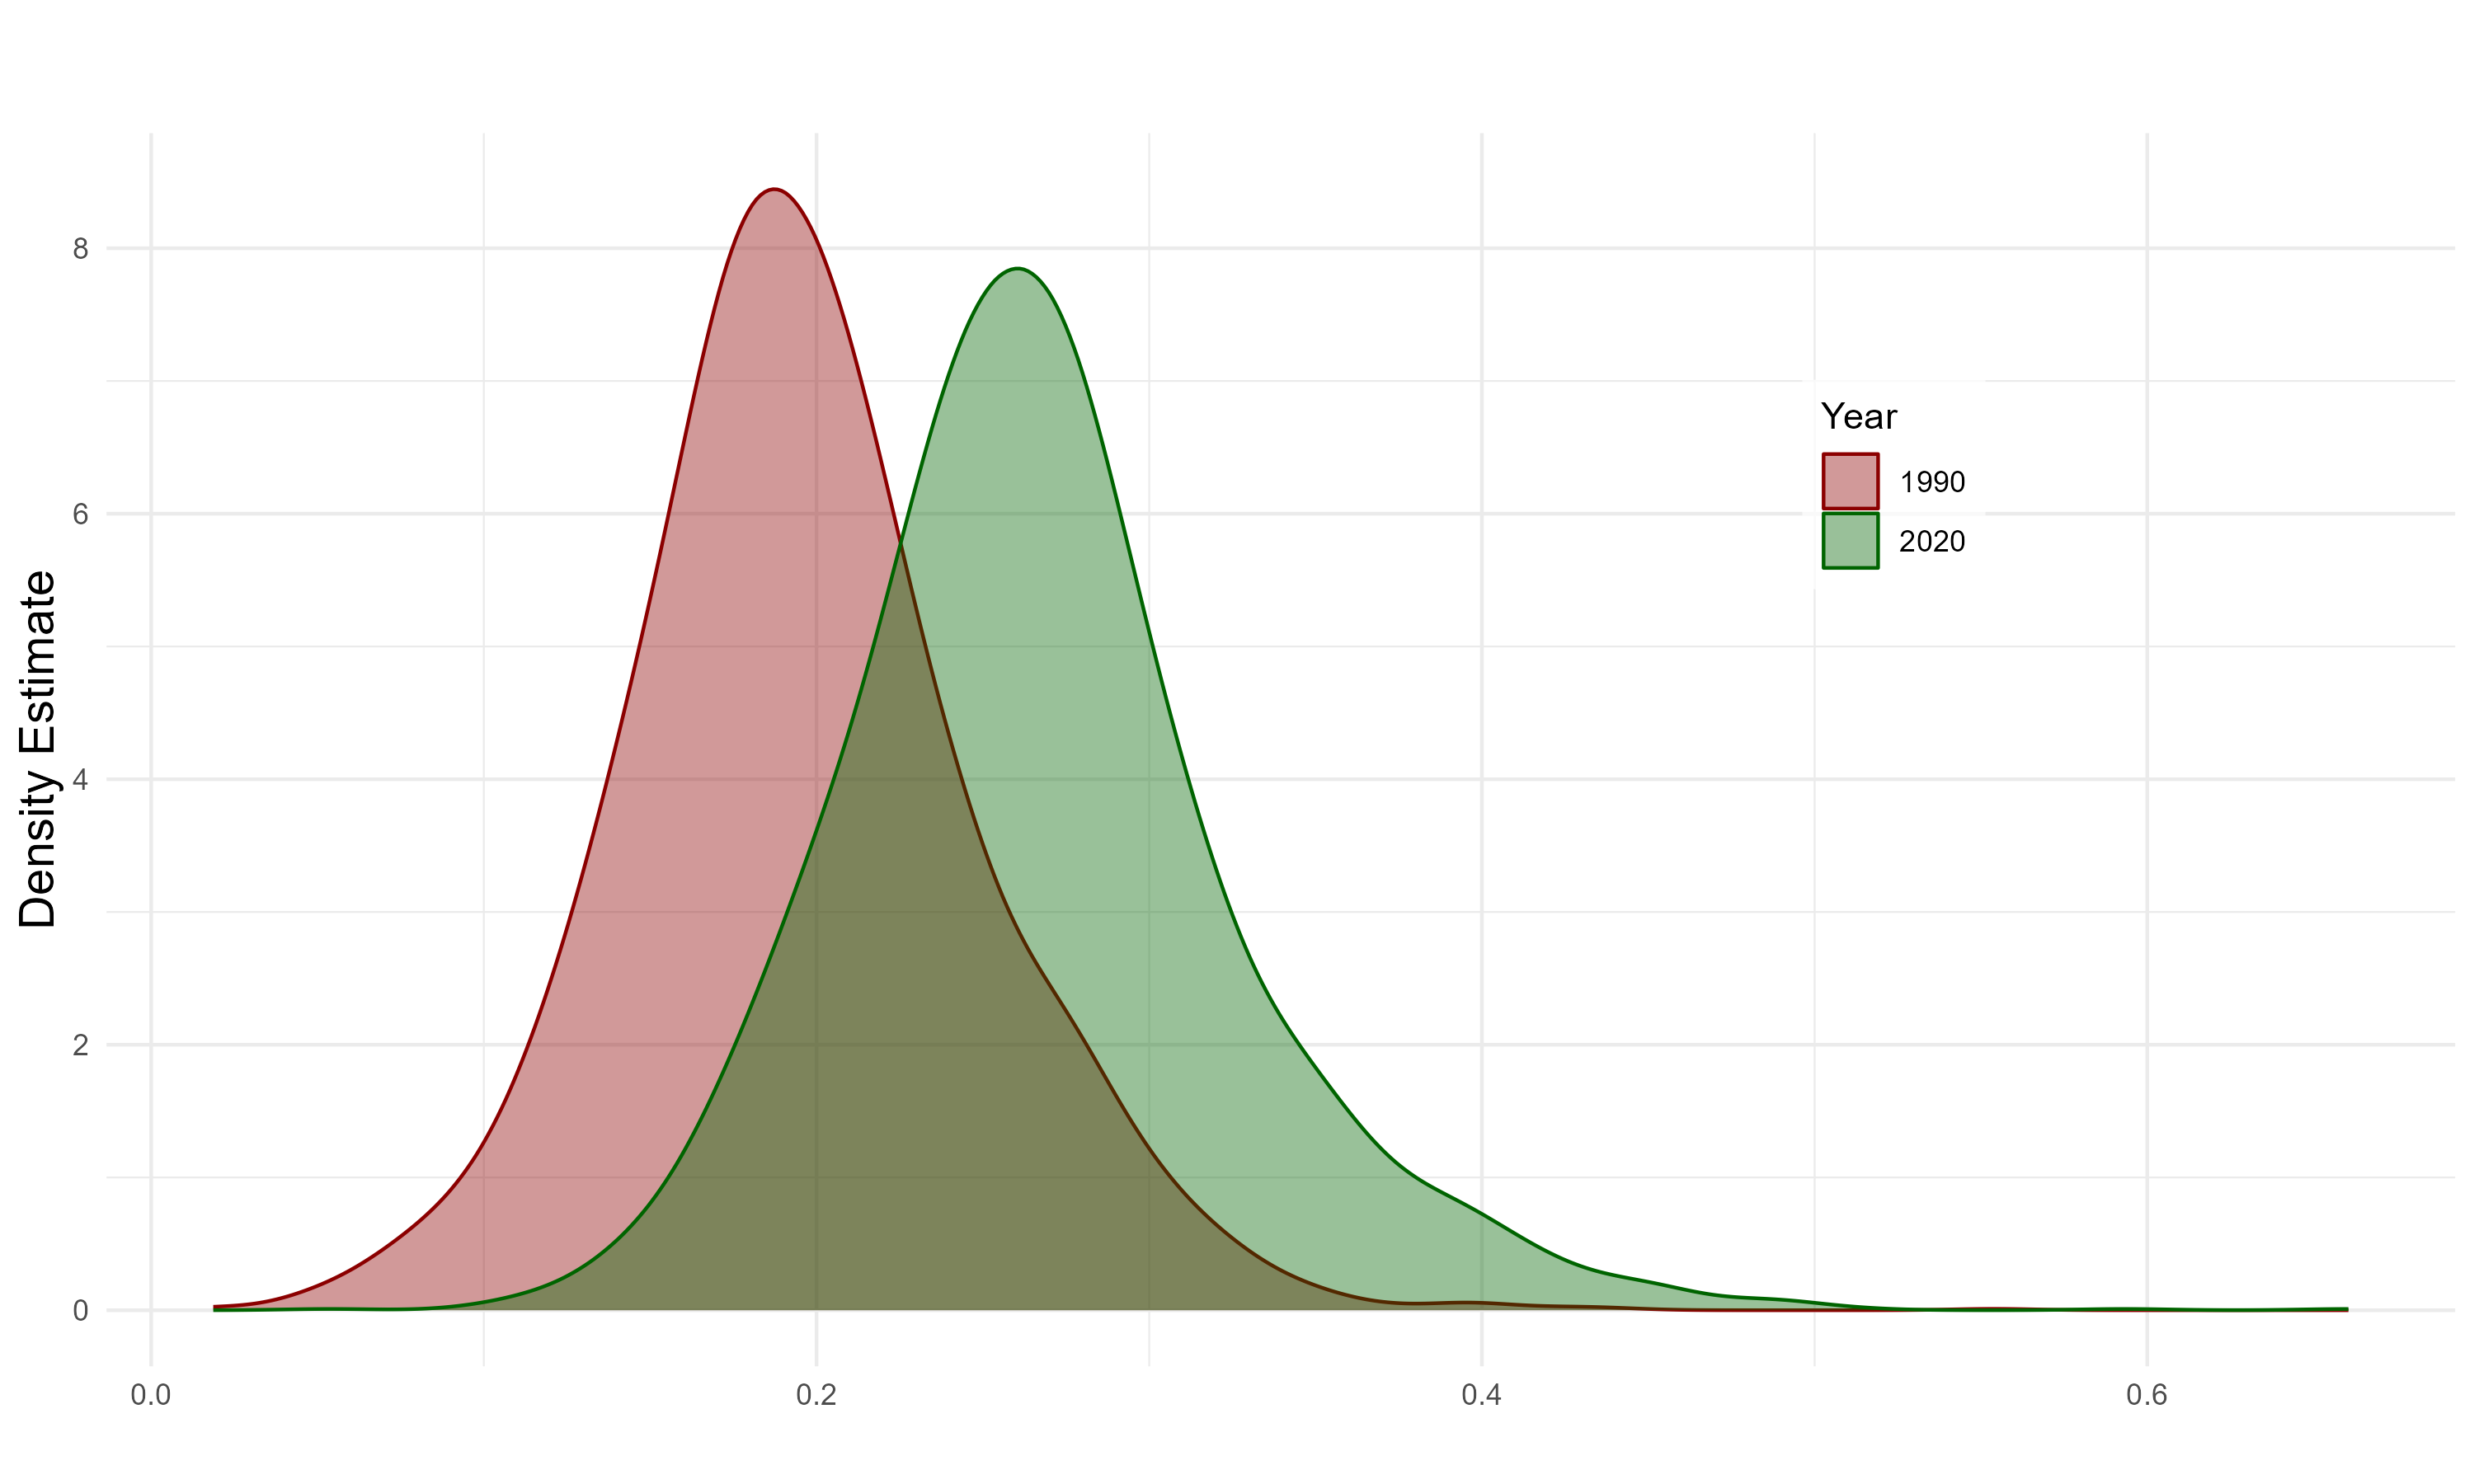
\includegraphics[width=0.6\textwidth,height=\textheight]{imgs/ksdensity_60plus_comparison.png}

}

\caption{Proportion of the Population 60+}

\end{figure}

\hypertarget{interesting-geographic-trends}{%
\section{Interesting geographic
trends}\label{interesting-geographic-trends}}

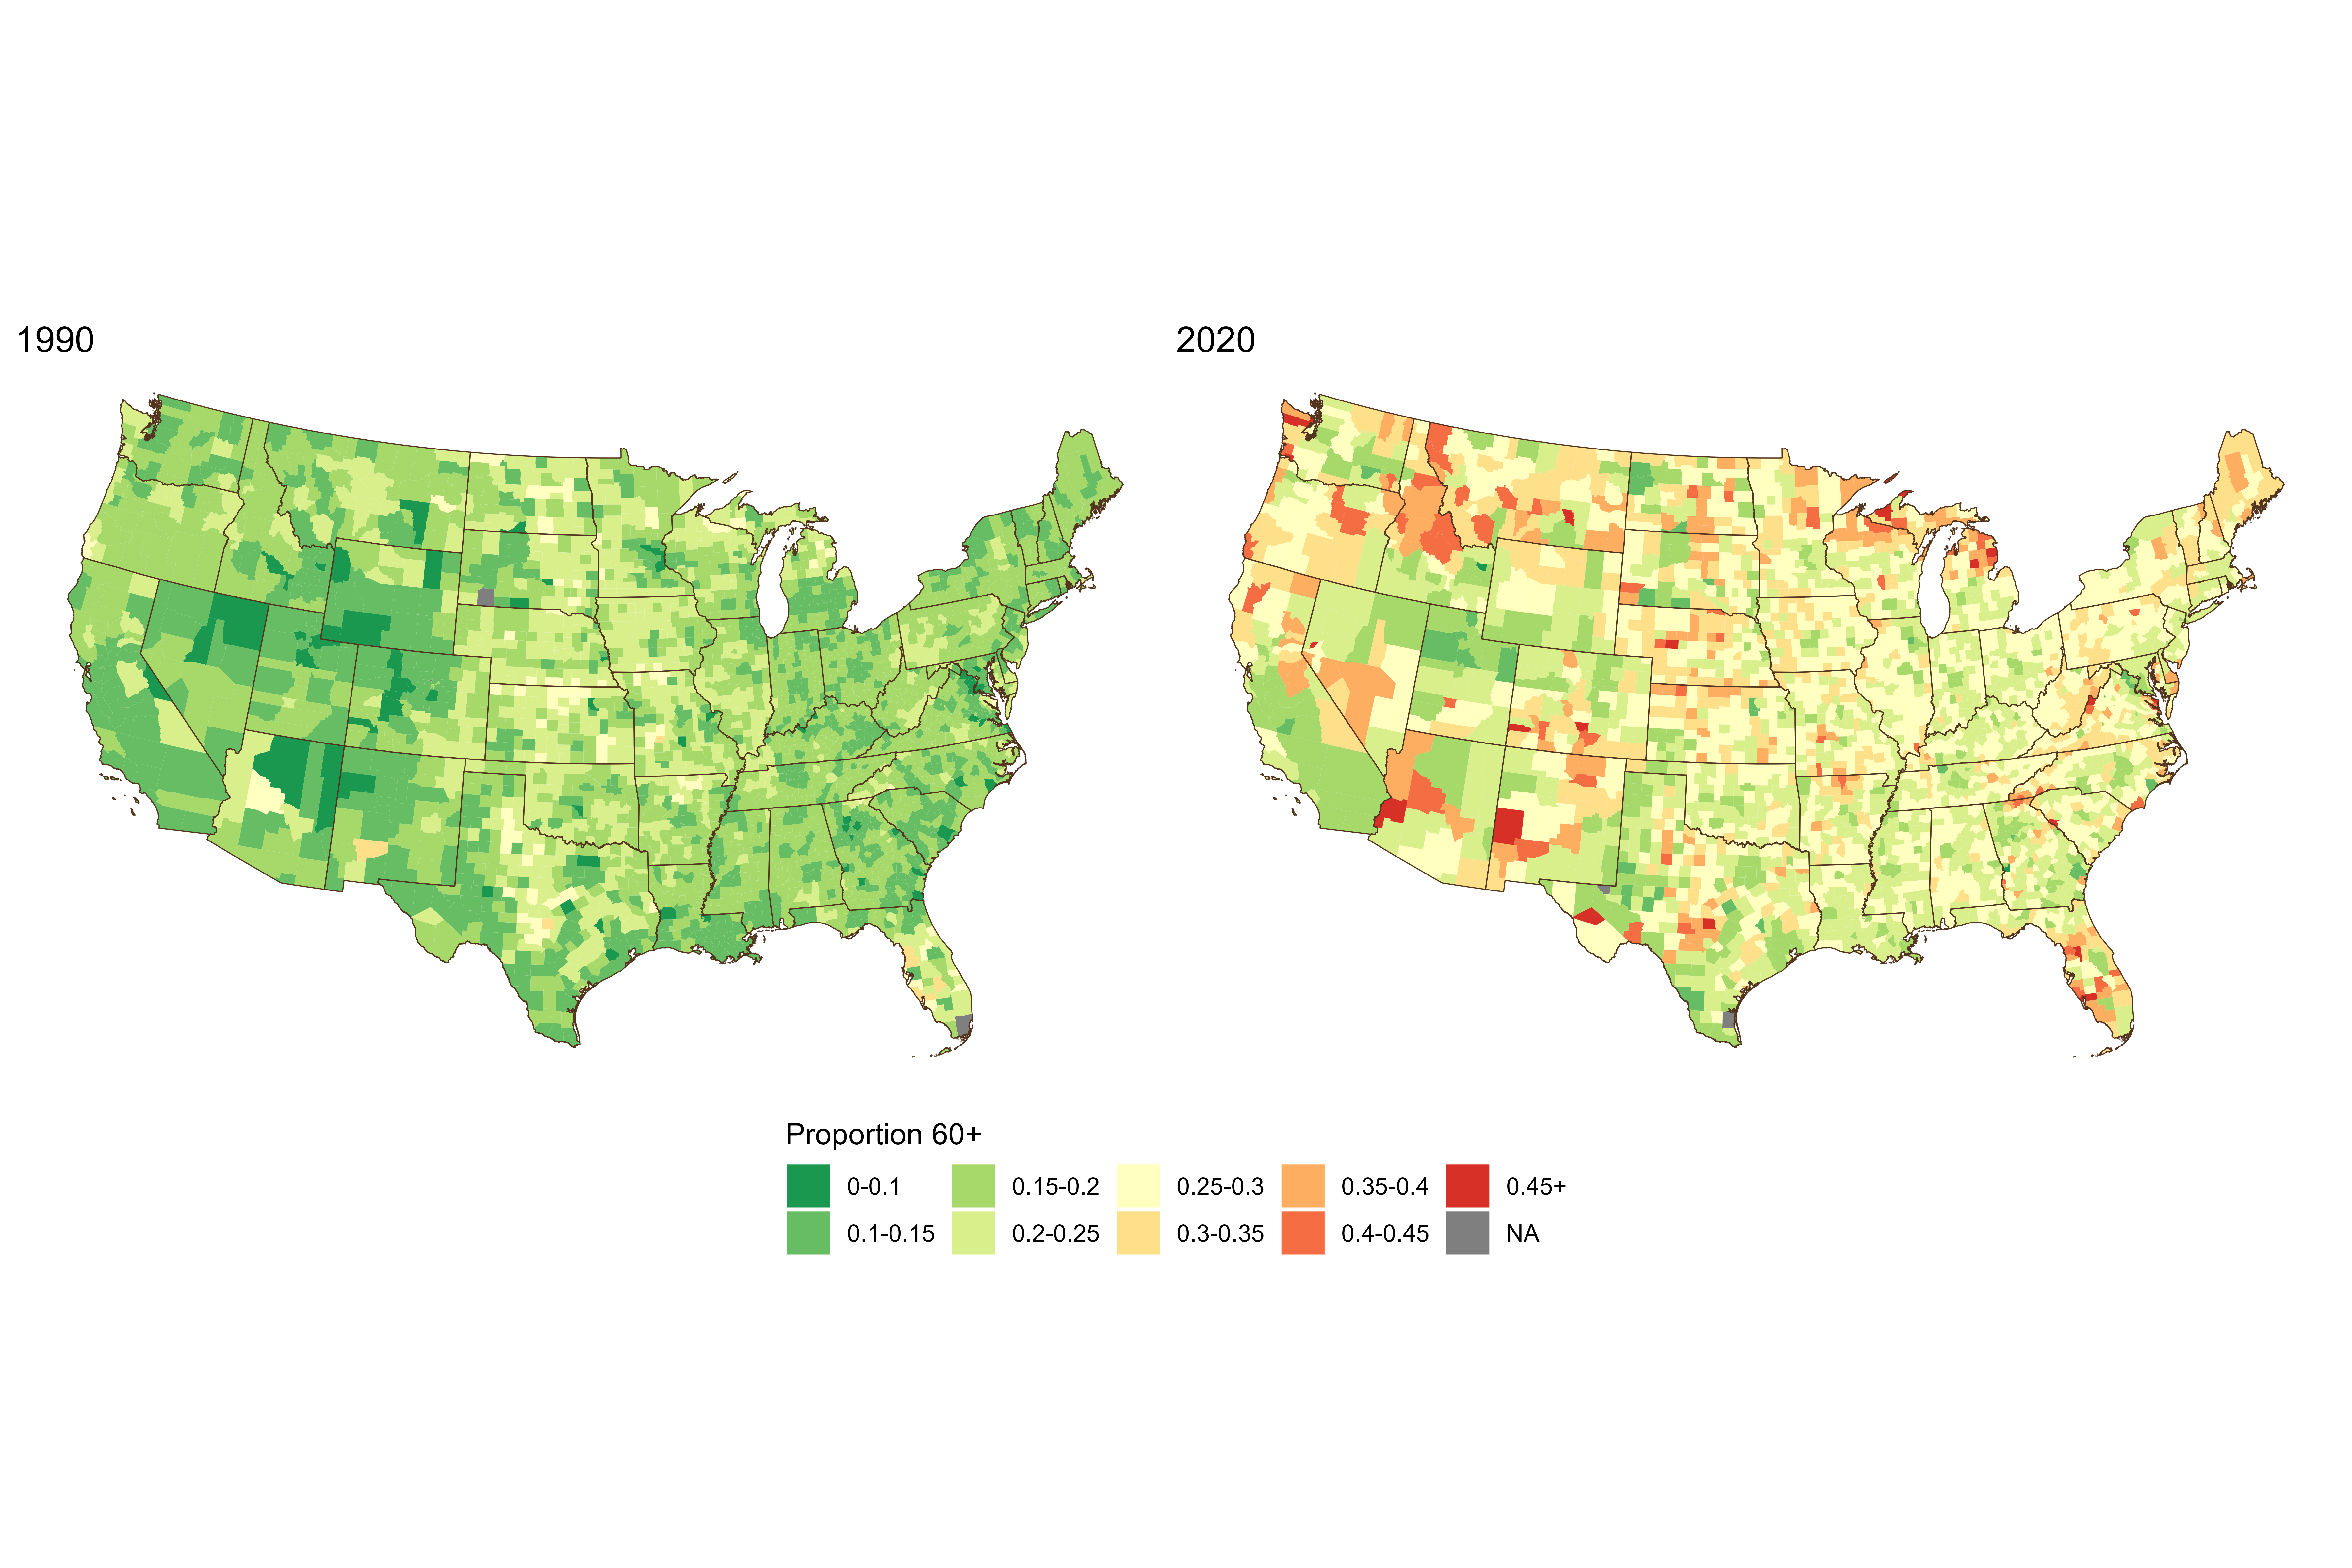
\includegraphics[width=0.98\textwidth,height=\textheight]{imgs/combined60propB.png}

\hypertarget{aim-1-of-the-grant}{%
\section{Aim 1 of the grant}\label{aim-1-of-the-grant}}

{ - \textbf{{[}`\ldots characterize change in neighborhood social \&
build environment variables relevant to cognition\ldots{}'{]}}}

\begin{itemize}
\tightlist
\item
  \textbf{Physical} function
\item
  \textbf{cognitive} function
\item
  ability to \textbf{age} in place
\end{itemize}

\hypertarget{characterize-social-and-built-environment-13}{%
\section{Characterize (social and built environment)
(1/3)}\label{characterize-social-and-built-environment-13}}

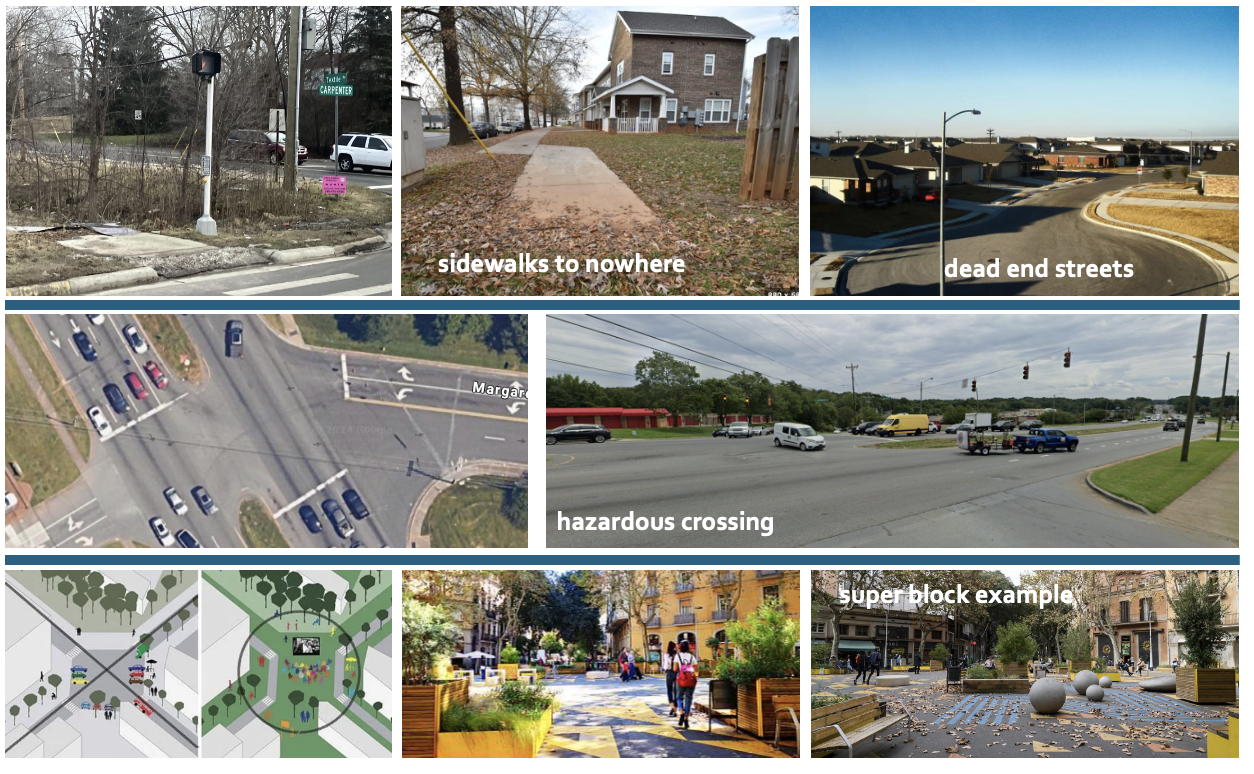
\includegraphics[width=0.8\textwidth,height=\textheight]{imgs/connectedNeighborhoodsB.png}

\hypertarget{characterize-social-and-built-environment-23}{%
\section{Characterize (social and built environment)
(2/3)}\label{characterize-social-and-built-environment-23}}

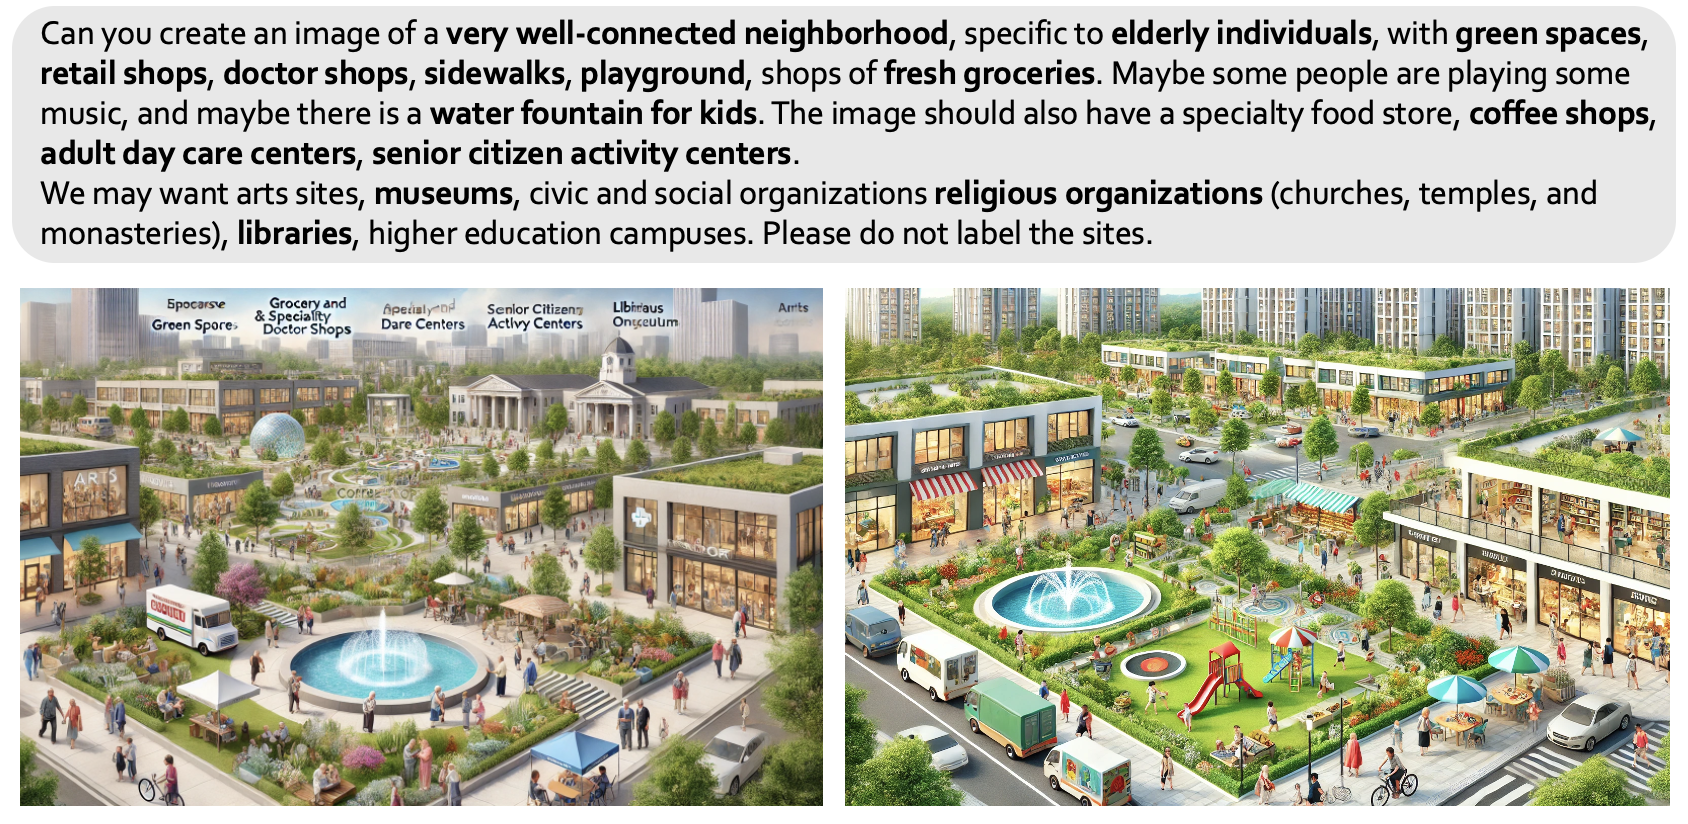
\includegraphics[width=0.7\textwidth,height=\textheight]{imgs/connectedNeighborhoodsC.png}

\hypertarget{characterize-social-and-built-environment-33}{%
\section{Characterize (social and built environment)
(3/3)}\label{characterize-social-and-built-environment-33}}

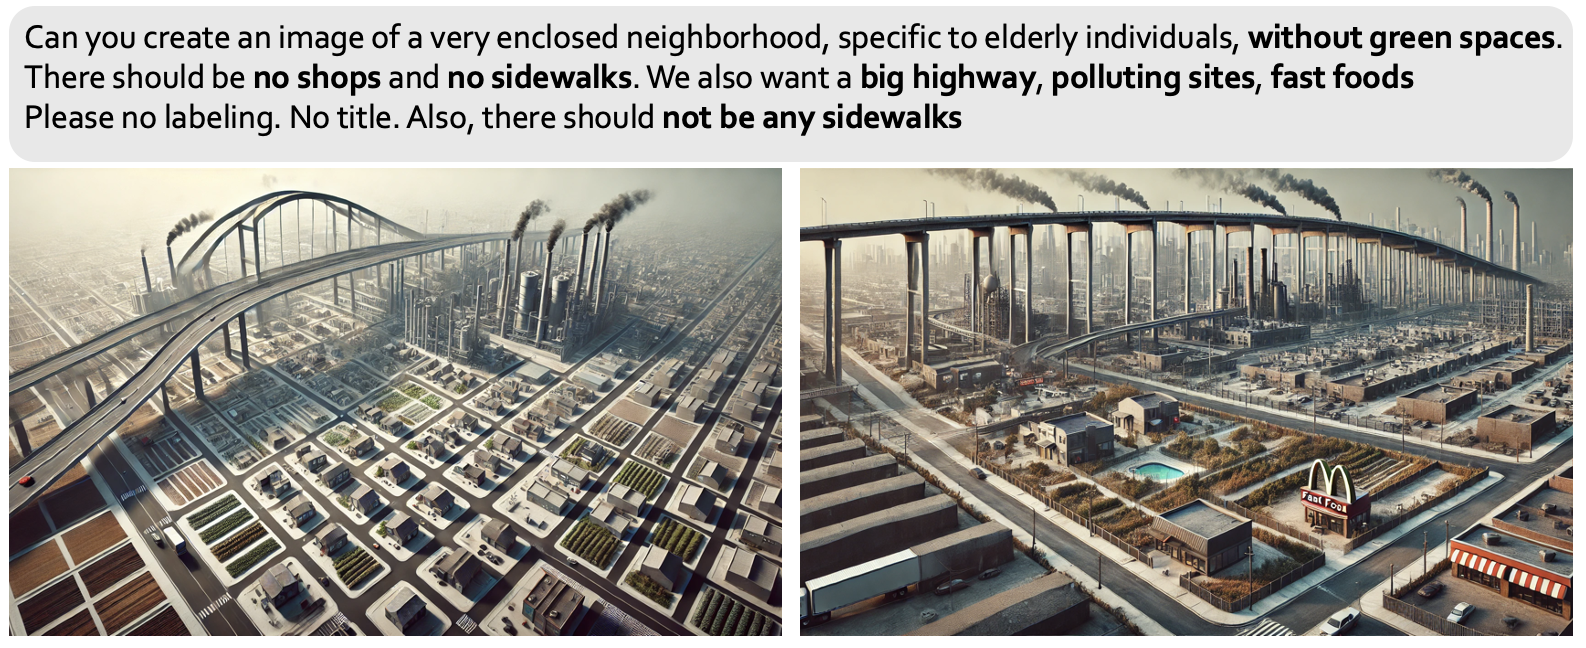
\includegraphics[width=0.7\textwidth,height=\textheight]{imgs/connectedNeighborhoodsD.png}

\hypertarget{research-questions}{%
\section{Research questions?}\label{research-questions}}

\begin{itemize}
\tightlist
\item
  How can we characterize age-friendly communities?
\item
  Are there distinct \textbf{clusters} of neighborhood aging resources?

  \begin{itemize}
  \tightlist
  \item
    Have the resources within \textbf{clusters} changed over time, and
    how?
  \end{itemize}
\item
  Our data reflect three domains:

  \begin{itemize}
  \tightlist
  \item
    \textbf{physical} function, \textbf{cognitive} function, ability to
    \textbf{age} in place
  \end{itemize}
\end{itemize}

\hypertarget{our-approach---reproducible-in-r}{%
\section{\texorpdfstring{Our approach - reproducible in
\texttt{R}}{Our approach - reproducible in R}}\label{our-approach---reproducible-in-r}}

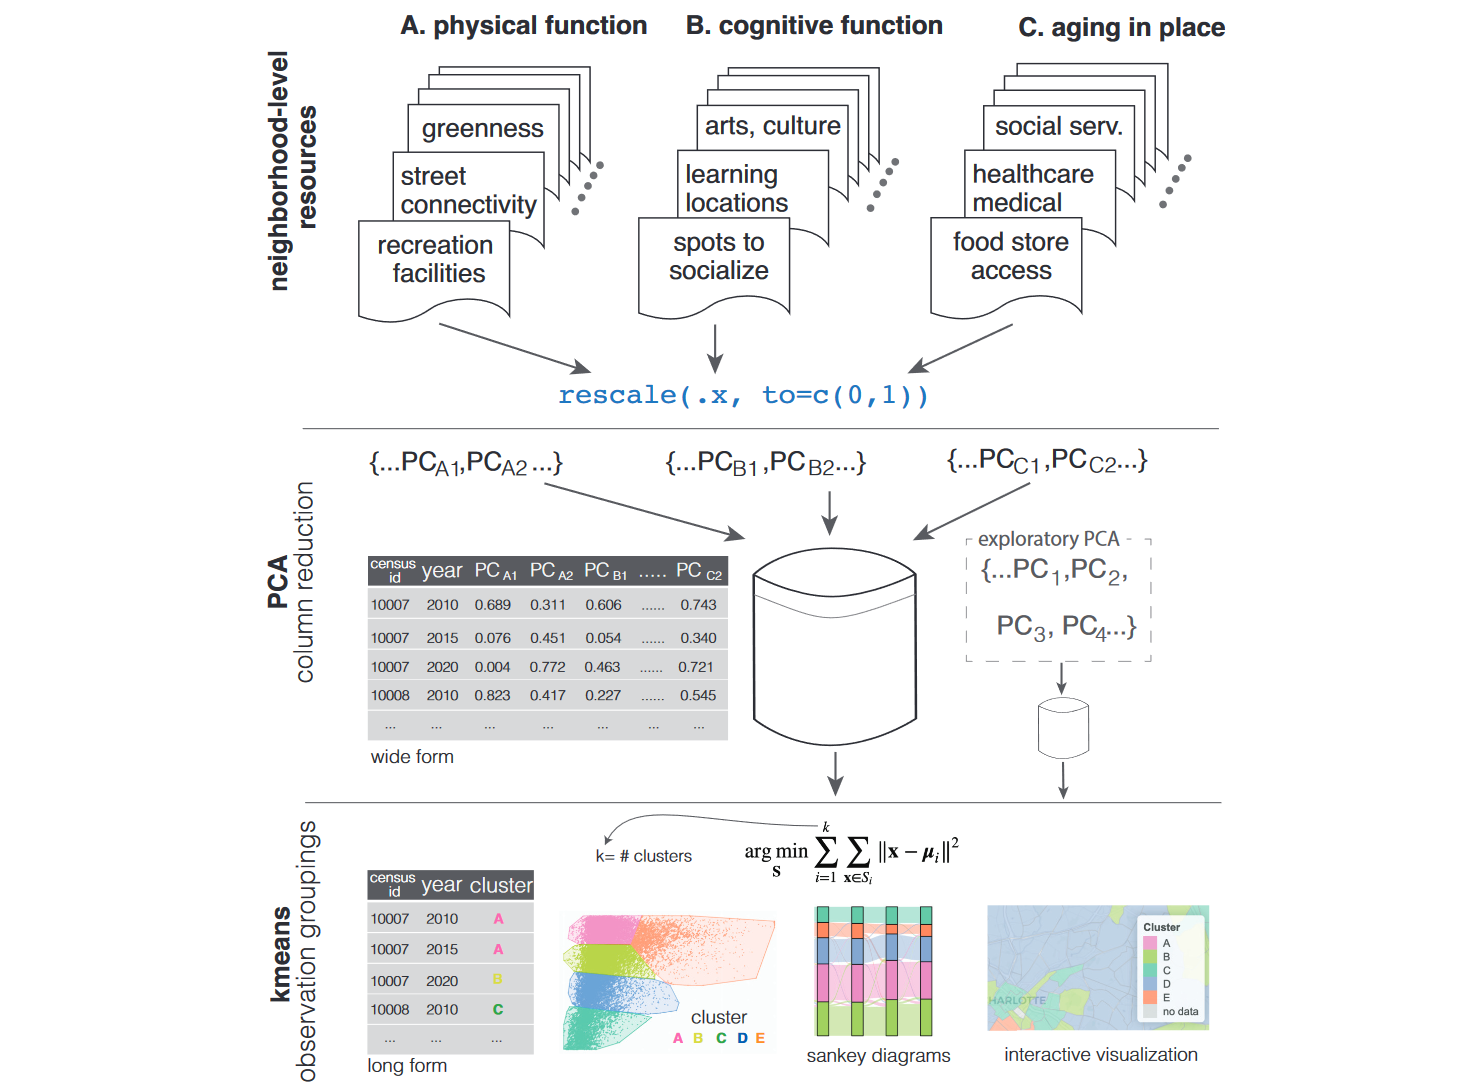
\includegraphics[width=0.9\textwidth,height=\textheight]{imgs/process.png}

\hypertarget{dataset}{%
\section{Dataset:}\label{dataset}}

\begin{itemize}
\tightlist
\item
  \textbf{Yearly observations} for each census tract {[}1990-2022{]}
\item
  72,246 tracts * 33 y. * 19 var. = 45,298,242 measurements
\end{itemize}

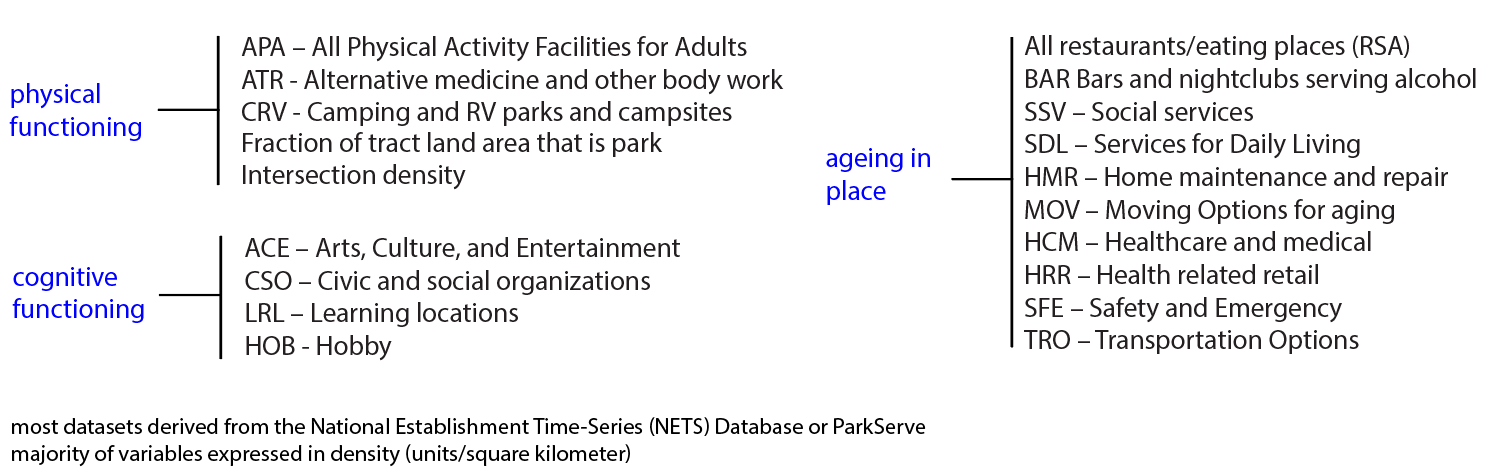
\includegraphics[width=0.9\textwidth,height=\textheight]{imgs/datasets.png}

\hypertarget{example-of-a-variable-apa}{%
\section{Example of a Variable (APA):}\label{example-of-a-variable-apa}}

\begin{figure}

{\centering 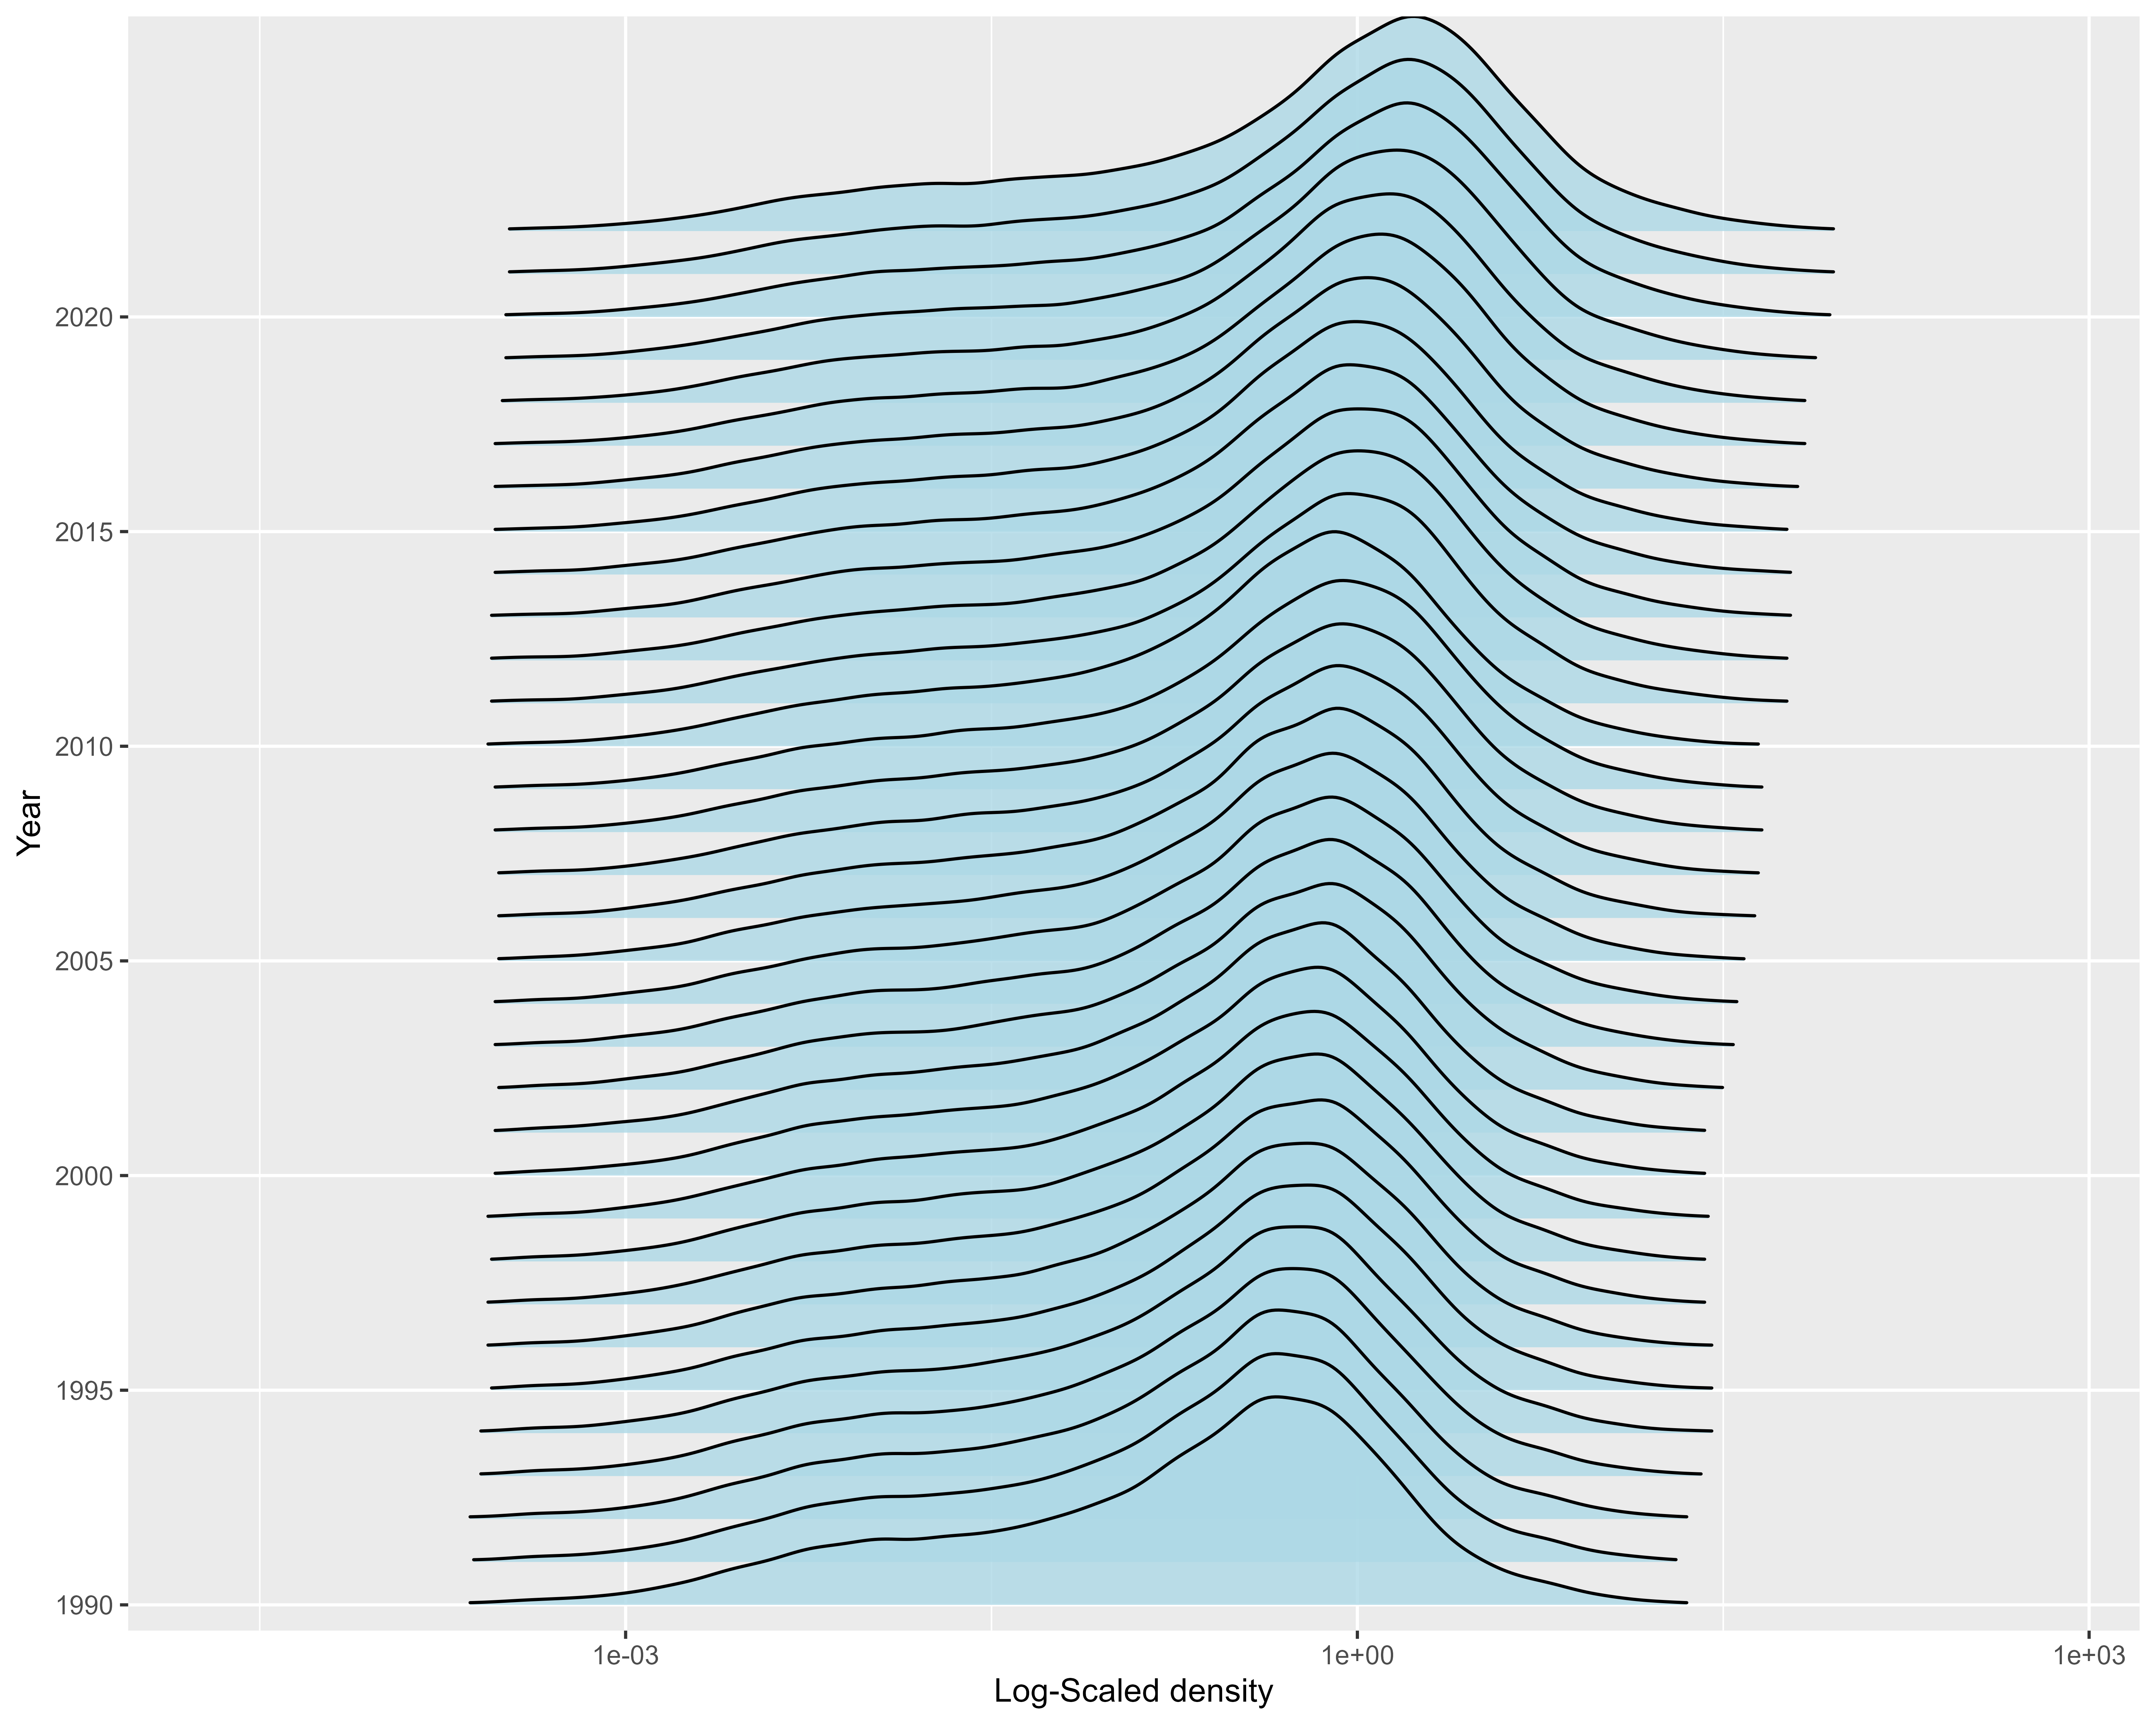
\includegraphics[width=0.6\textwidth,height=\textheight]{imgs/ggridge_histogram_apa_log.png}

}

\caption{Distribution of All Physical Activity Facilities for Adults
(APA) by Year}

\end{figure}

\hypertarget{example-of-a-variable-apa-1}{%
\section{Example of a Variable
(APA):}\label{example-of-a-variable-apa-1}}

\begin{figure}

{\centering 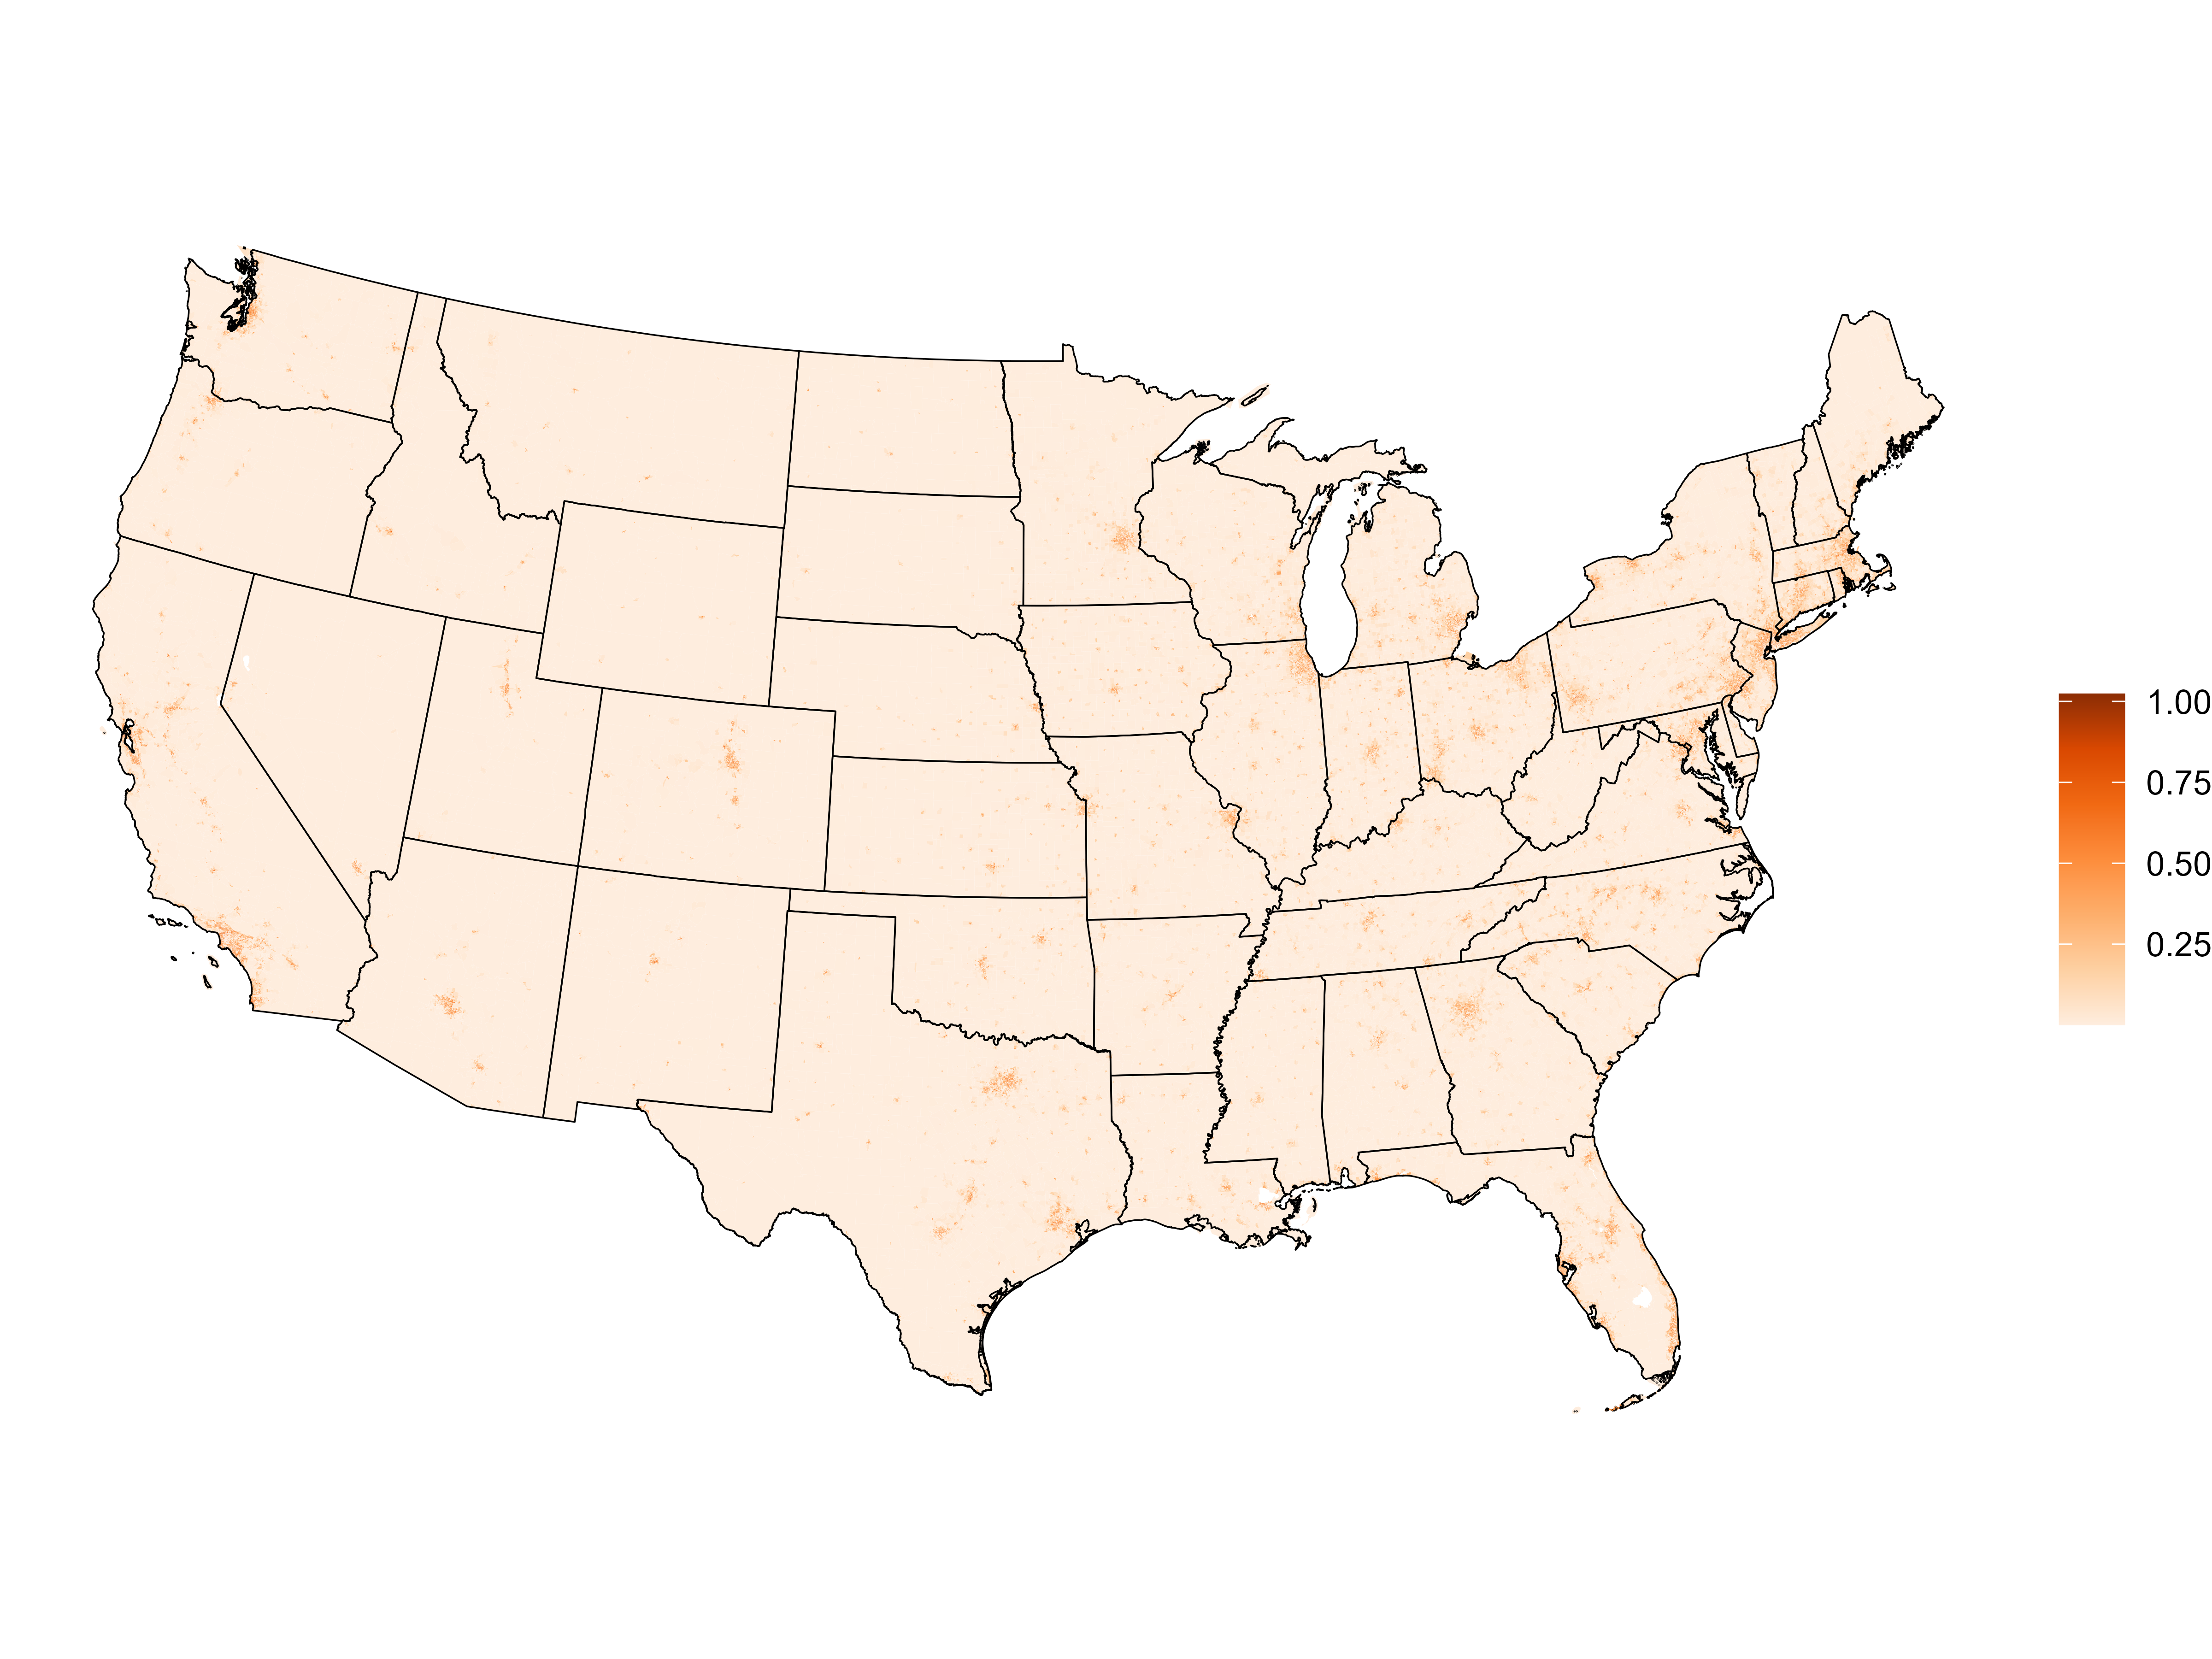
\includegraphics[width=0.7\textwidth,height=\textheight]{imgs/apa_2000.png}

}

\caption{Geographic Distribution of APA Facilities for Adults in 2000}

\end{figure}

\hypertarget{example-of-a-variable-park}{%
\section{Example of a Variable
(Park):}\label{example-of-a-variable-park}}

\begin{figure}

{\centering 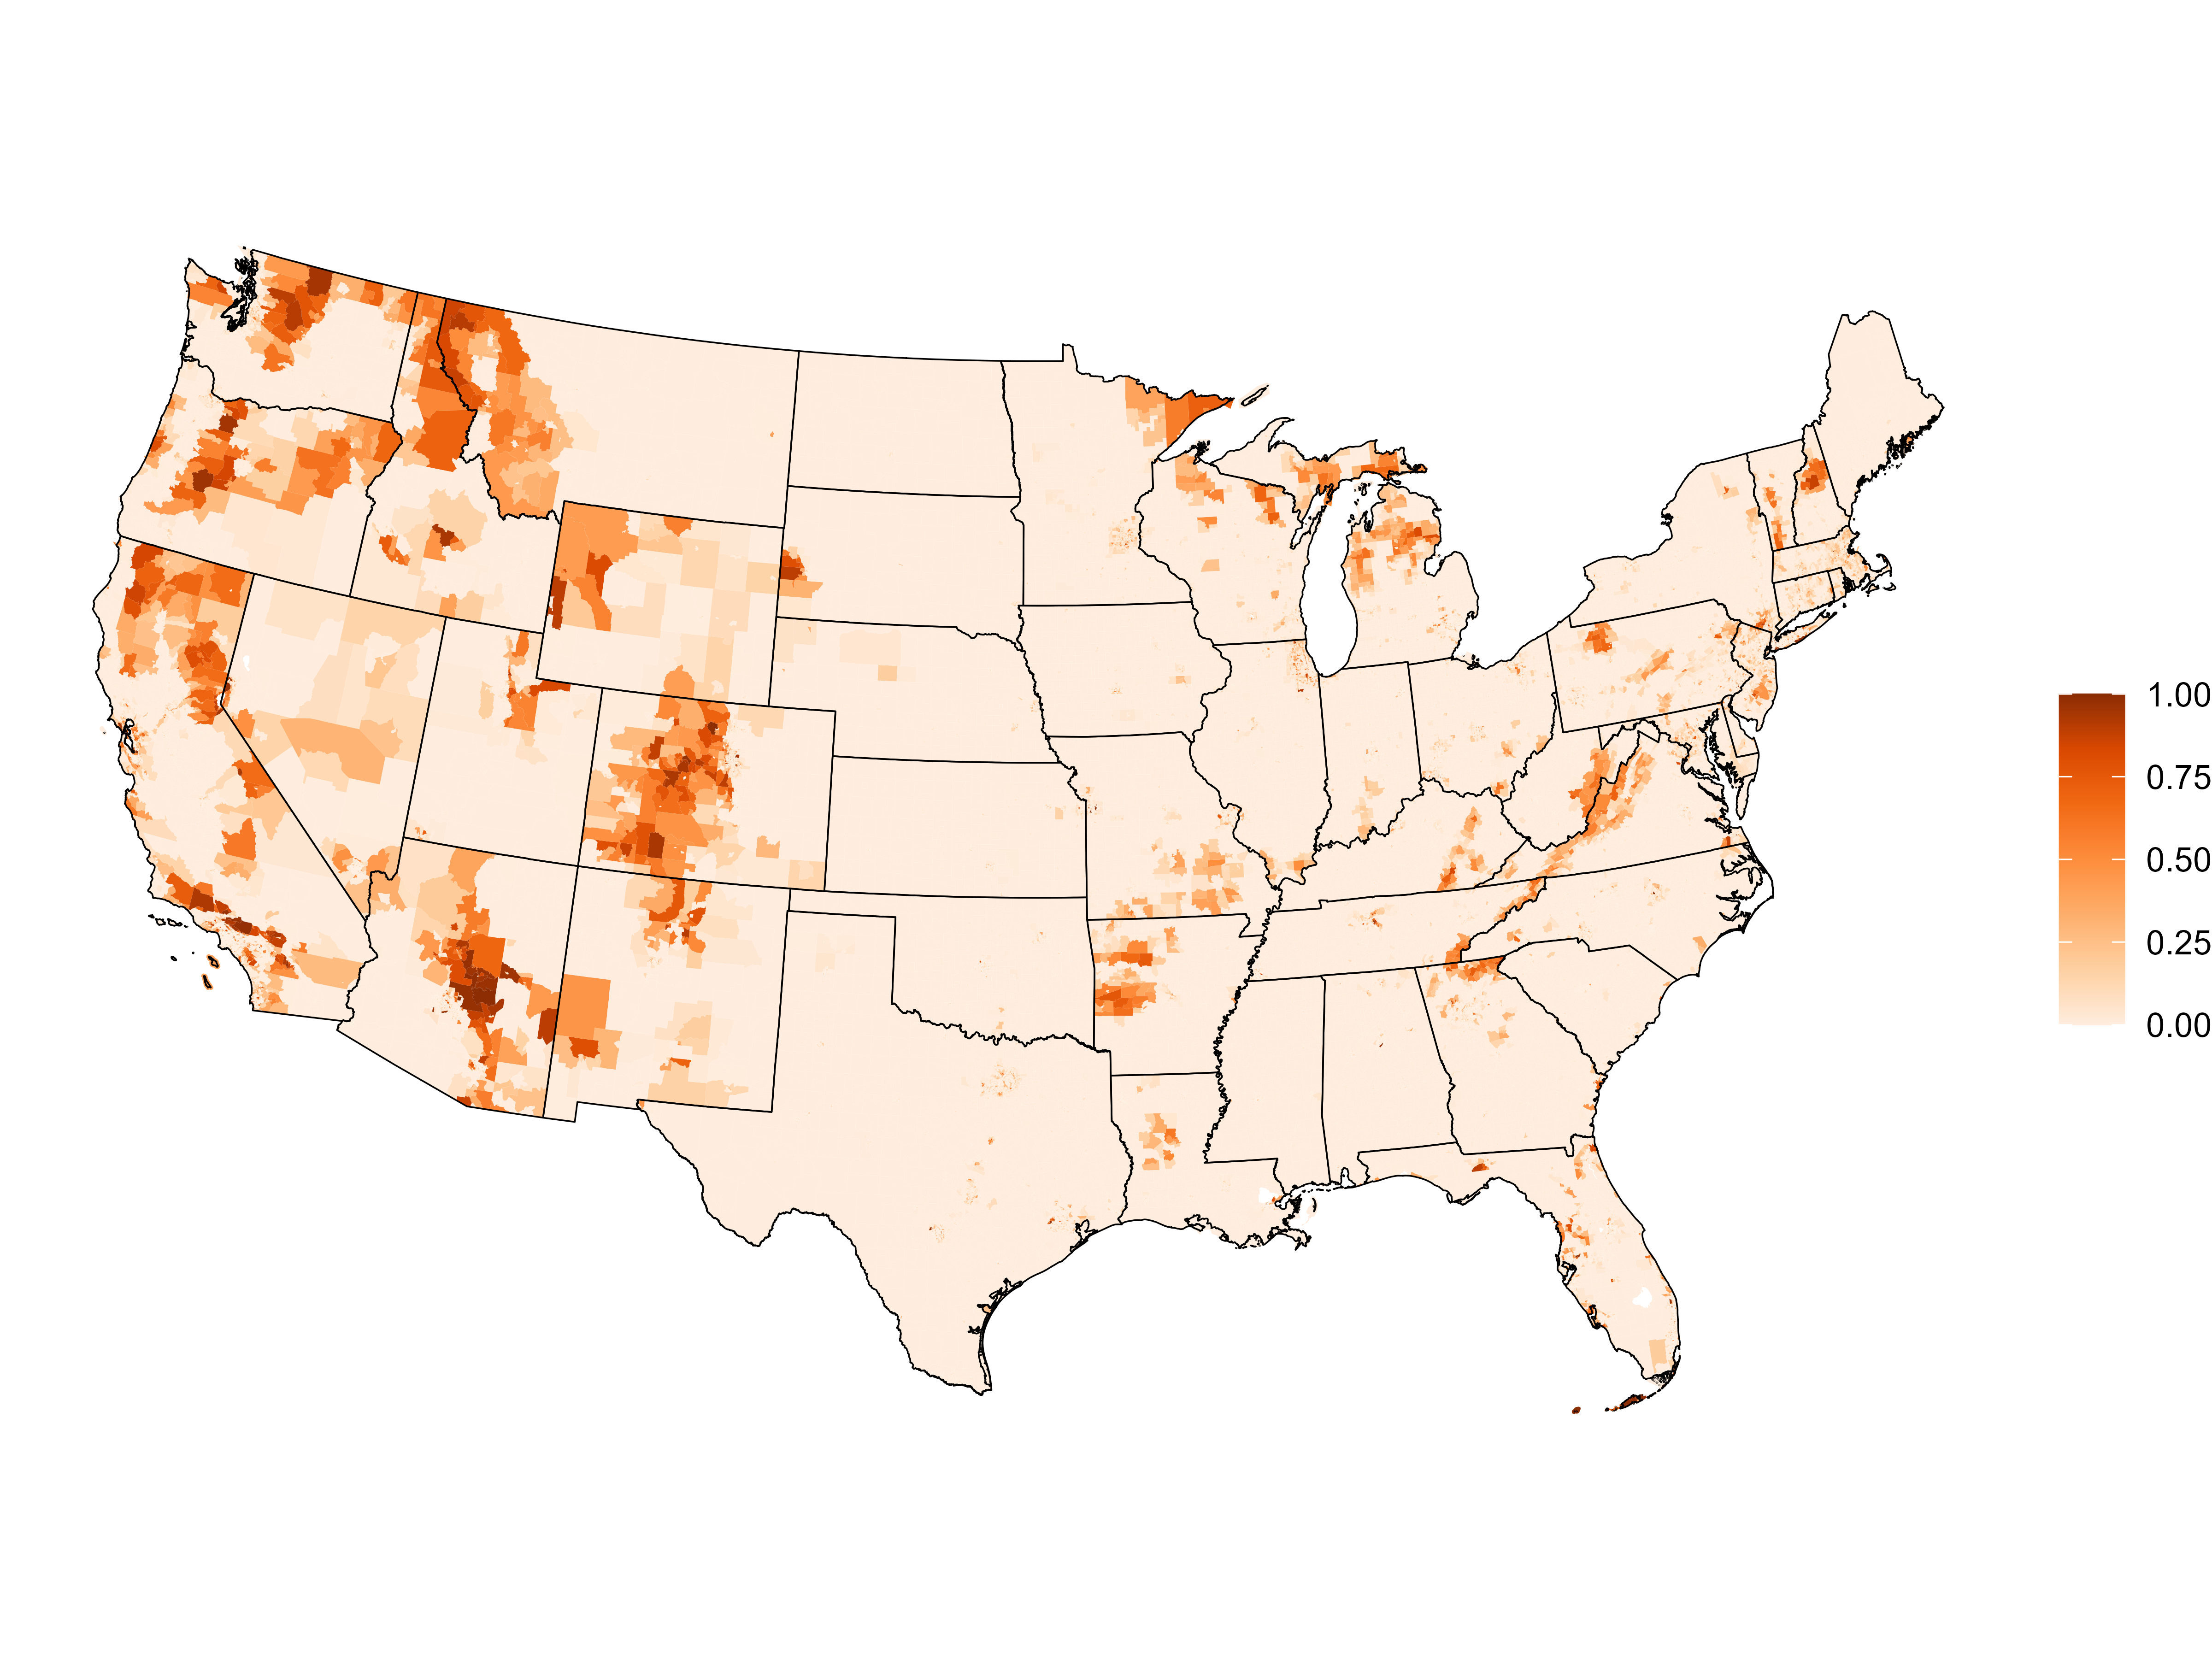
\includegraphics[width=0.7\textwidth,height=\textheight]{imgs/park_2000.png}

}

\caption{Fraction of park size (2000)}

\end{figure}

\hypertarget{correlation-among-variables}{%
\section{Correlation among
variables:}\label{correlation-among-variables}}

\begin{figure}

{\centering 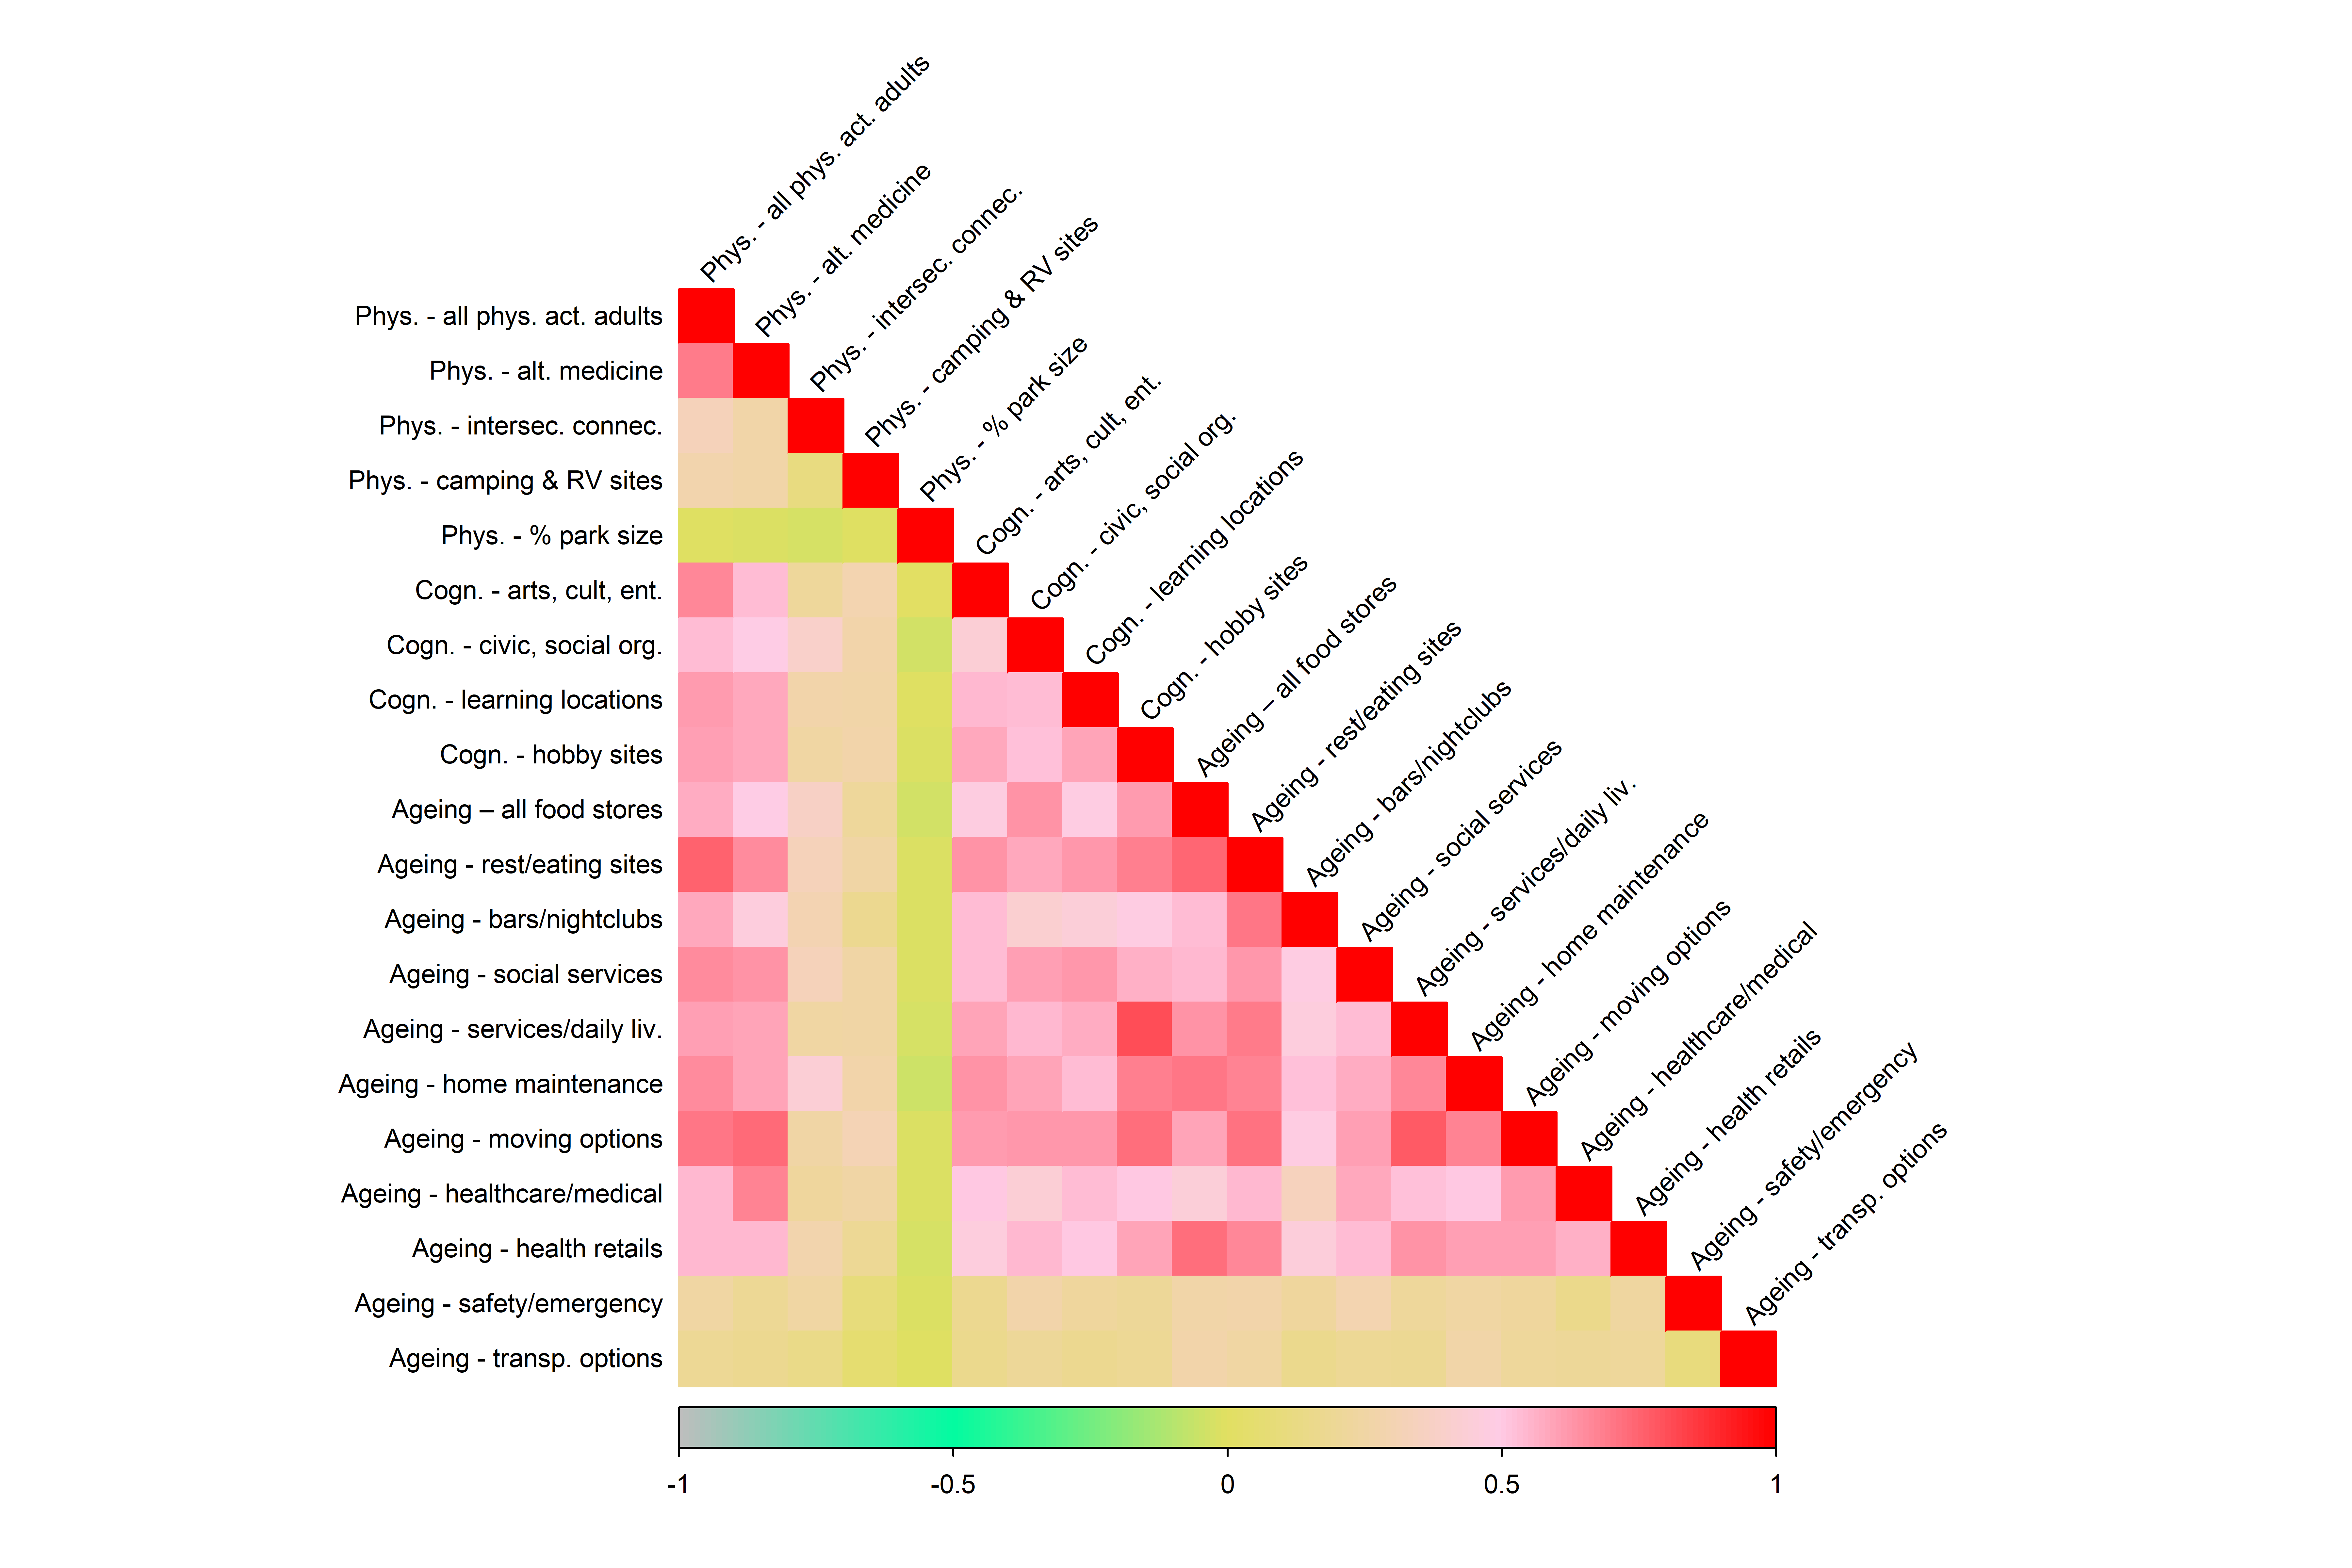
\includegraphics[width=0.7\textwidth,height=\textheight]{imgs/correlationPlot1.png}

}

\caption{Correlation among 19 variables considered in our study}

\end{figure}

\hypertarget{methods-pca-approach}{%
\section{\texorpdfstring{Methods: \texttt{PCA}
approach}{Methods: PCA approach}}\label{methods-pca-approach}}

\begin{itemize}
\tightlist
\item
  technique of dimensionality reduction
\item
  transforms a set of correlated variables into a smaller set of
  uncorrelated variables
\item
  these are called principal components, which should explain a large
  amount of variance from initial dataset
\item
  \textbf{domain}-driven PCA or \textbf{data}-driven PCA
\end{itemize}

\hypertarget{pca-results--physical-domain}{%
\section{PCA results -physical
domain:}\label{pca-results--physical-domain}}

\begin{figure}

{\centering 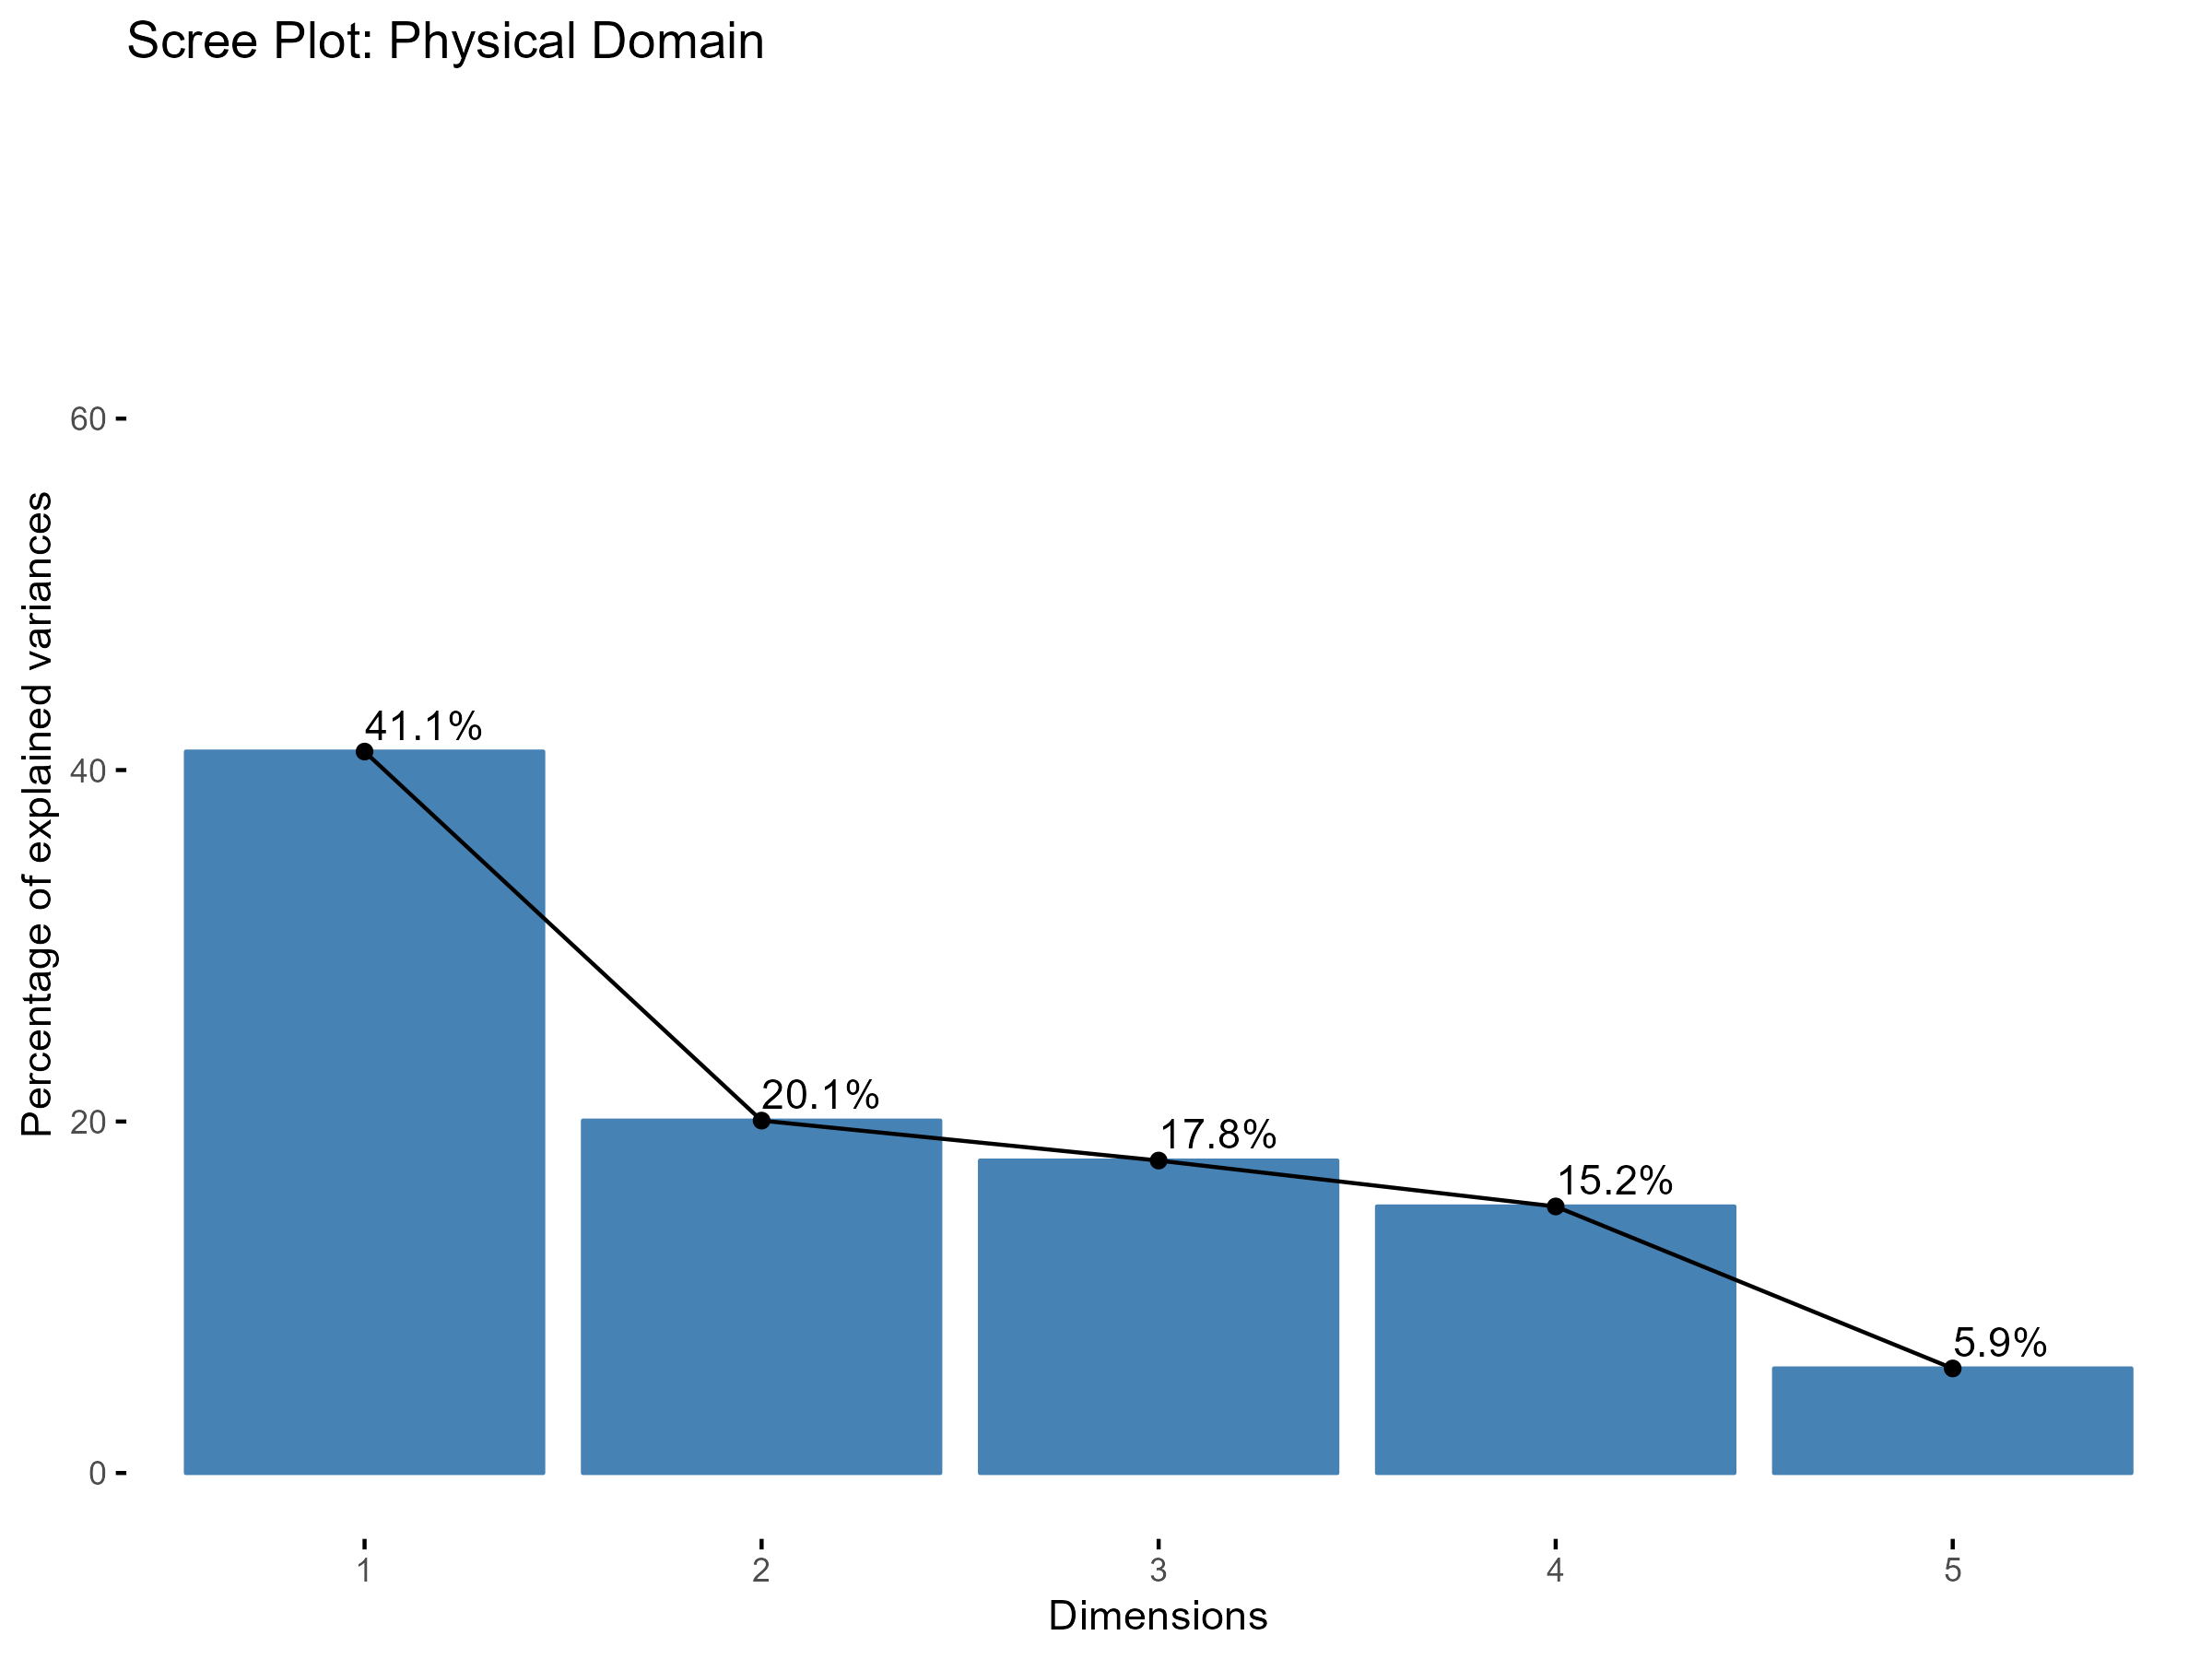
\includegraphics[width=0.7\textwidth,height=\textheight]{imgs/scree_plot_physical.png}

}

\caption{Scree plot for the physical domain}

\end{figure}

\hypertarget{pca-results--cognitive-domain}{%
\section{PCA results -Cognitive
domain:}\label{pca-results--cognitive-domain}}

\begin{figure}

{\centering 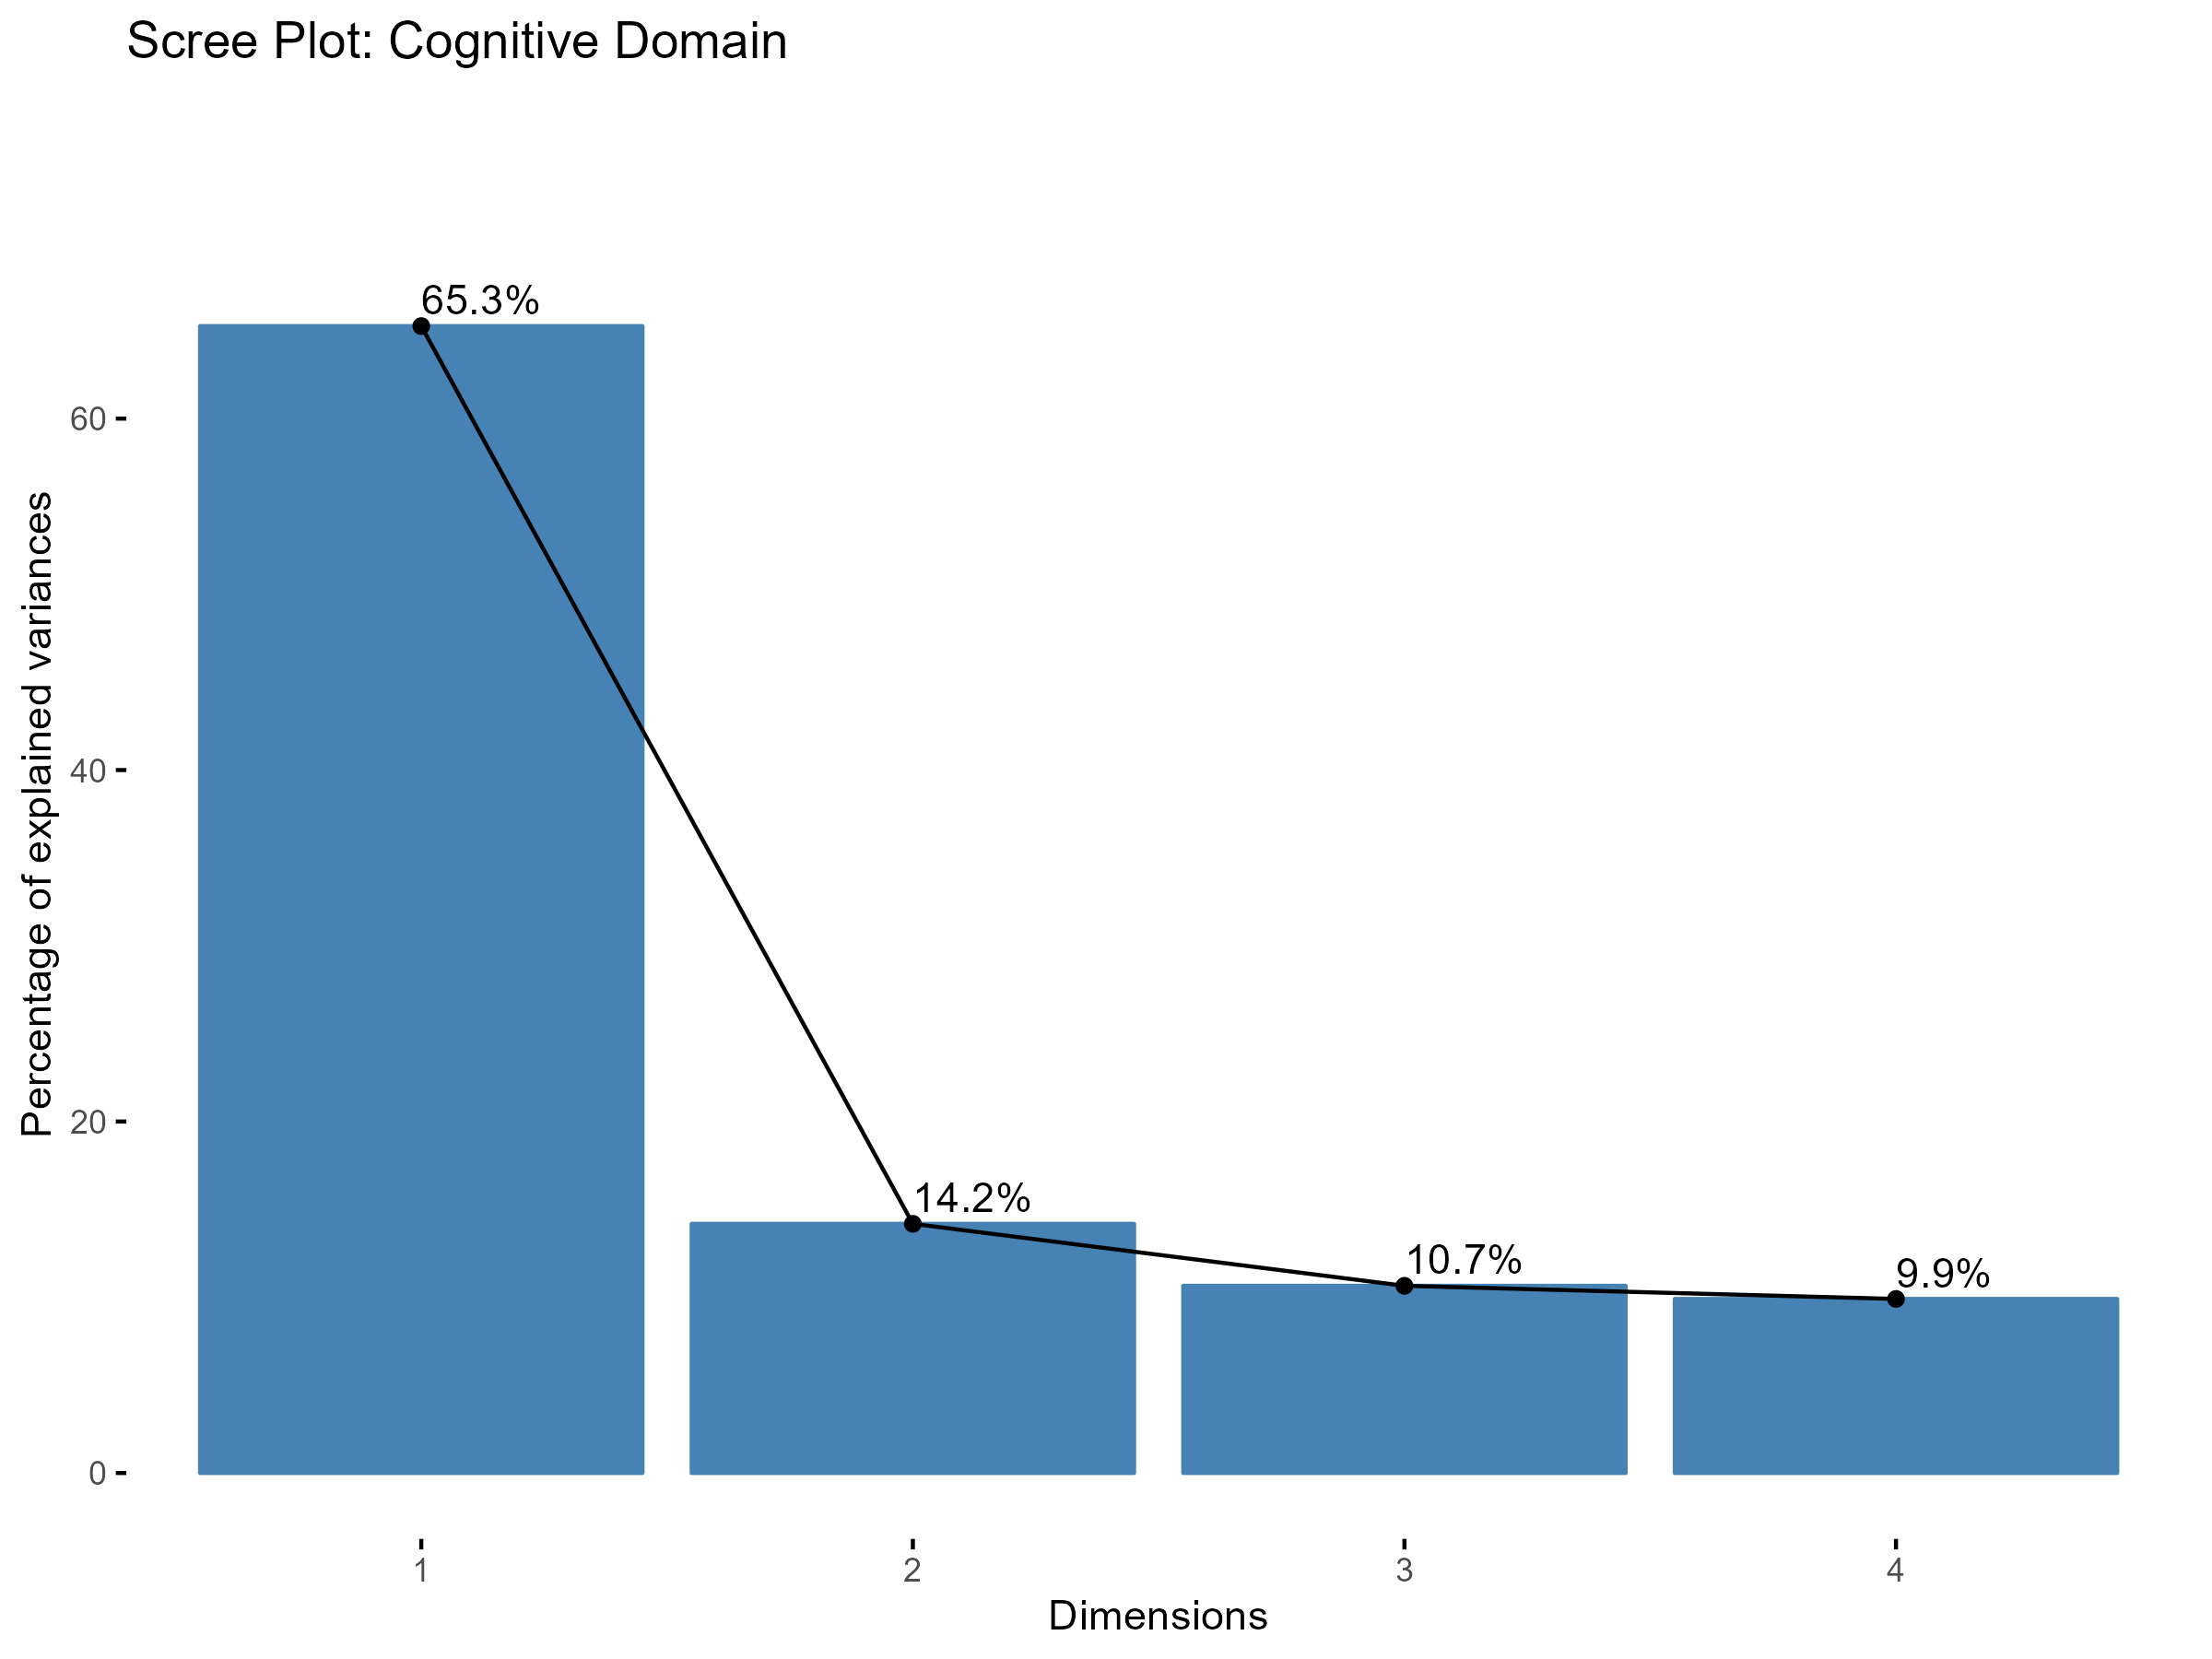
\includegraphics[width=0.7\textwidth,height=\textheight]{imgs/scree_plot_cognitive.png}

}

\caption{Scree plot for the cognitive domain}

\end{figure}

\hypertarget{pca-results--ageing-in-place-domain}{%
\section{PCA results -Ageing in place
domain:}\label{pca-results--ageing-in-place-domain}}

\begin{figure}

{\centering 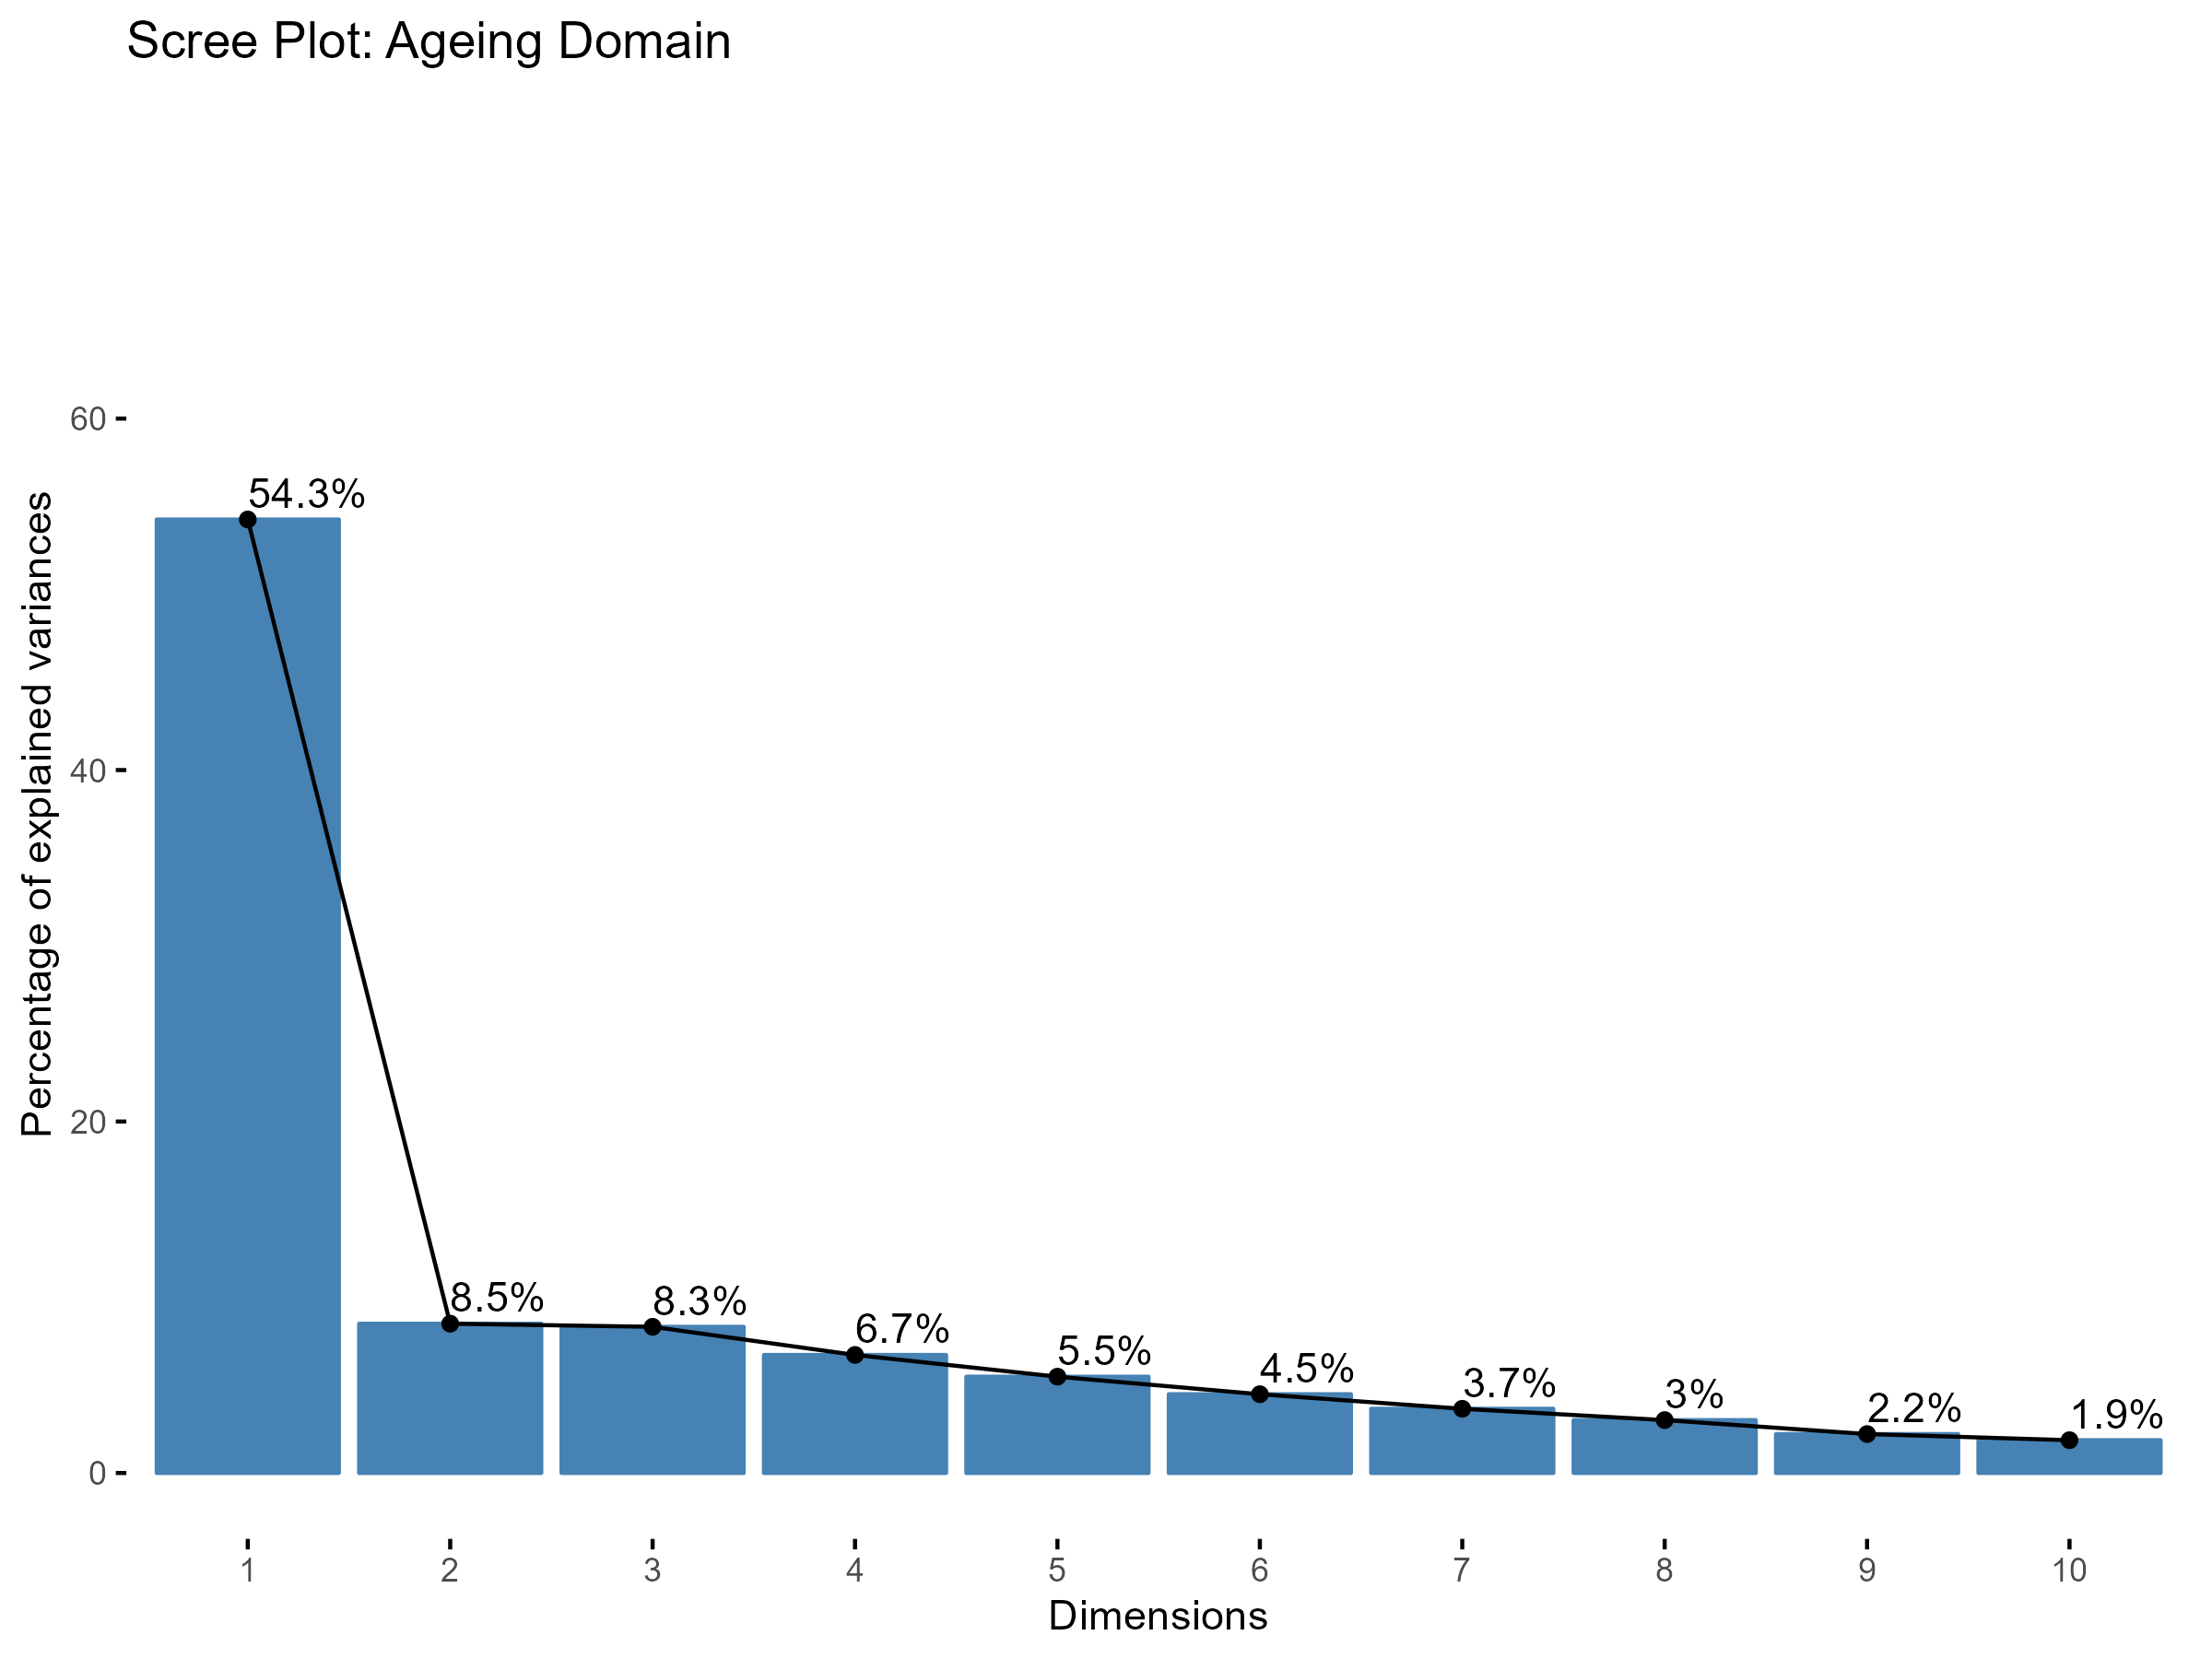
\includegraphics[width=0.7\textwidth,height=\textheight]{imgs/scree_plot_ageing.png}

}

\caption{Scree plot for the ageing domain}

\end{figure}

\hypertarget{pca-results--variables-contribution}{%
\section{PCA results -Variables
contribution:}\label{pca-results--variables-contribution}}

\begin{figure}

{\centering 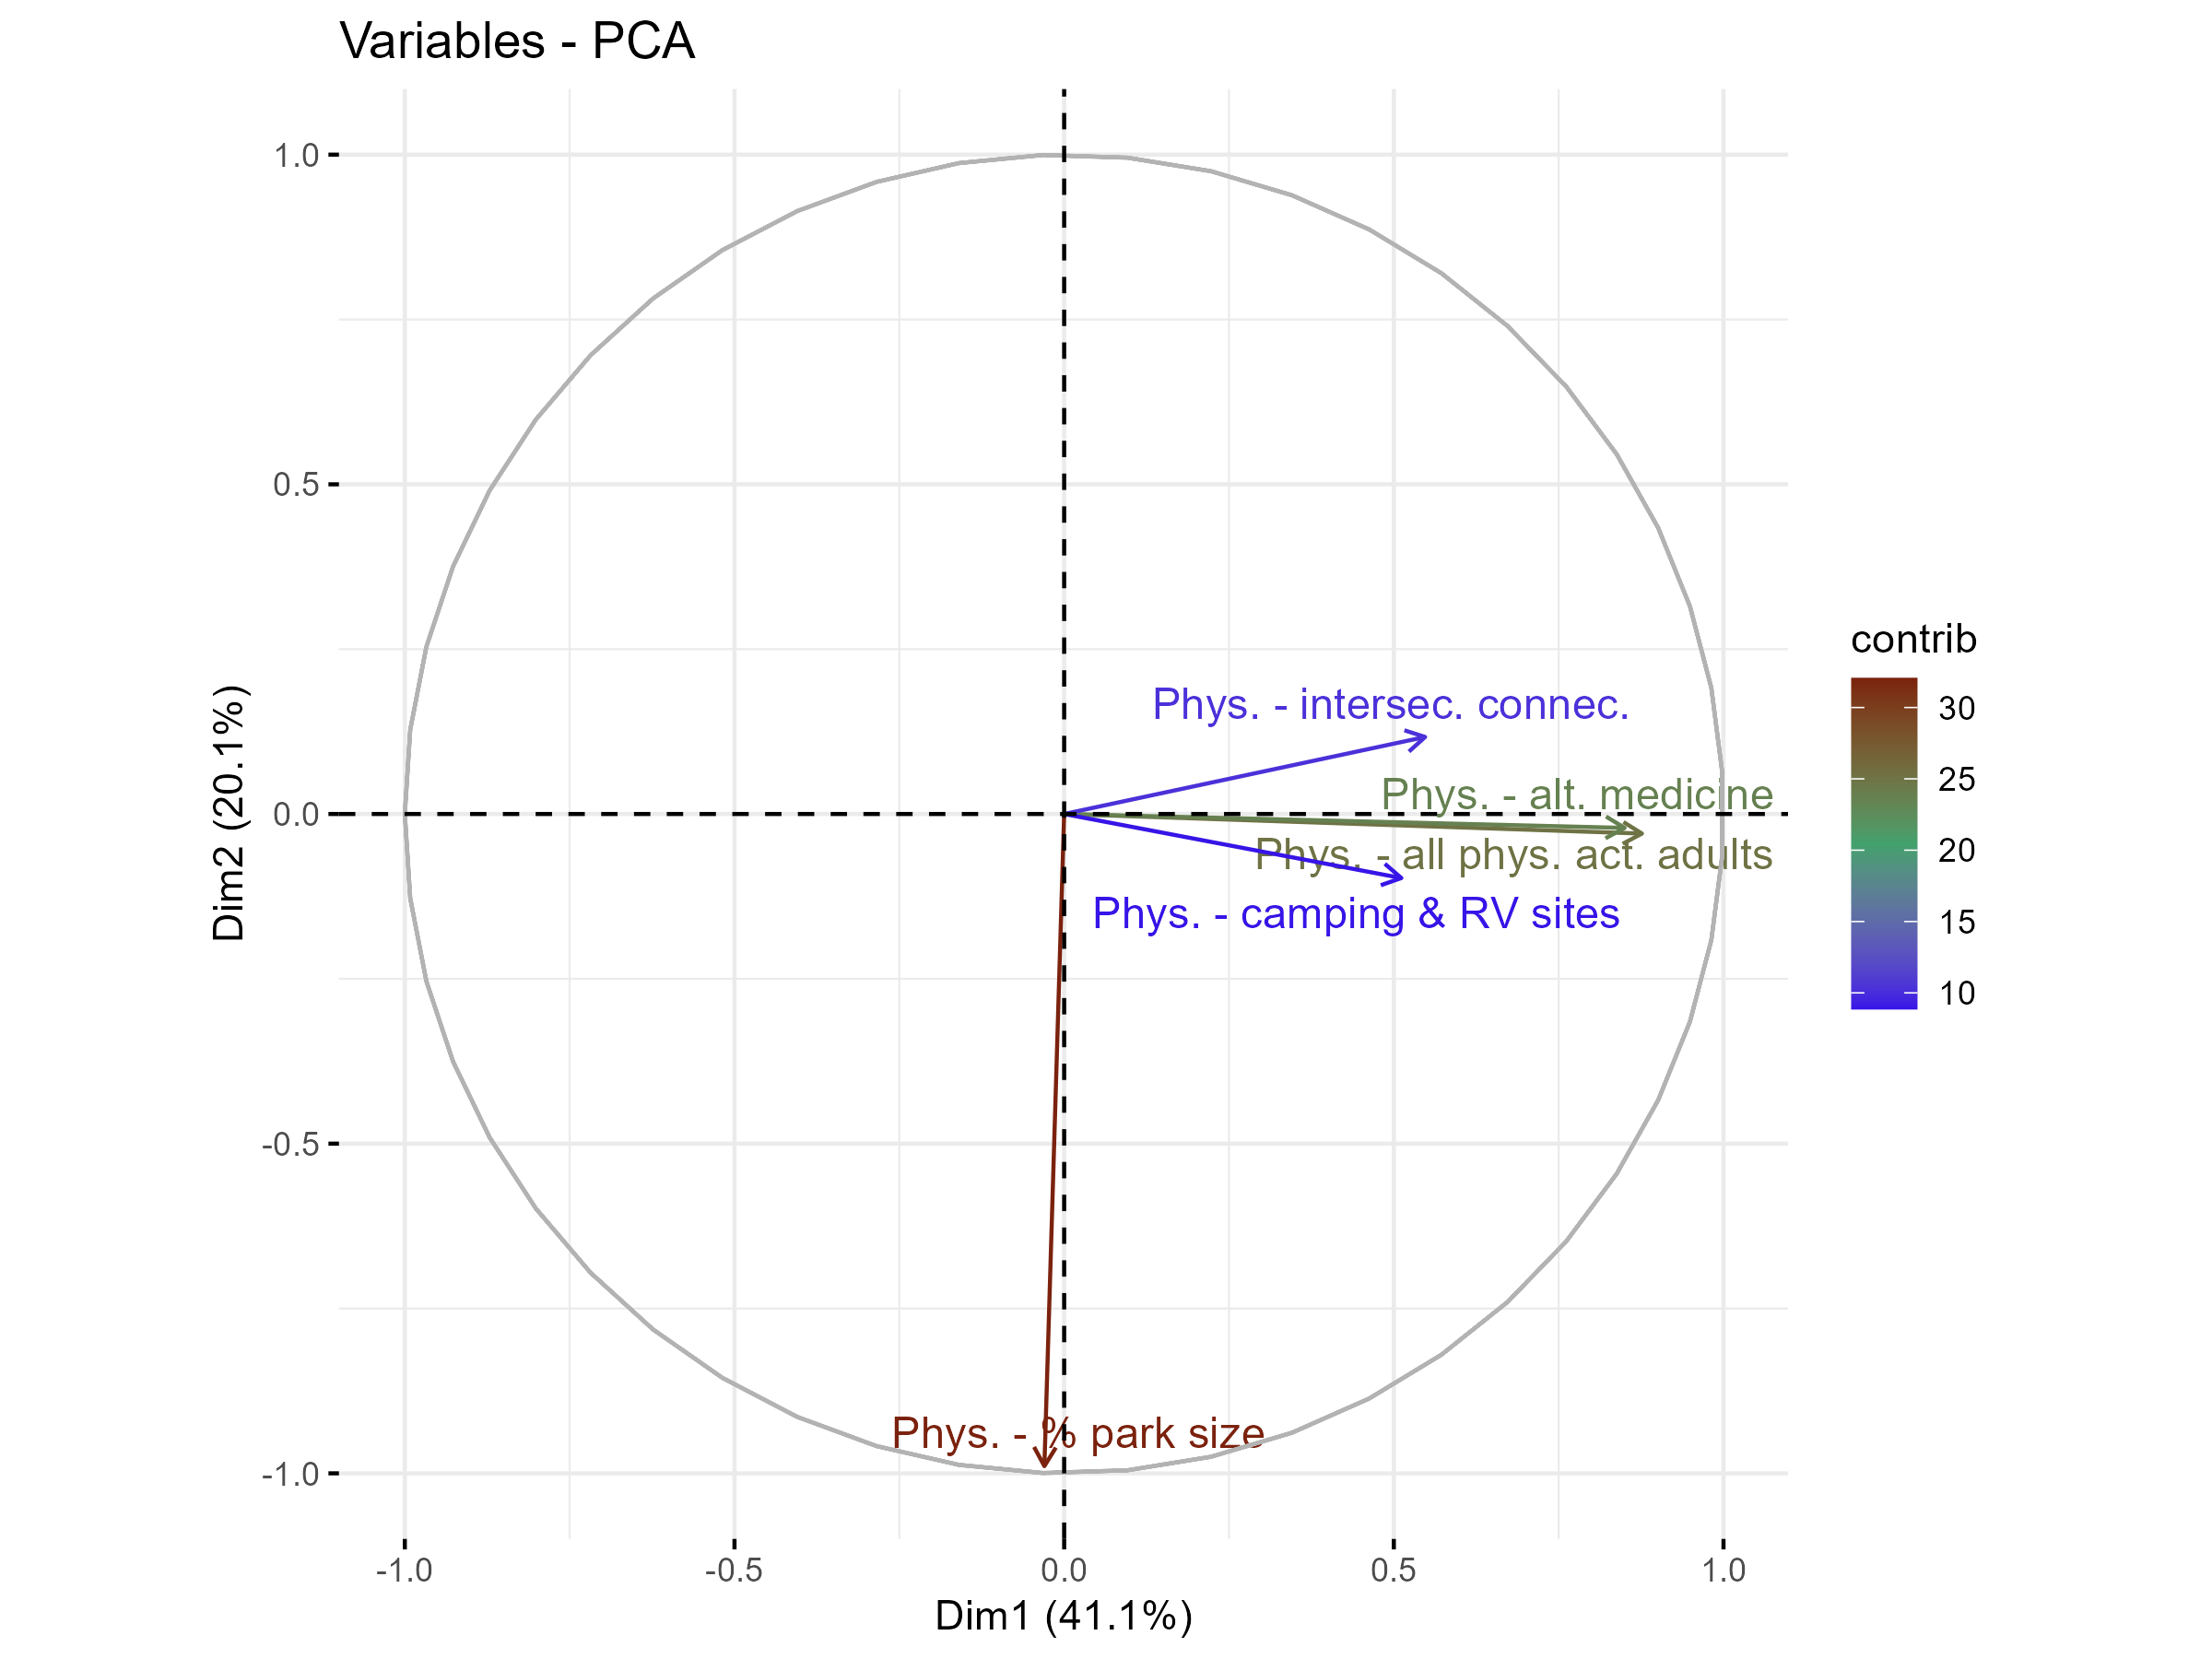
\includegraphics[width=0.7\textwidth,height=\textheight]{imgs/pca_var_physical.png}

}

\caption{most influential variables in the physical domain}

\end{figure}

\hypertarget{pca-results--variables-contribution-1}{%
\section{PCA results -Variables
contribution:}\label{pca-results--variables-contribution-1}}

\begin{figure}

{\centering 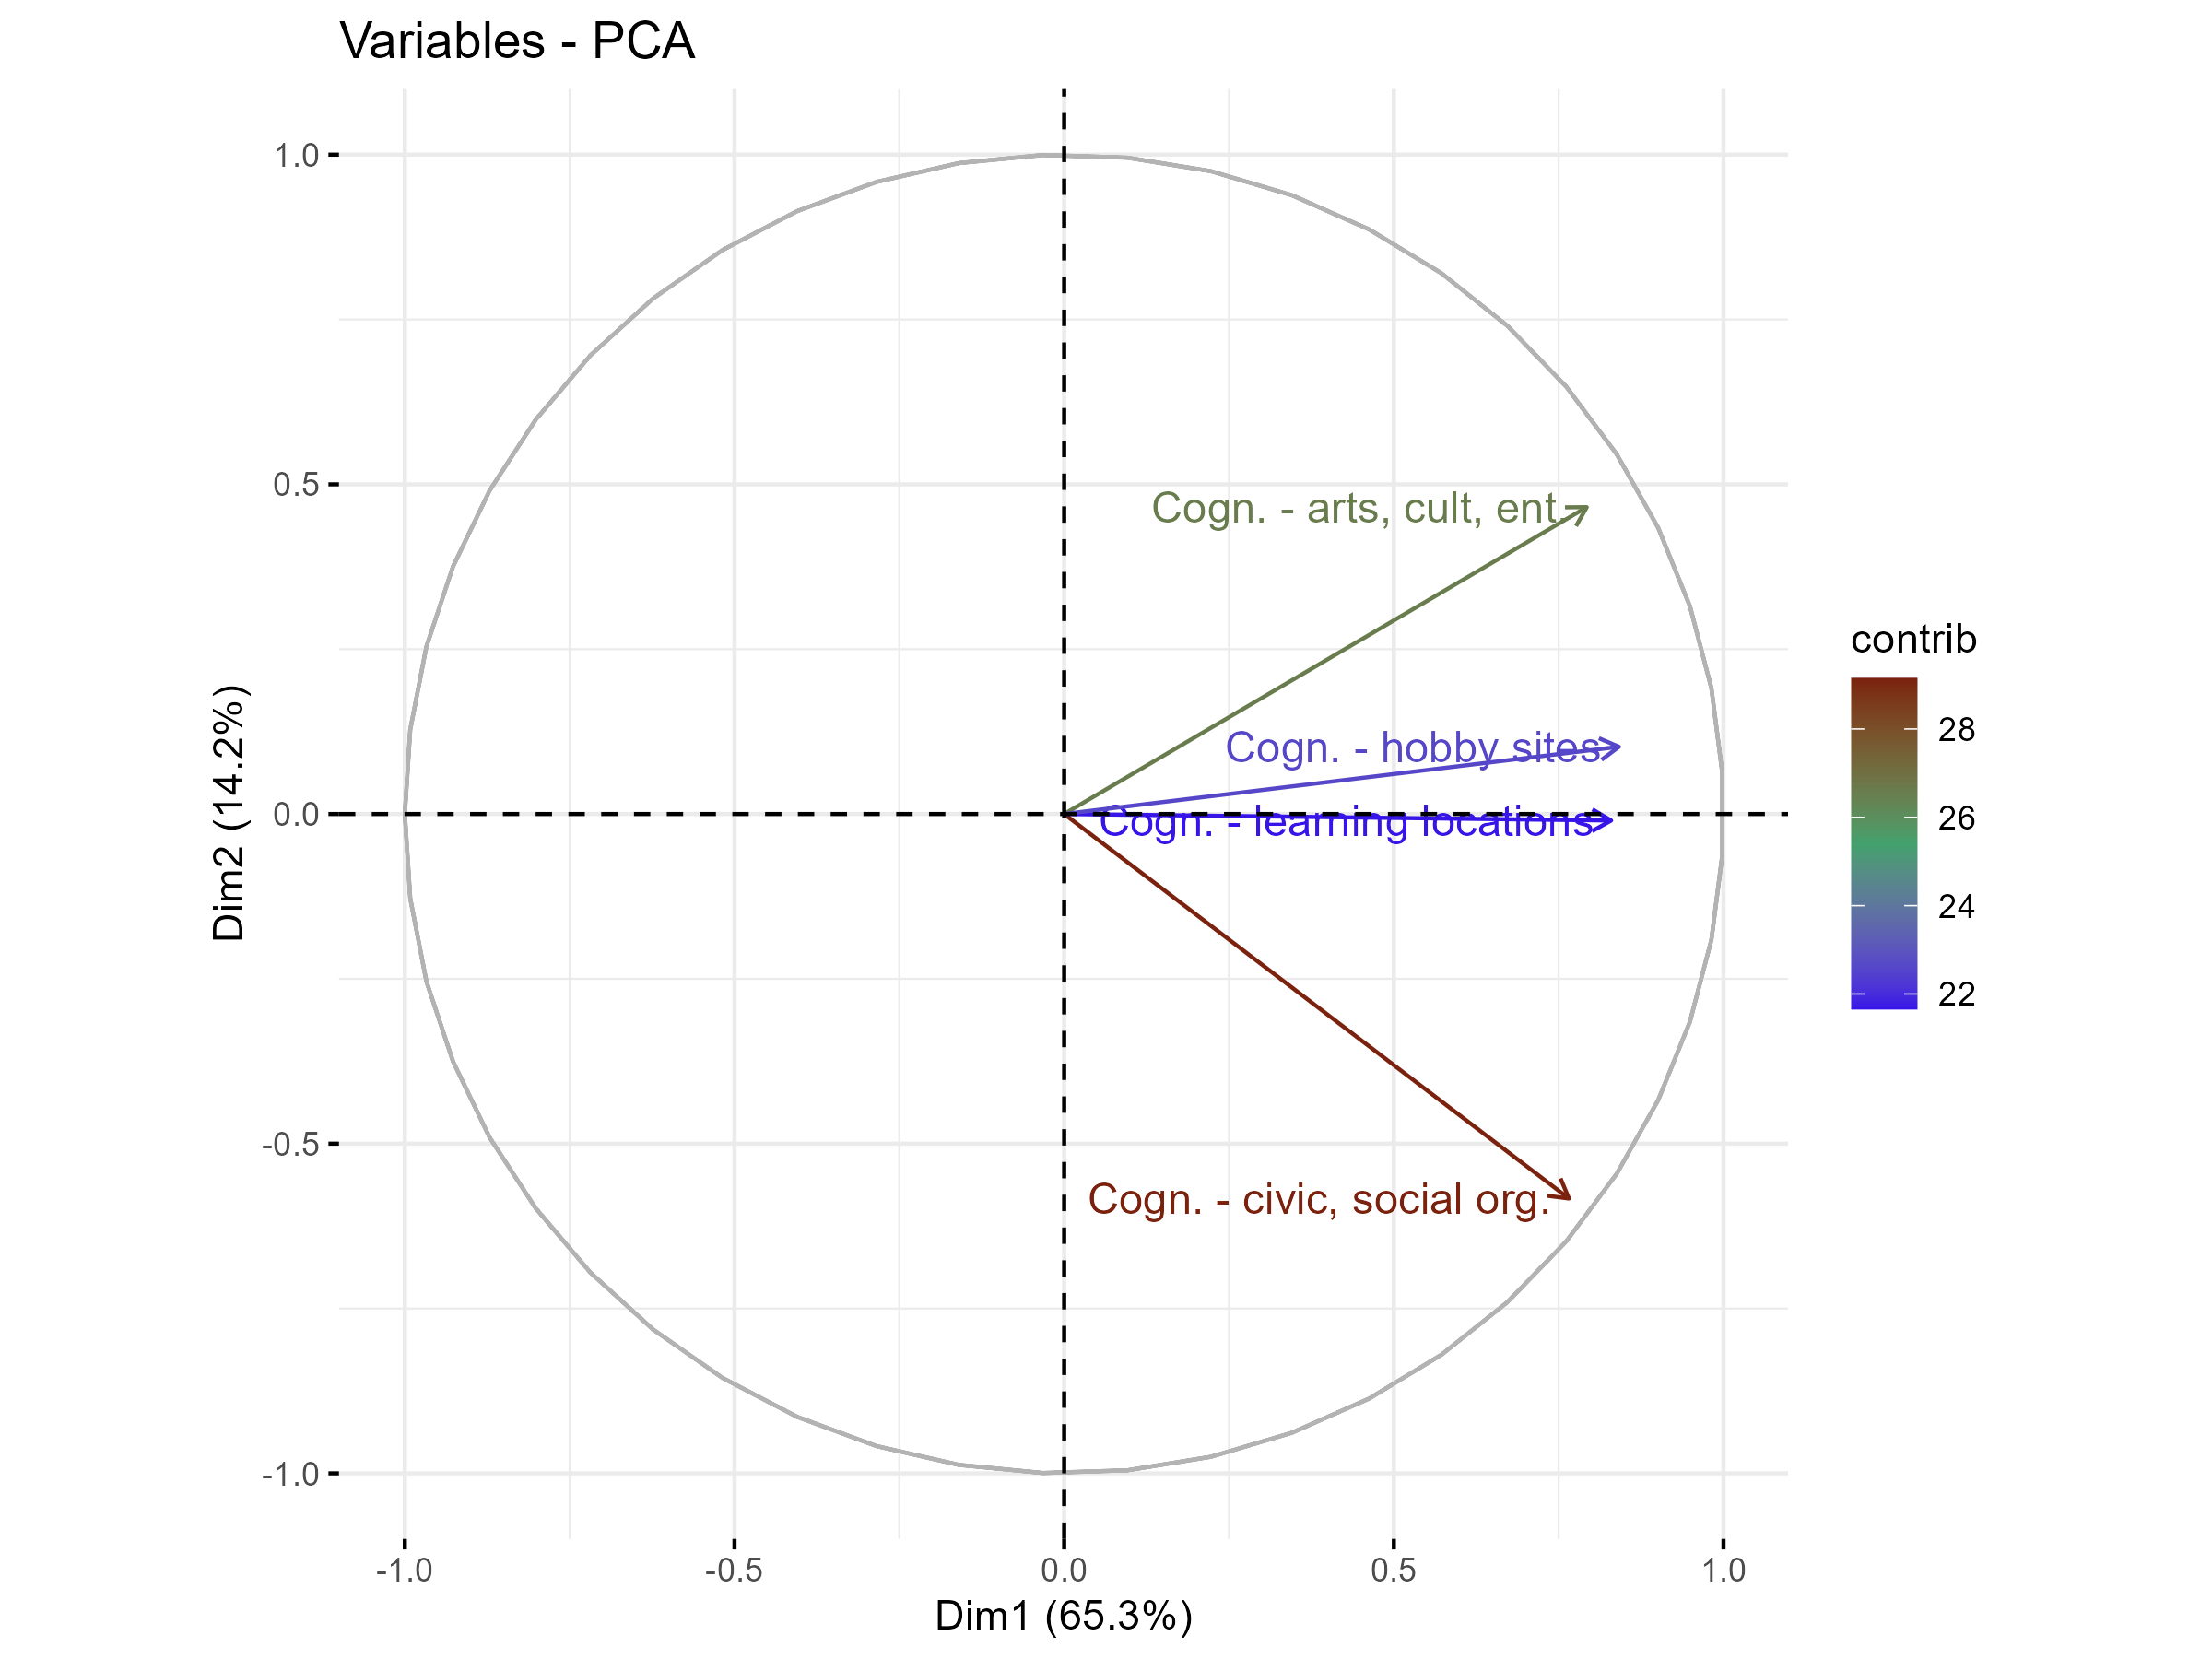
\includegraphics[width=0.7\textwidth,height=\textheight]{imgs/pca_var_cognitive.png}

}

\caption{most influential variables in the ageing domain}

\end{figure}

\hypertarget{pca-results--variables-contribution-2}{%
\section{PCA results -Variables
contribution:}\label{pca-results--variables-contribution-2}}

\begin{figure}

{\centering 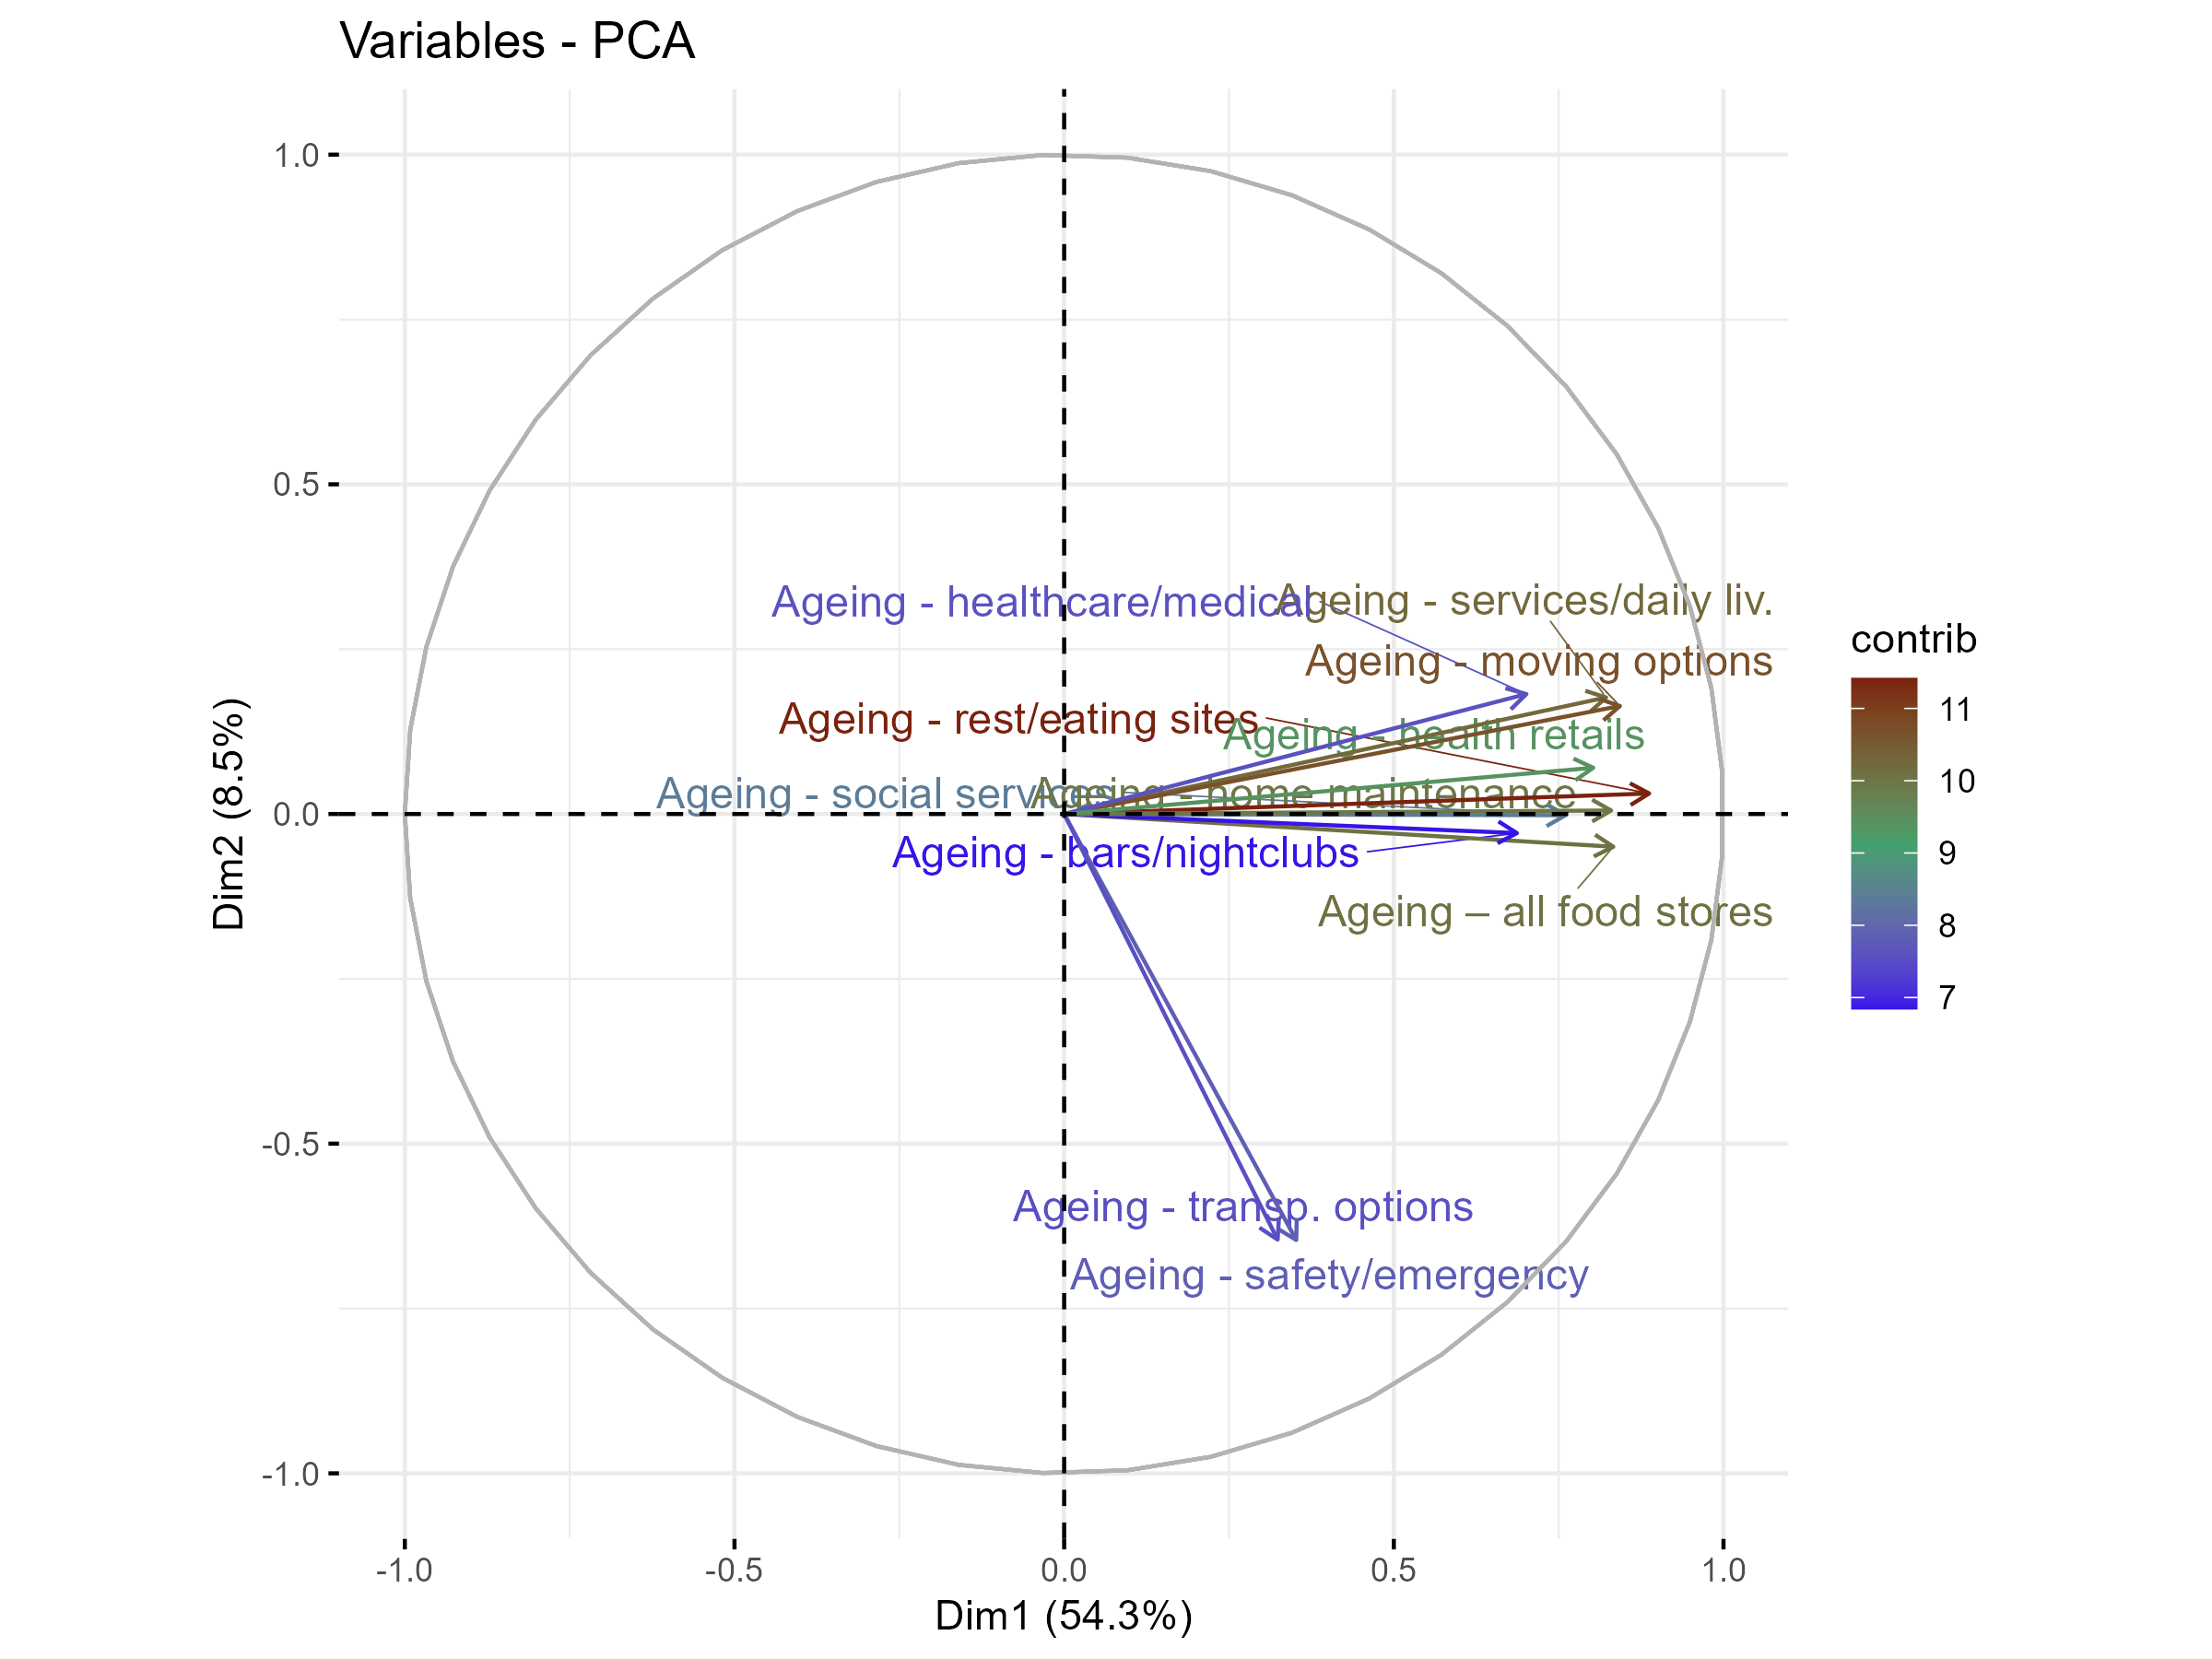
\includegraphics[width=0.7\textwidth,height=\textheight]{imgs/pca_var_ageing.png}

}

\caption{most influential variables in the physical domain}

\end{figure}

\hypertarget{pca-results--correlations-among-pcas}{%
\section{PCA results -Correlations among
PCAs:}\label{pca-results--correlations-among-pcas}}

\begin{figure}

{\centering 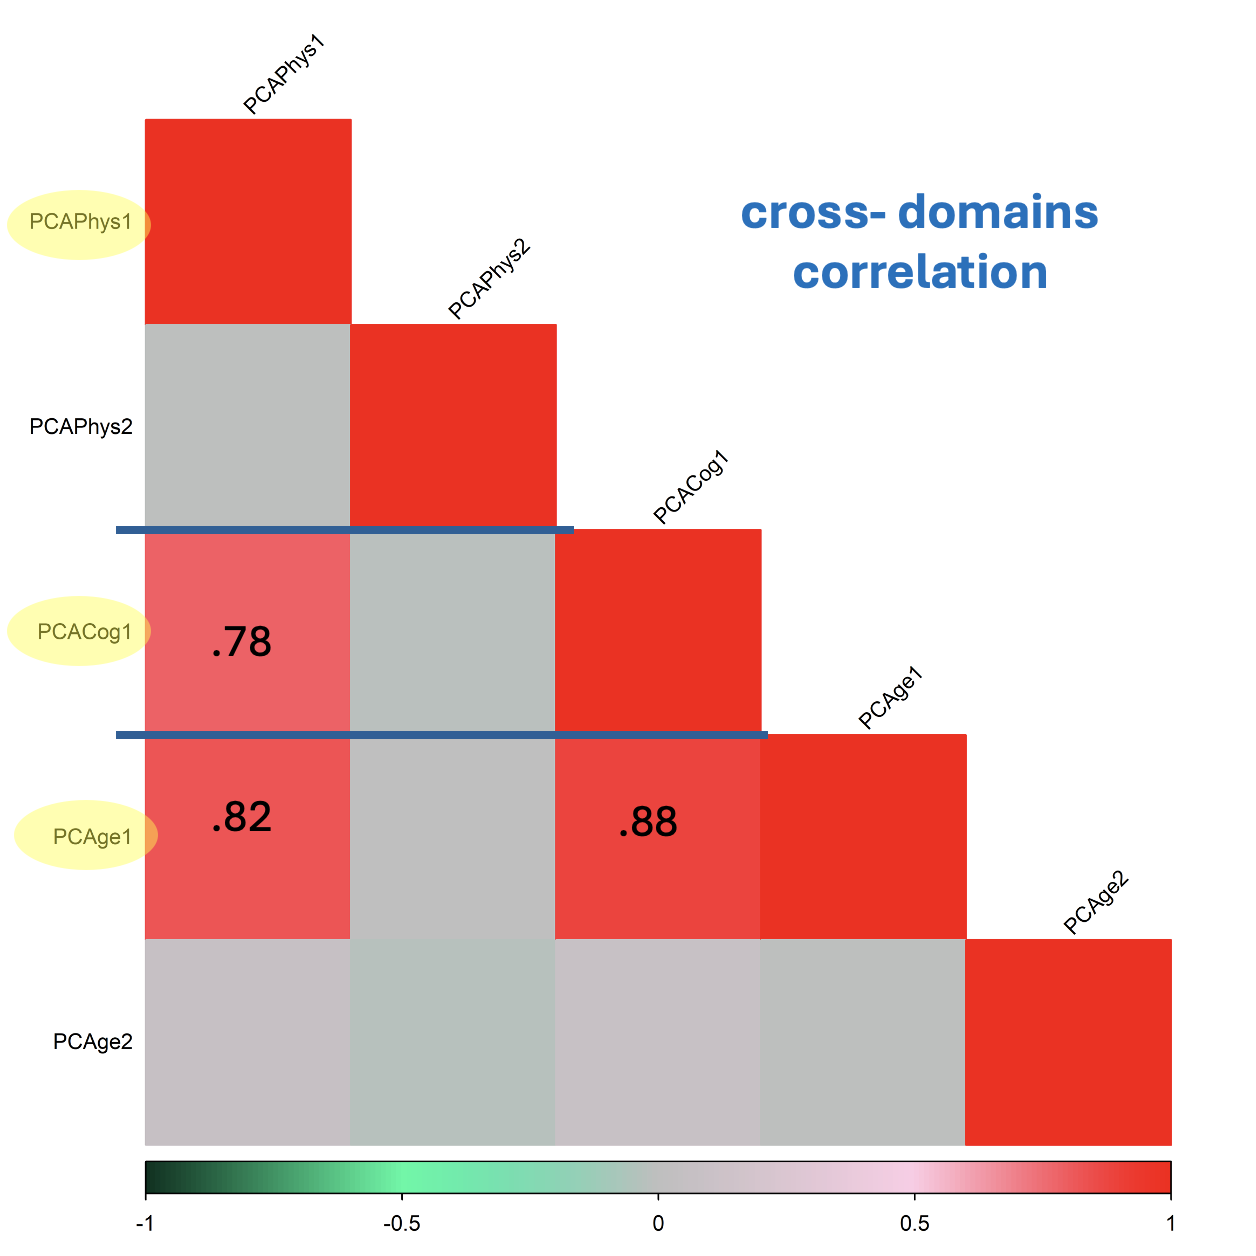
\includegraphics[width=0.5\textwidth,height=\textheight]{imgs/crossDomainCorrelations.png}

}

\caption{correlation among PCAs - which ones to choose?}

\end{figure}

\hypertarget{mapping-pcas}{%
\section{Mapping PCAs}\label{mapping-pcas}}

\begin{figure}

{\centering 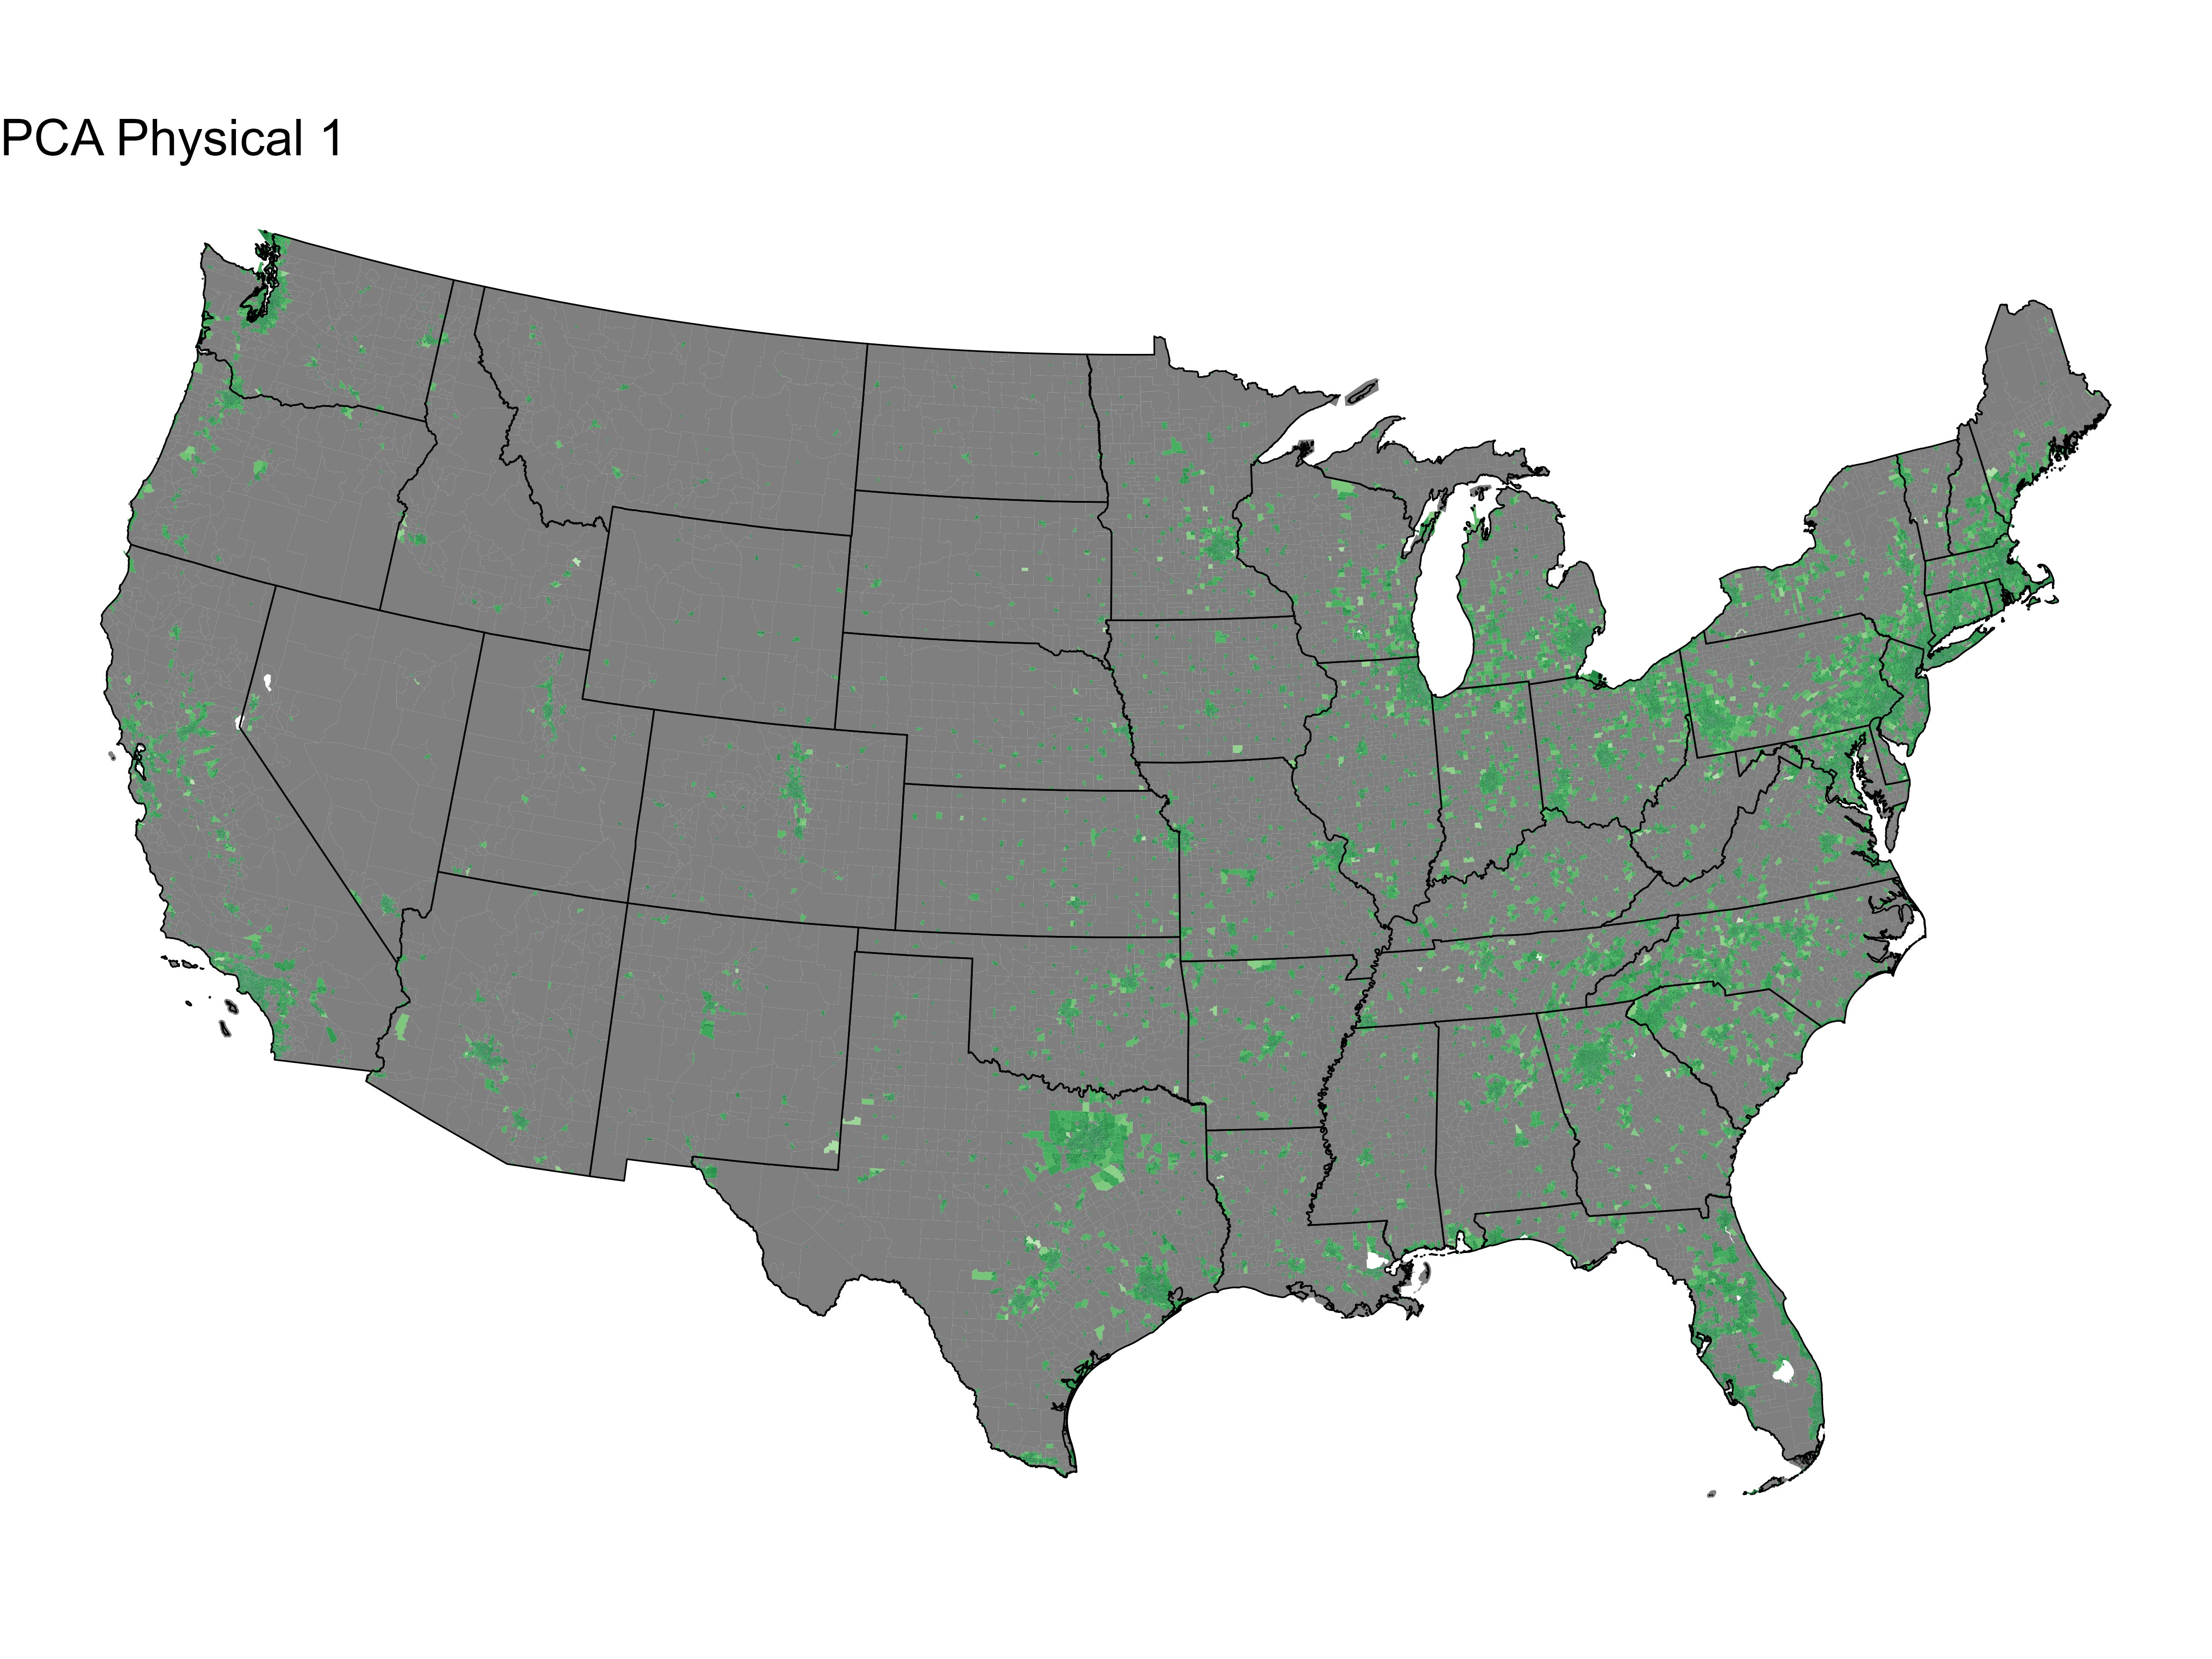
\includegraphics[width=0.7\textwidth,height=\textheight]{imgs/PCAPhys1.png}

}

\caption{first PCA in physical domain}

\end{figure}

\hypertarget{mapping-pcas-1}{%
\section{Mapping PCAs}\label{mapping-pcas-1}}

\begin{figure}

{\centering 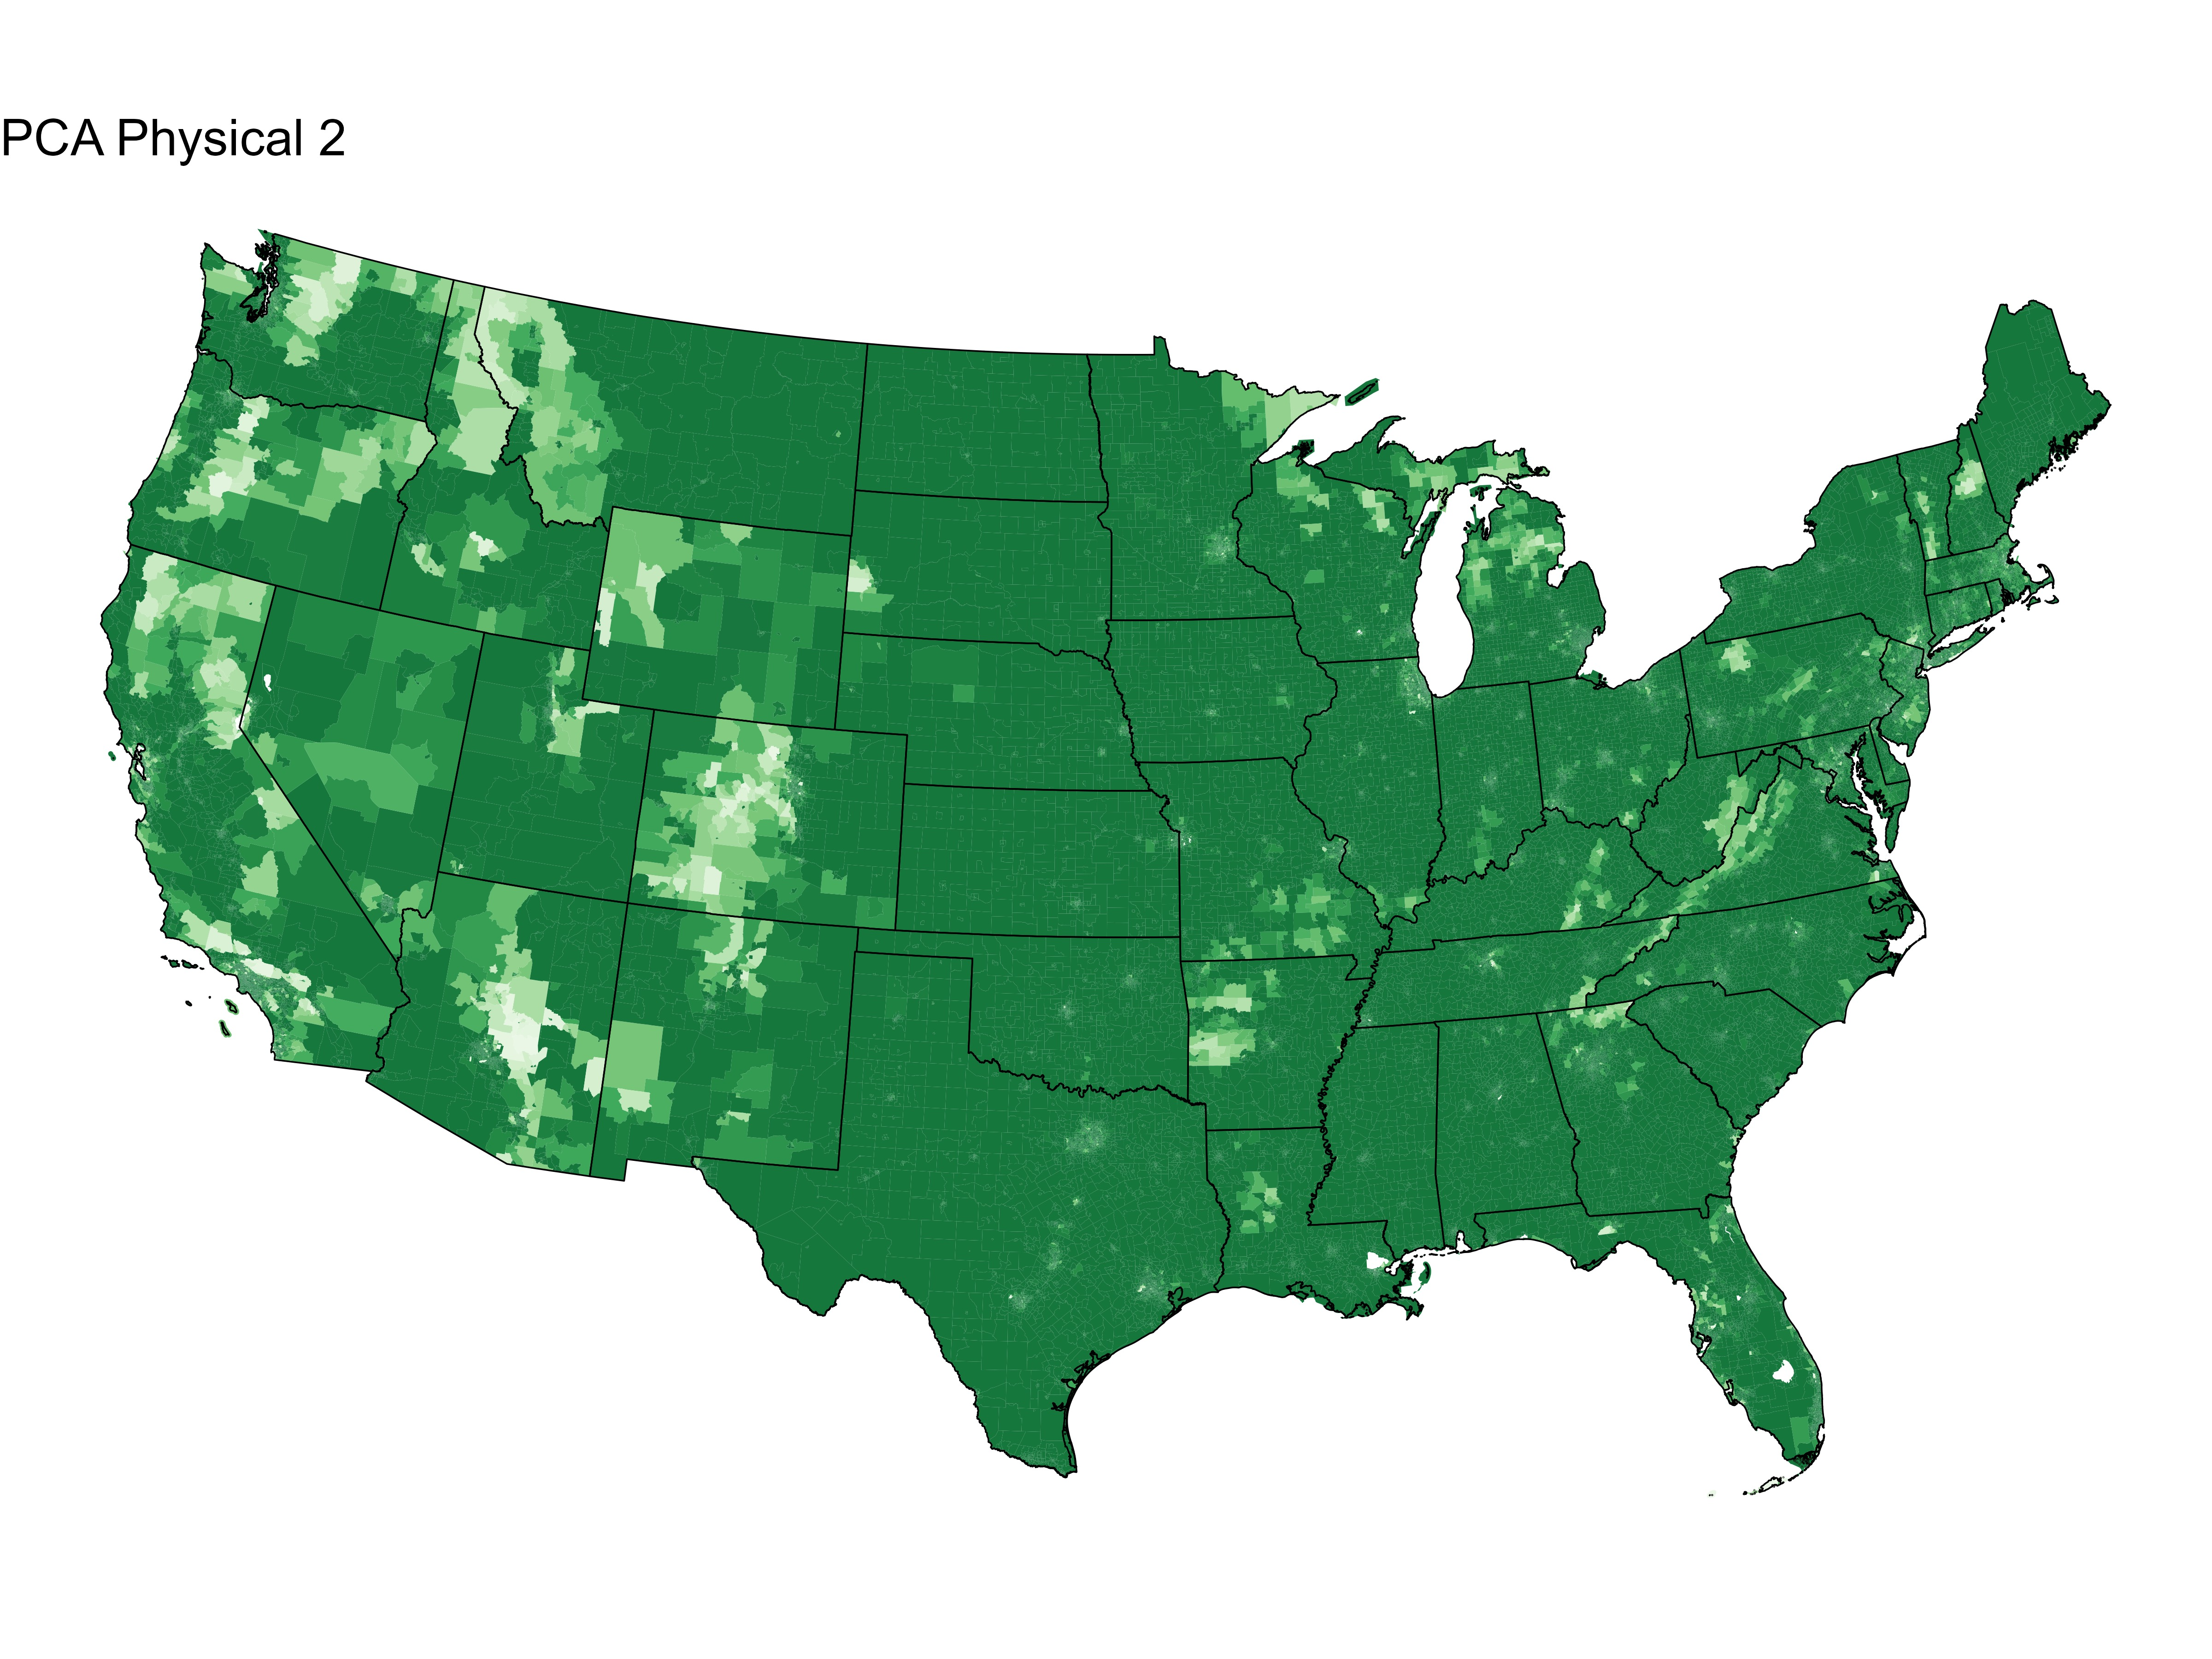
\includegraphics[width=0.7\textwidth,height=\textheight]{imgs/PCAPhys2.png}

}

\caption{Second PCA in physical domain}

\end{figure}

\hypertarget{mapping-pcas-2}{%
\section{Mapping PCAs}\label{mapping-pcas-2}}

\begin{figure}

{\centering \includegraphics[width=0.7\textwidth,height=\textheight]{imgs/PCAAge2.png}

}

\caption{Second PCA in ageing in place domain}

\end{figure}

\hypertarget{methods-kmeans-algorithm}{%
\section{\texorpdfstring{Methods: \texttt{kmeans}
algorithm}{Methods: kmeans algorithm}}\label{methods-kmeans-algorithm}}

\begin{itemize}
\tightlist
\item
  \textbf{Observations} for each geographic unit \(i\) in matrix
  \(\mathbf {x}\)

  \begin{itemize}
  \tightlist
  \item
    changes over time, \ldots{} different variables
  \item
    rescale your data (e.g.~between 0 and 1)
  \end{itemize}
\item
  Find \(k\) clusters \(S = \{S_{1}, S_{2}, ..., S_{k}\}\) so that sum
  of square within the cluster is minimized
  \(\displaystyle \mathop {\operatorname {arg\,min} } _{\mathbf {S} }\sum _{i=1}^{k}\sum _{\mathbf {x} \in S_{i}}\left\|\mathbf {x} -{\boldsymbol {\mu }}_{i}\right\|^{2}\)
  with\\
  \(\boldsymbol {\mu _{i}}={\frac {1}{|S_{i}|}}\sum_{\mathbf {x} \in S_{i}}\mathbf {x}\)
\item
  Number of clusters \(k\)? Calinski-Harabasz stopping rule
\end{itemize}

\hypertarget{k-means-result-1}{%
\section{k-means result (1):}\label{k-means-result-1}}

\begin{figure}

{\centering 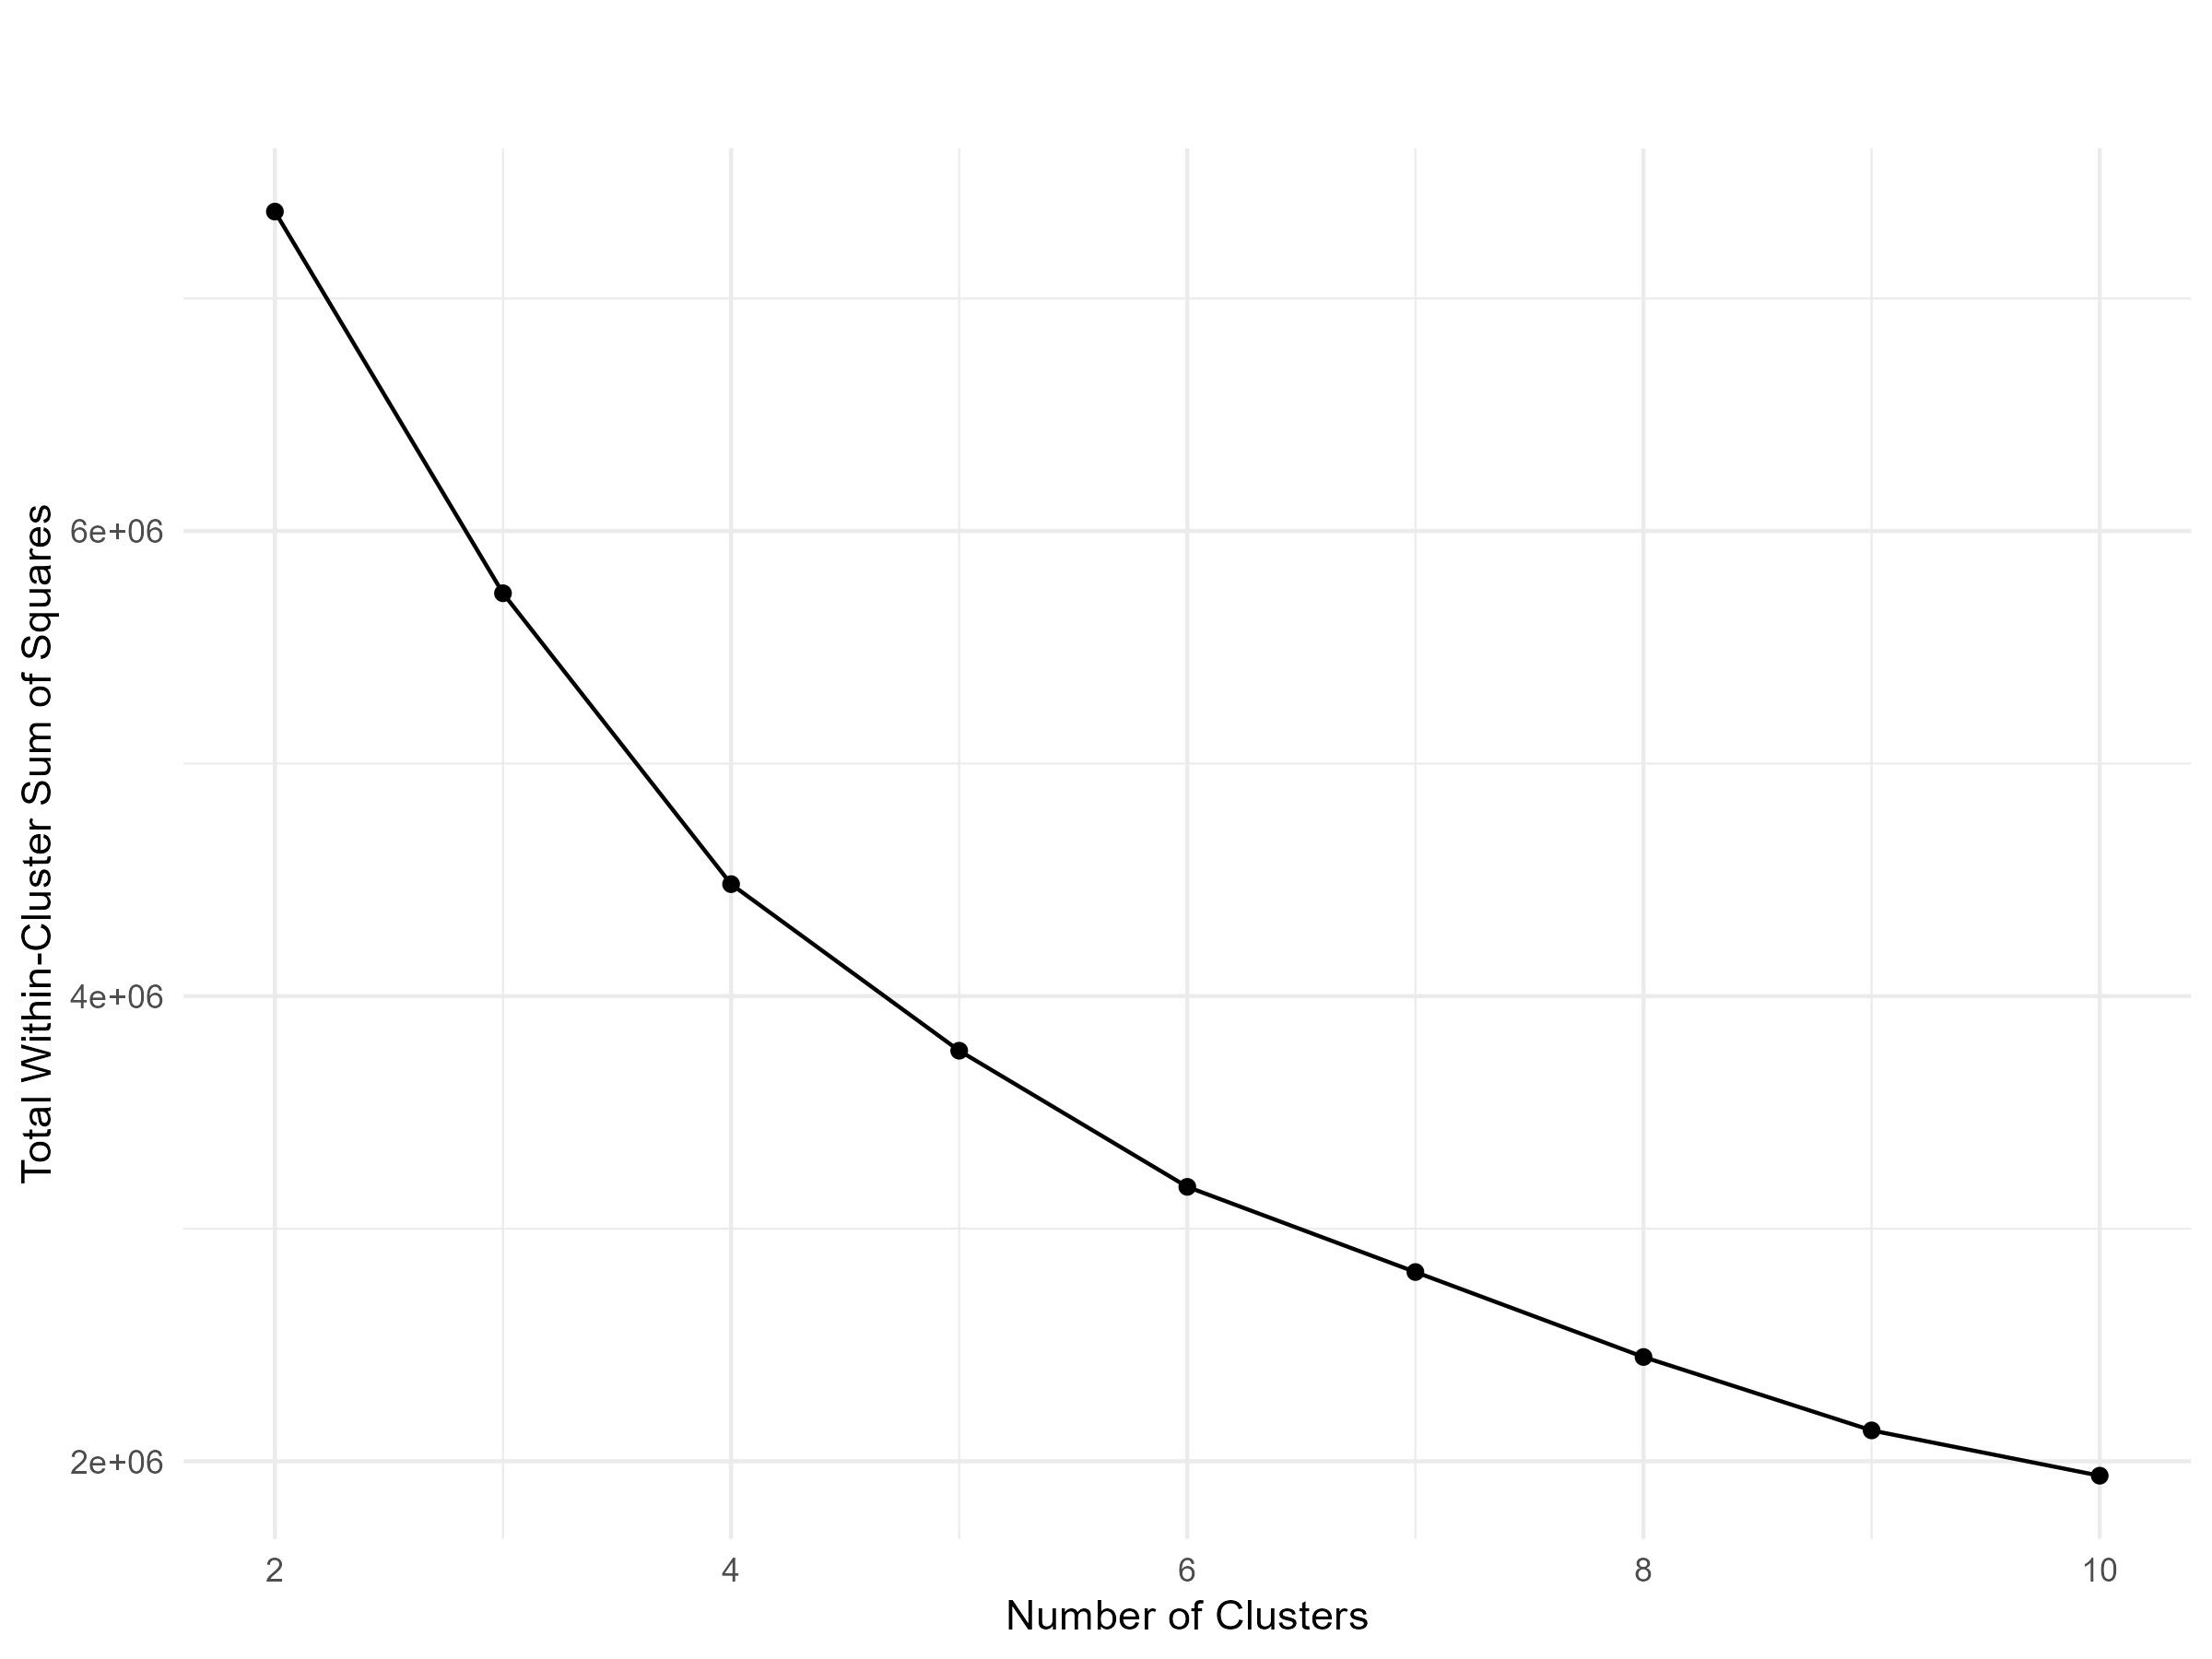
\includegraphics[width=0.7\textwidth,height=\textheight]{imgs/elbow_plot.png}

}

\caption{decreasing within clusters sum of squares}

\end{figure}

\hypertarget{k-means-results-2}{%
\section{k-means results (2):}\label{k-means-results-2}}

\begin{figure}

{\centering 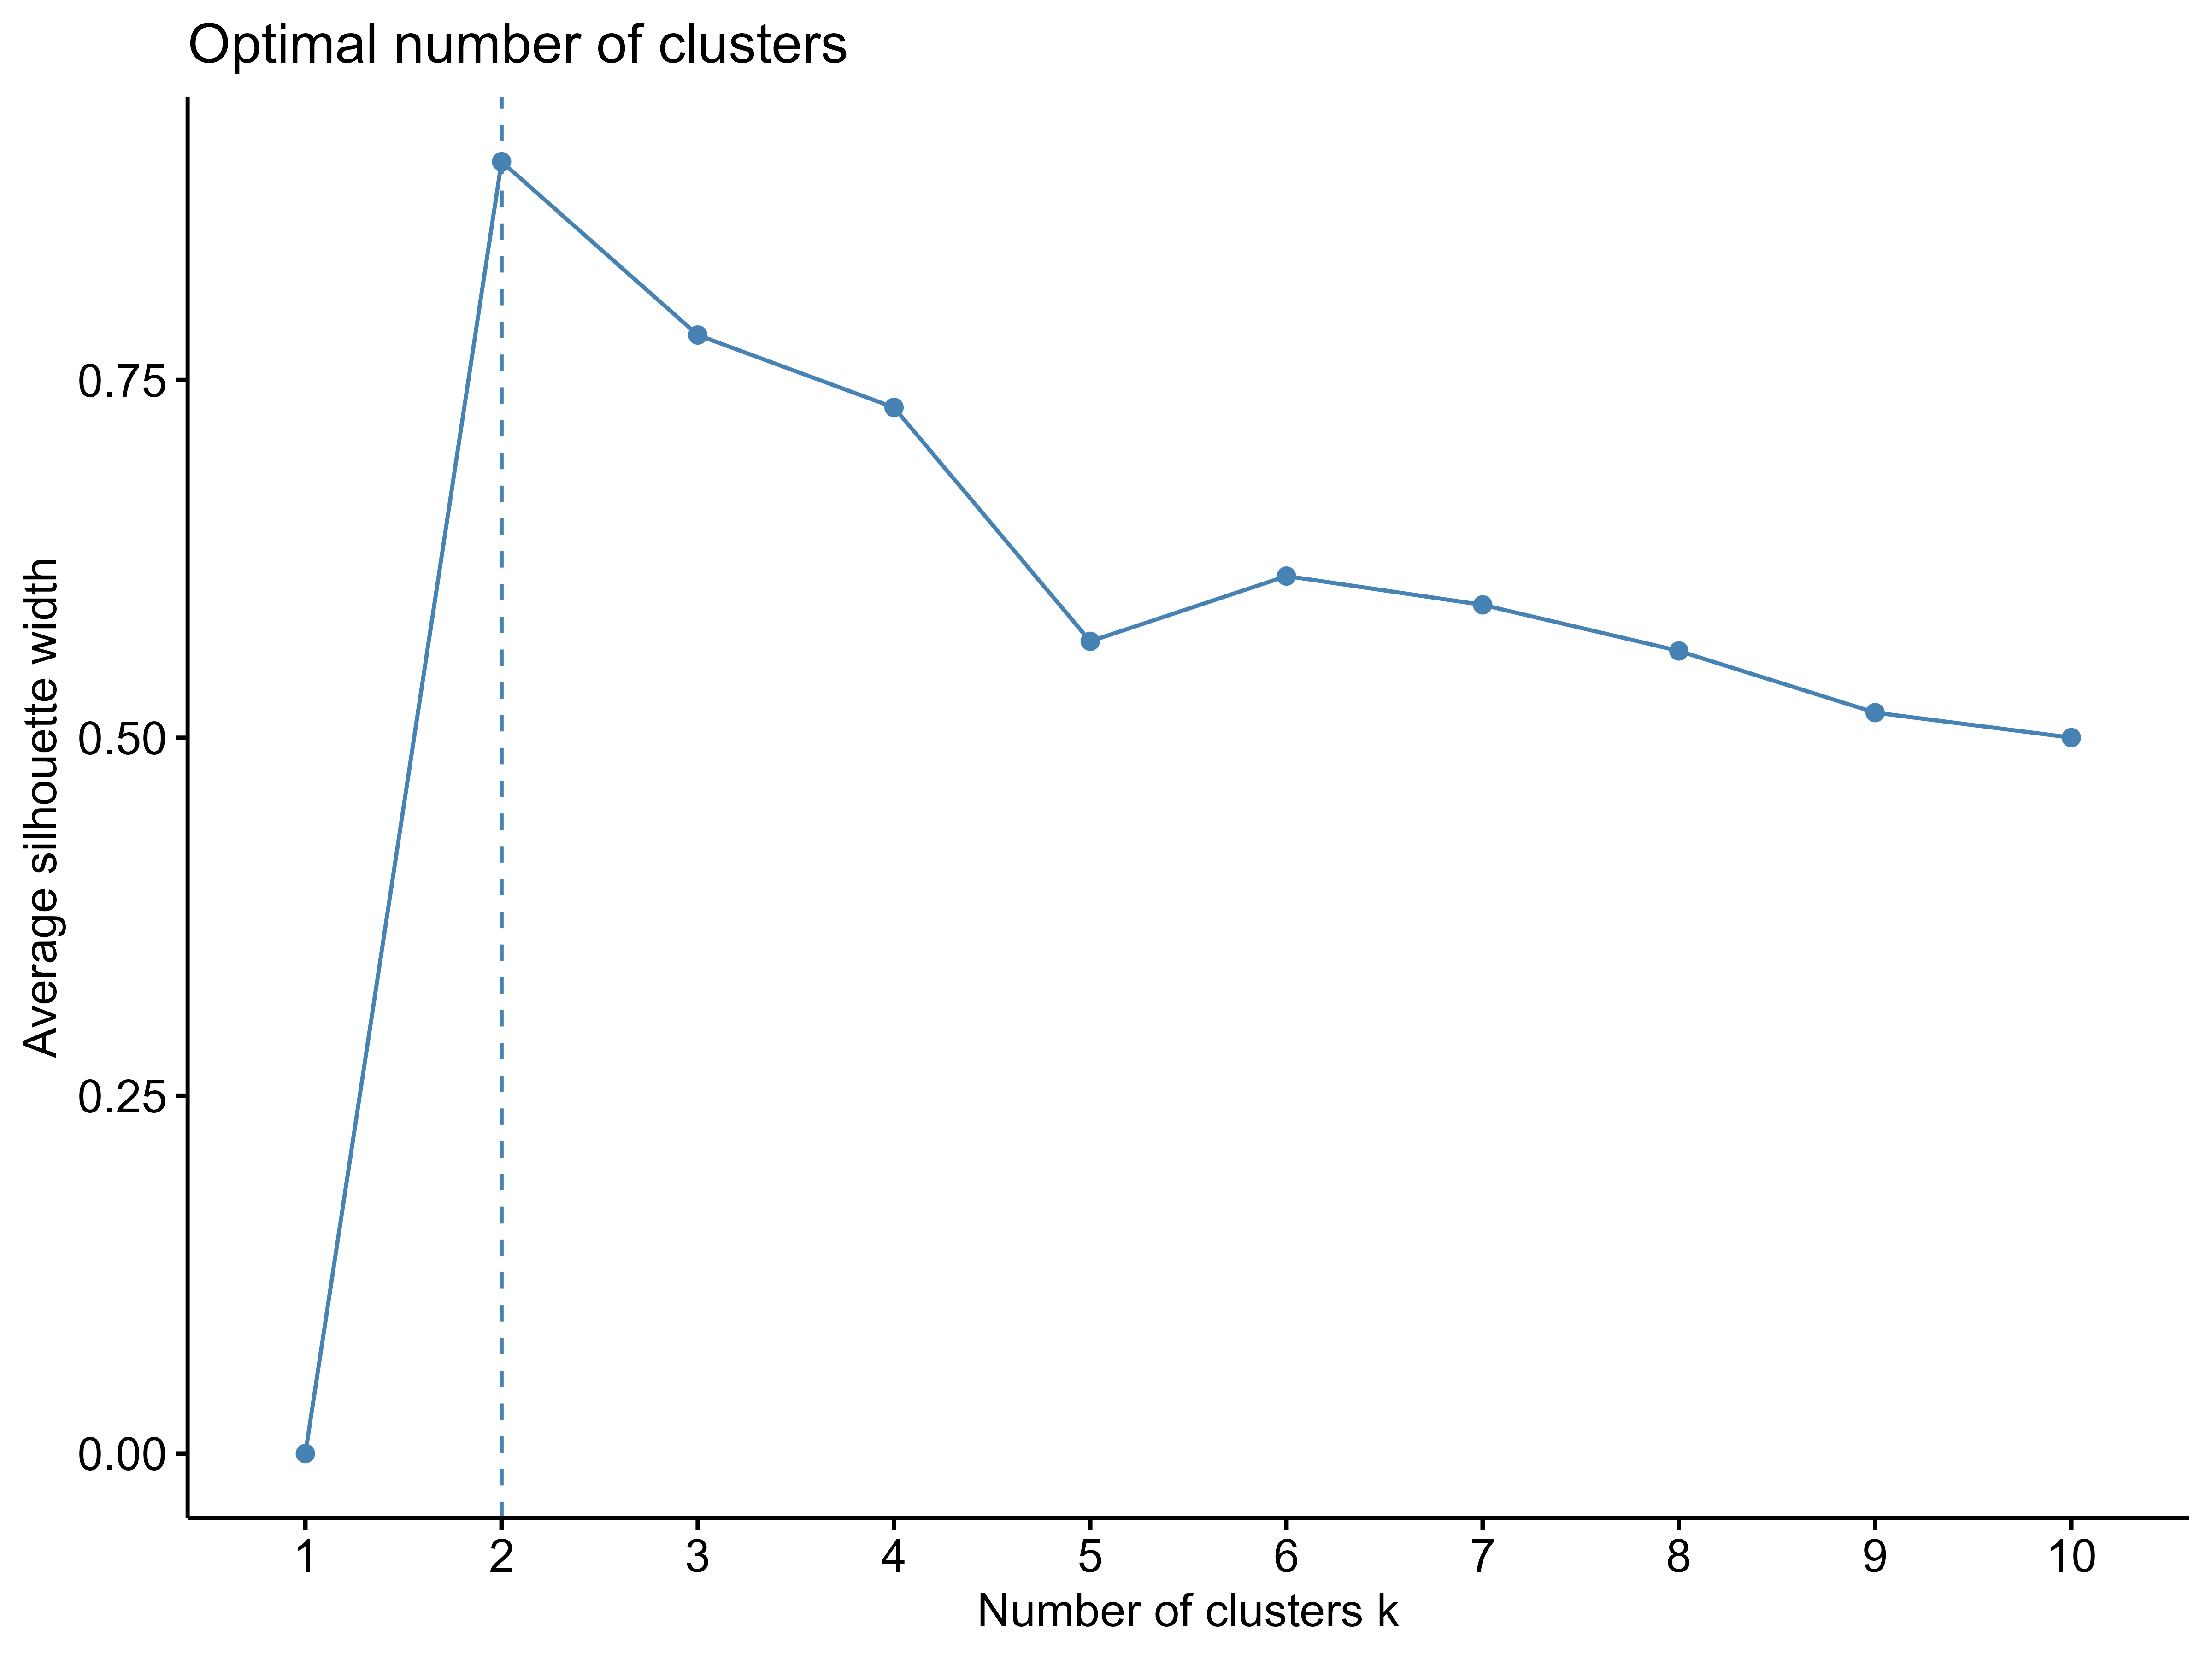
\includegraphics[width=0.7\textwidth,height=\textheight]{imgs/silhouette_plot.png}

}

\caption{silhouette plot (2 or 6 clusters?)}

\end{figure}

\hypertarget{k-means-results-3}{%
\section{k-means results (3):}\label{k-means-results-3}}

\begin{figure}

{\centering 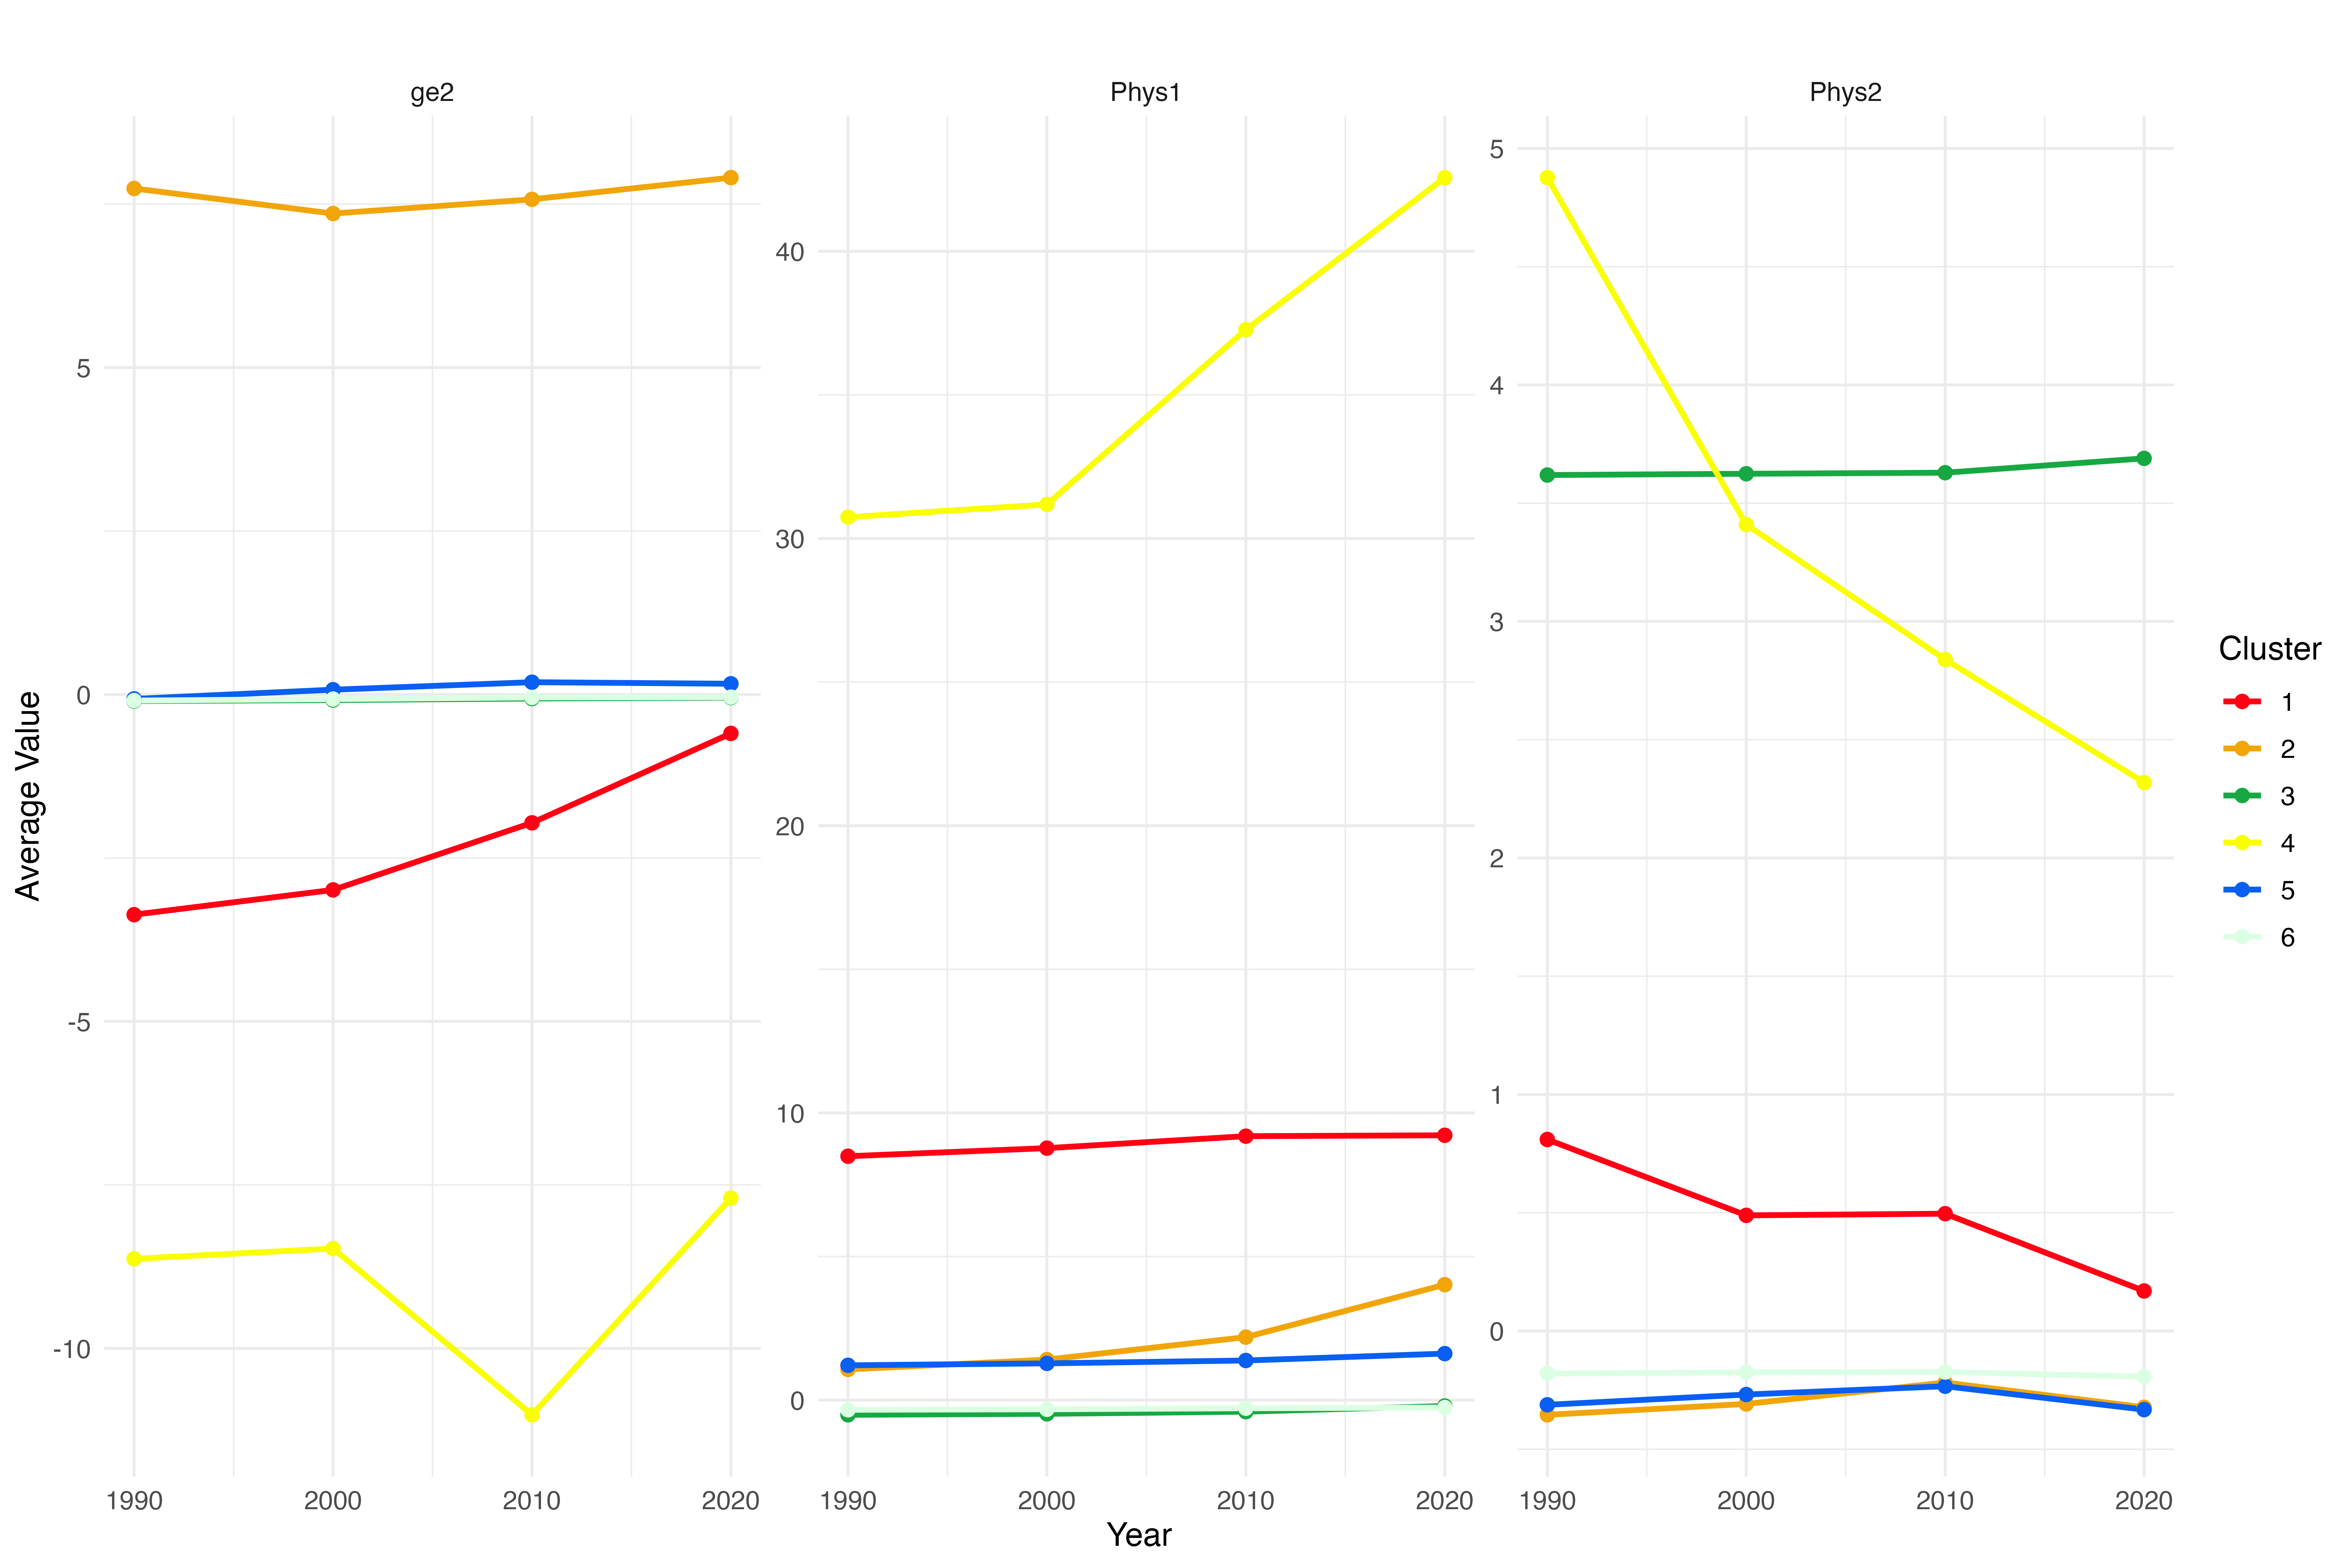
\includegraphics[width=0.7\textwidth,height=\textheight]{imgs/ClusterCharacteristicsB.png}

}

\caption{What characterizes these 6 clusters?}

\end{figure}

\hypertarget{cluster-characteristics-1}{%
\section{Cluster characteristics (1)}\label{cluster-characteristics-1}}

\begin{itemize}
\tightlist
\item
  \texttt{cluster\ 1}: Intensely Active Urban Cores (red)

  \begin{itemize}
  \tightlist
  \item
    (n=95 1990 to n=1300 in 2020)
  \item
    Areas with intense physical engagement
  \end{itemize}
\item
  \texttt{cluster\ 2}: Emerging growth centers (orange)

  \begin{itemize}
  \tightlist
  \item
    (n=117 1990 to n=637 in 2020)
  \item
    Emerging as activity hubs (suburban areas)
  \end{itemize}
\end{itemize}

\hypertarget{cluster-characteristics-2}{%
\section{Cluster characteristics (2)}\label{cluster-characteristics-2}}

\begin{itemize}
\tightlist
\item
  \texttt{cluster\ 3}: Green Living (green)

  \begin{itemize}
  \tightlist
  \item
    Areas with a focus on sustainability or outdoor activity
  \item
    Supports green spaces or recreational activities
  \item
    May include towns prioritizing eco-friendly living
  \end{itemize}
\item
  \texttt{cluster\ 4}: High-Intensity Niche Zones (yellow)

  \begin{itemize}
  \tightlist
  \item
    Very high activity levels of physical engagement
  \item
    High-performance sports are prevalent
  \item
    (e.g.~lower Manhattan, center City in Philly)
  \end{itemize}
\end{itemize}

\hypertarget{cluster-characteristics-3}{%
\section{Cluster characteristics (3)}\label{cluster-characteristics-3}}

\begin{itemize}
\tightlist
\item
  \texttt{cluster\ 5}: Residential Suburbs (blue)

  \begin{itemize}
  \tightlist
  \item
    Increased residential development with accompanying amenities
  \item
    (n=3,158 1990 to n=19,434 in 2020)
  \item
    Stable but less diverse physical activity
  \end{itemize}
\item
  \texttt{cluster\ 6}: Rural stability (light blue)

  \begin{itemize}
  \tightlist
  \item
    stable areas with moderate opportunities for physical engagement.
    Gradual changes.
  \end{itemize}
\end{itemize}

\hypertarget{geographic-visualization}{%
\section{Geographic Visualization:}\label{geographic-visualization}}

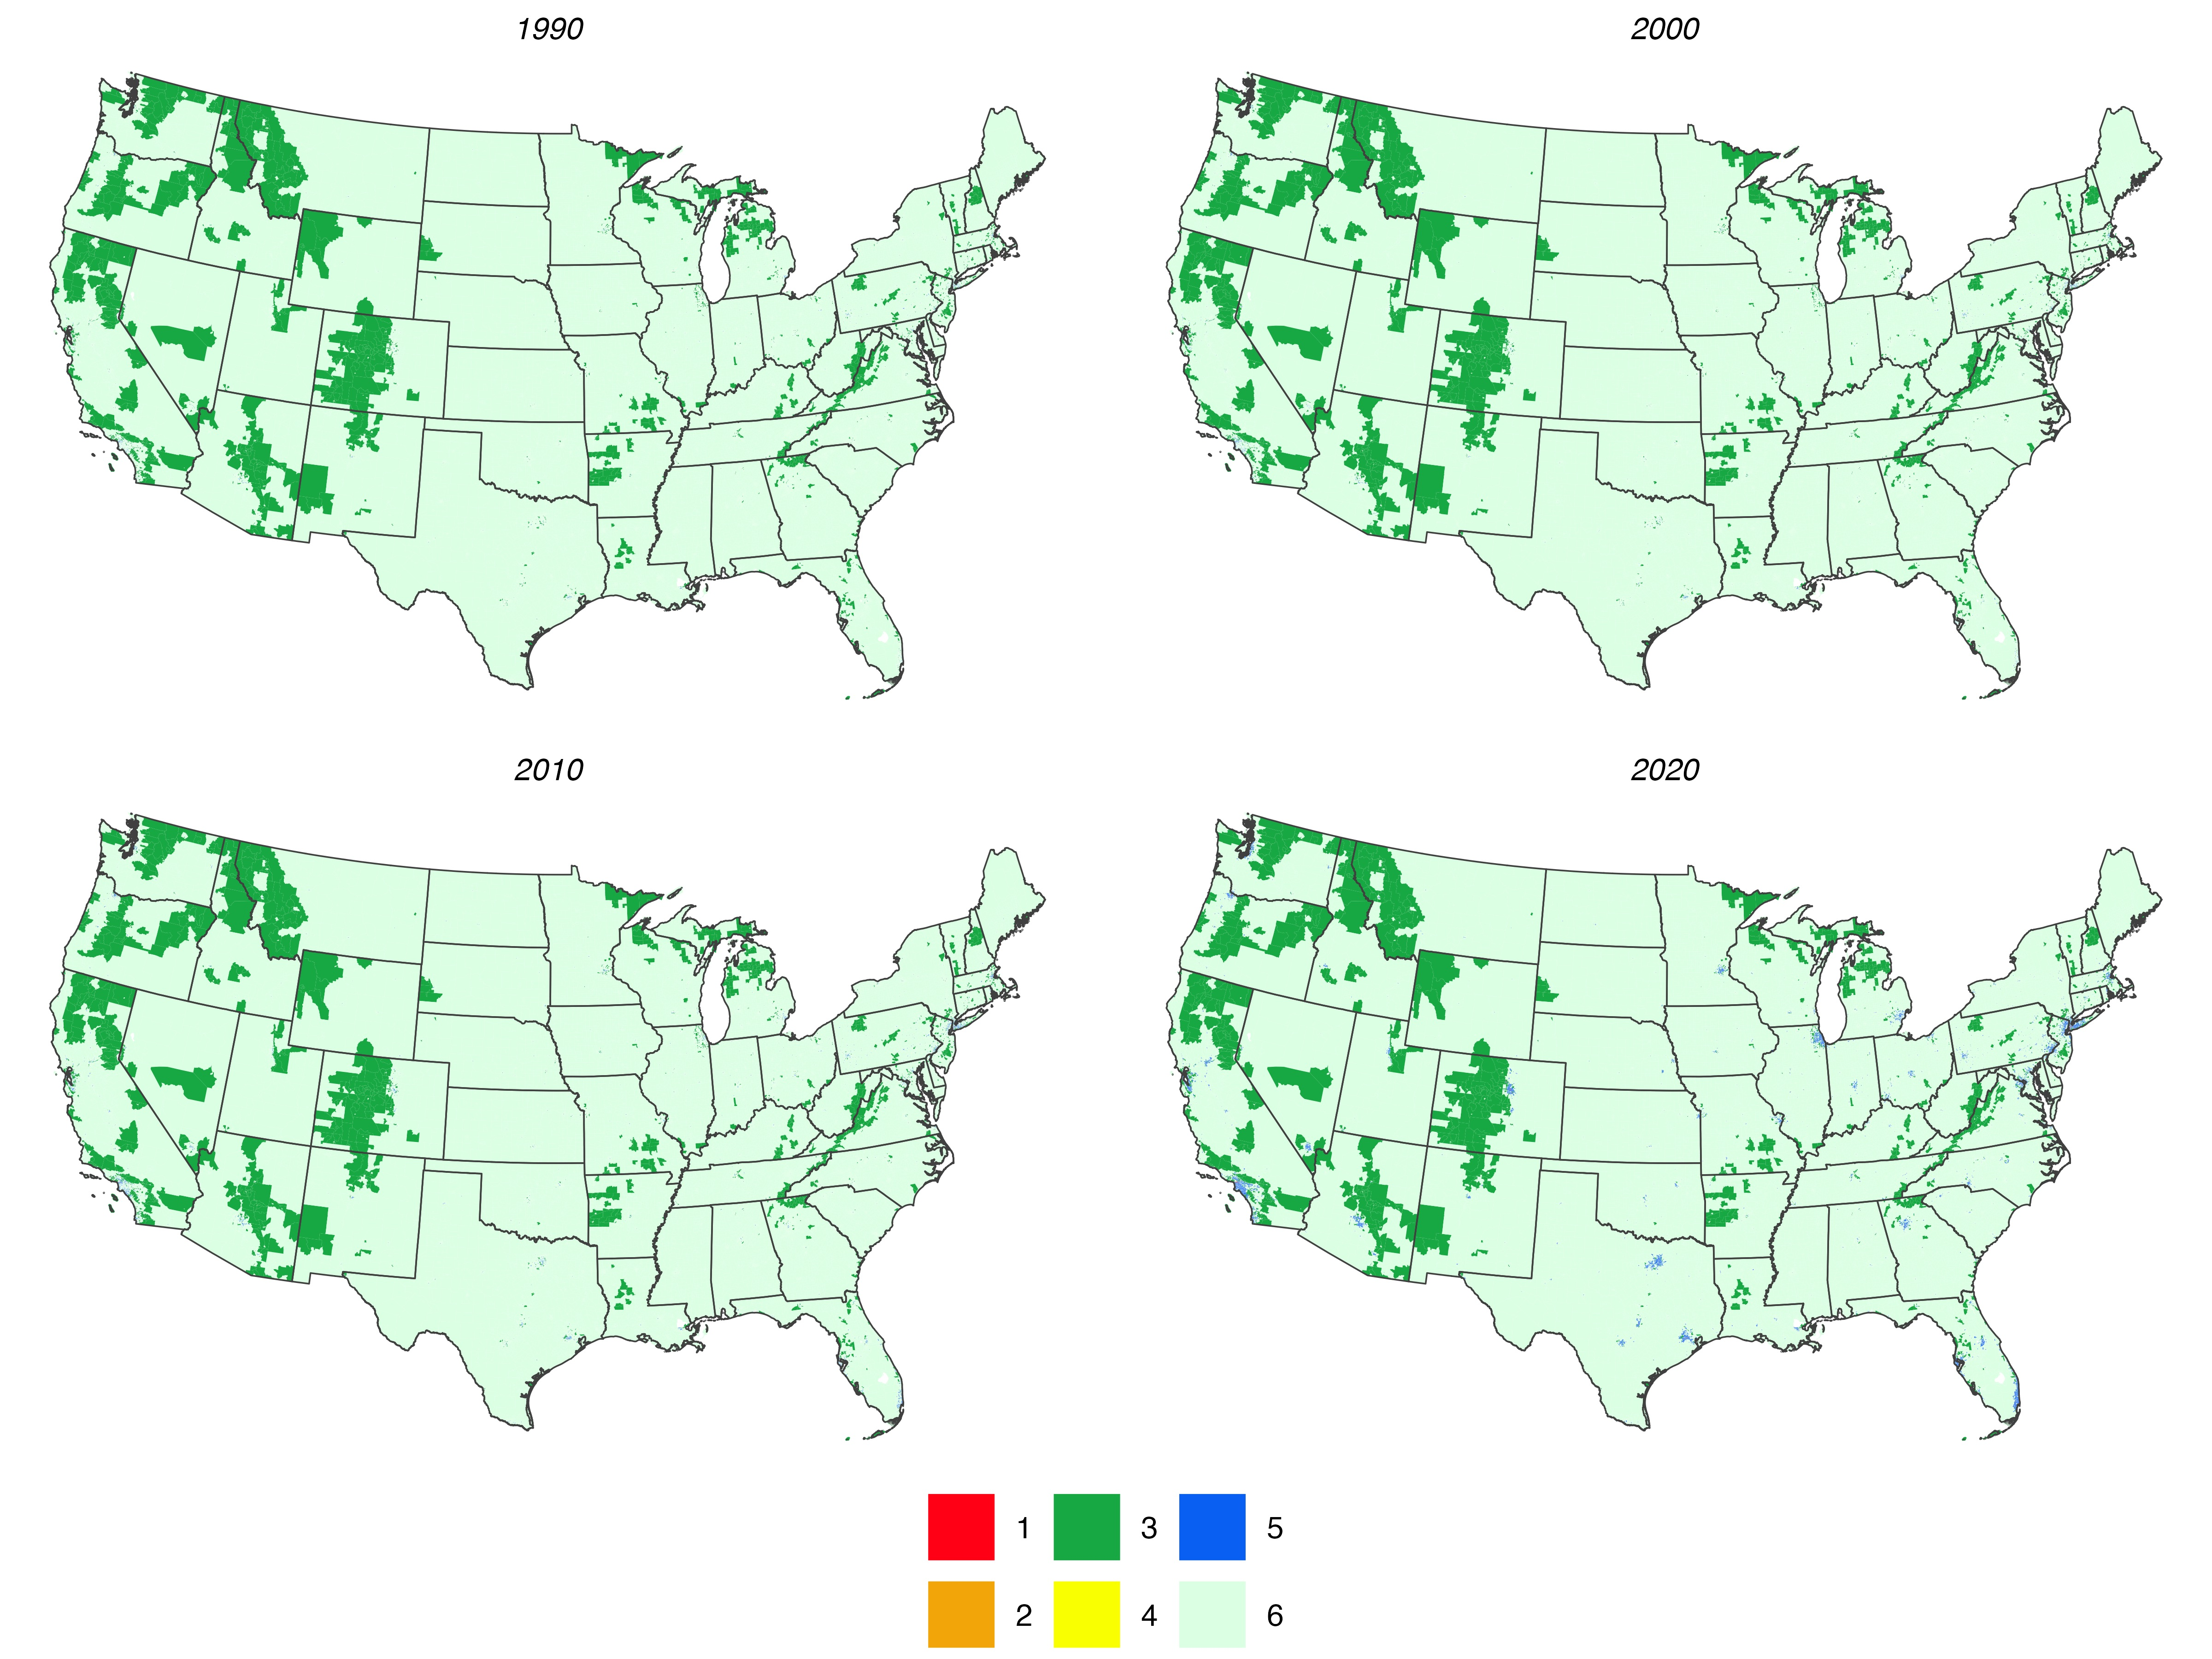
\includegraphics[width=0.75\textwidth,height=\textheight]{imgs/clusters.png}

\hypertarget{geographic-visualization-ord}{%
\section{Geographic Visualization:
ORD}\label{geographic-visualization-ord}}

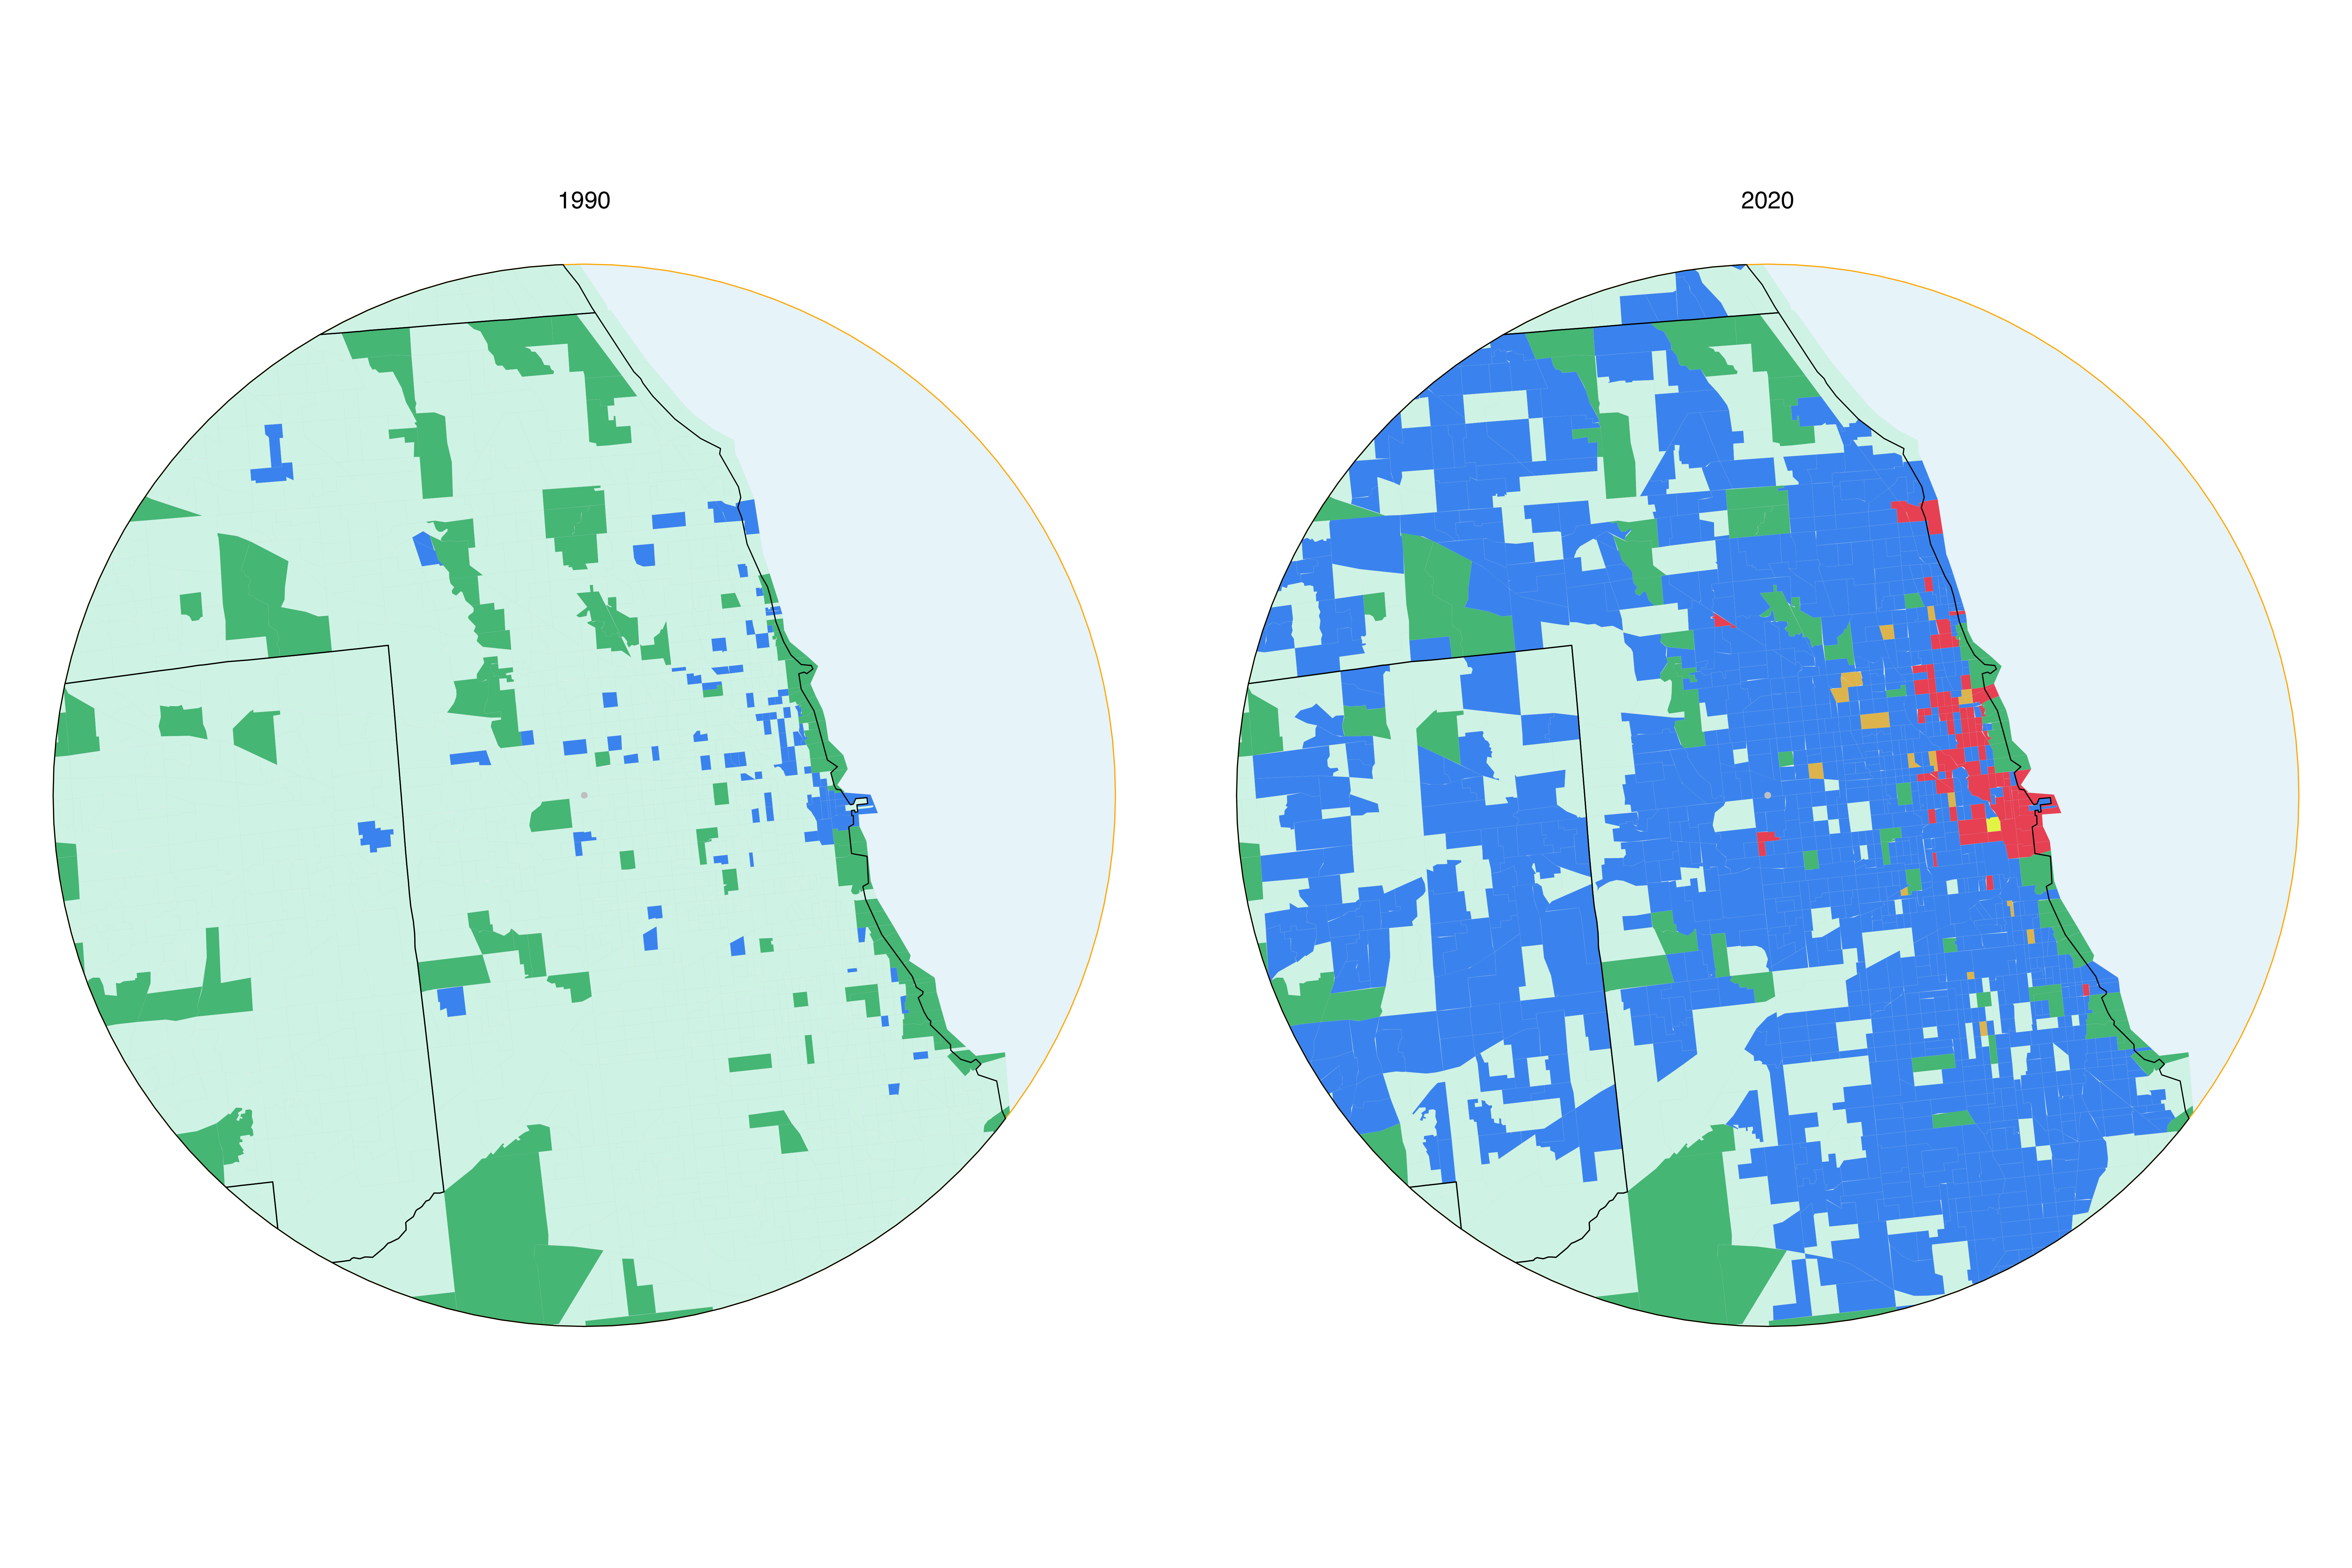
\includegraphics[width=0.7\textwidth,height=\textheight]{imgs/ORD.png}

\hypertarget{geographic-visualization-pdx}{%
\section{Geographic Visualization:
PDX}\label{geographic-visualization-pdx}}

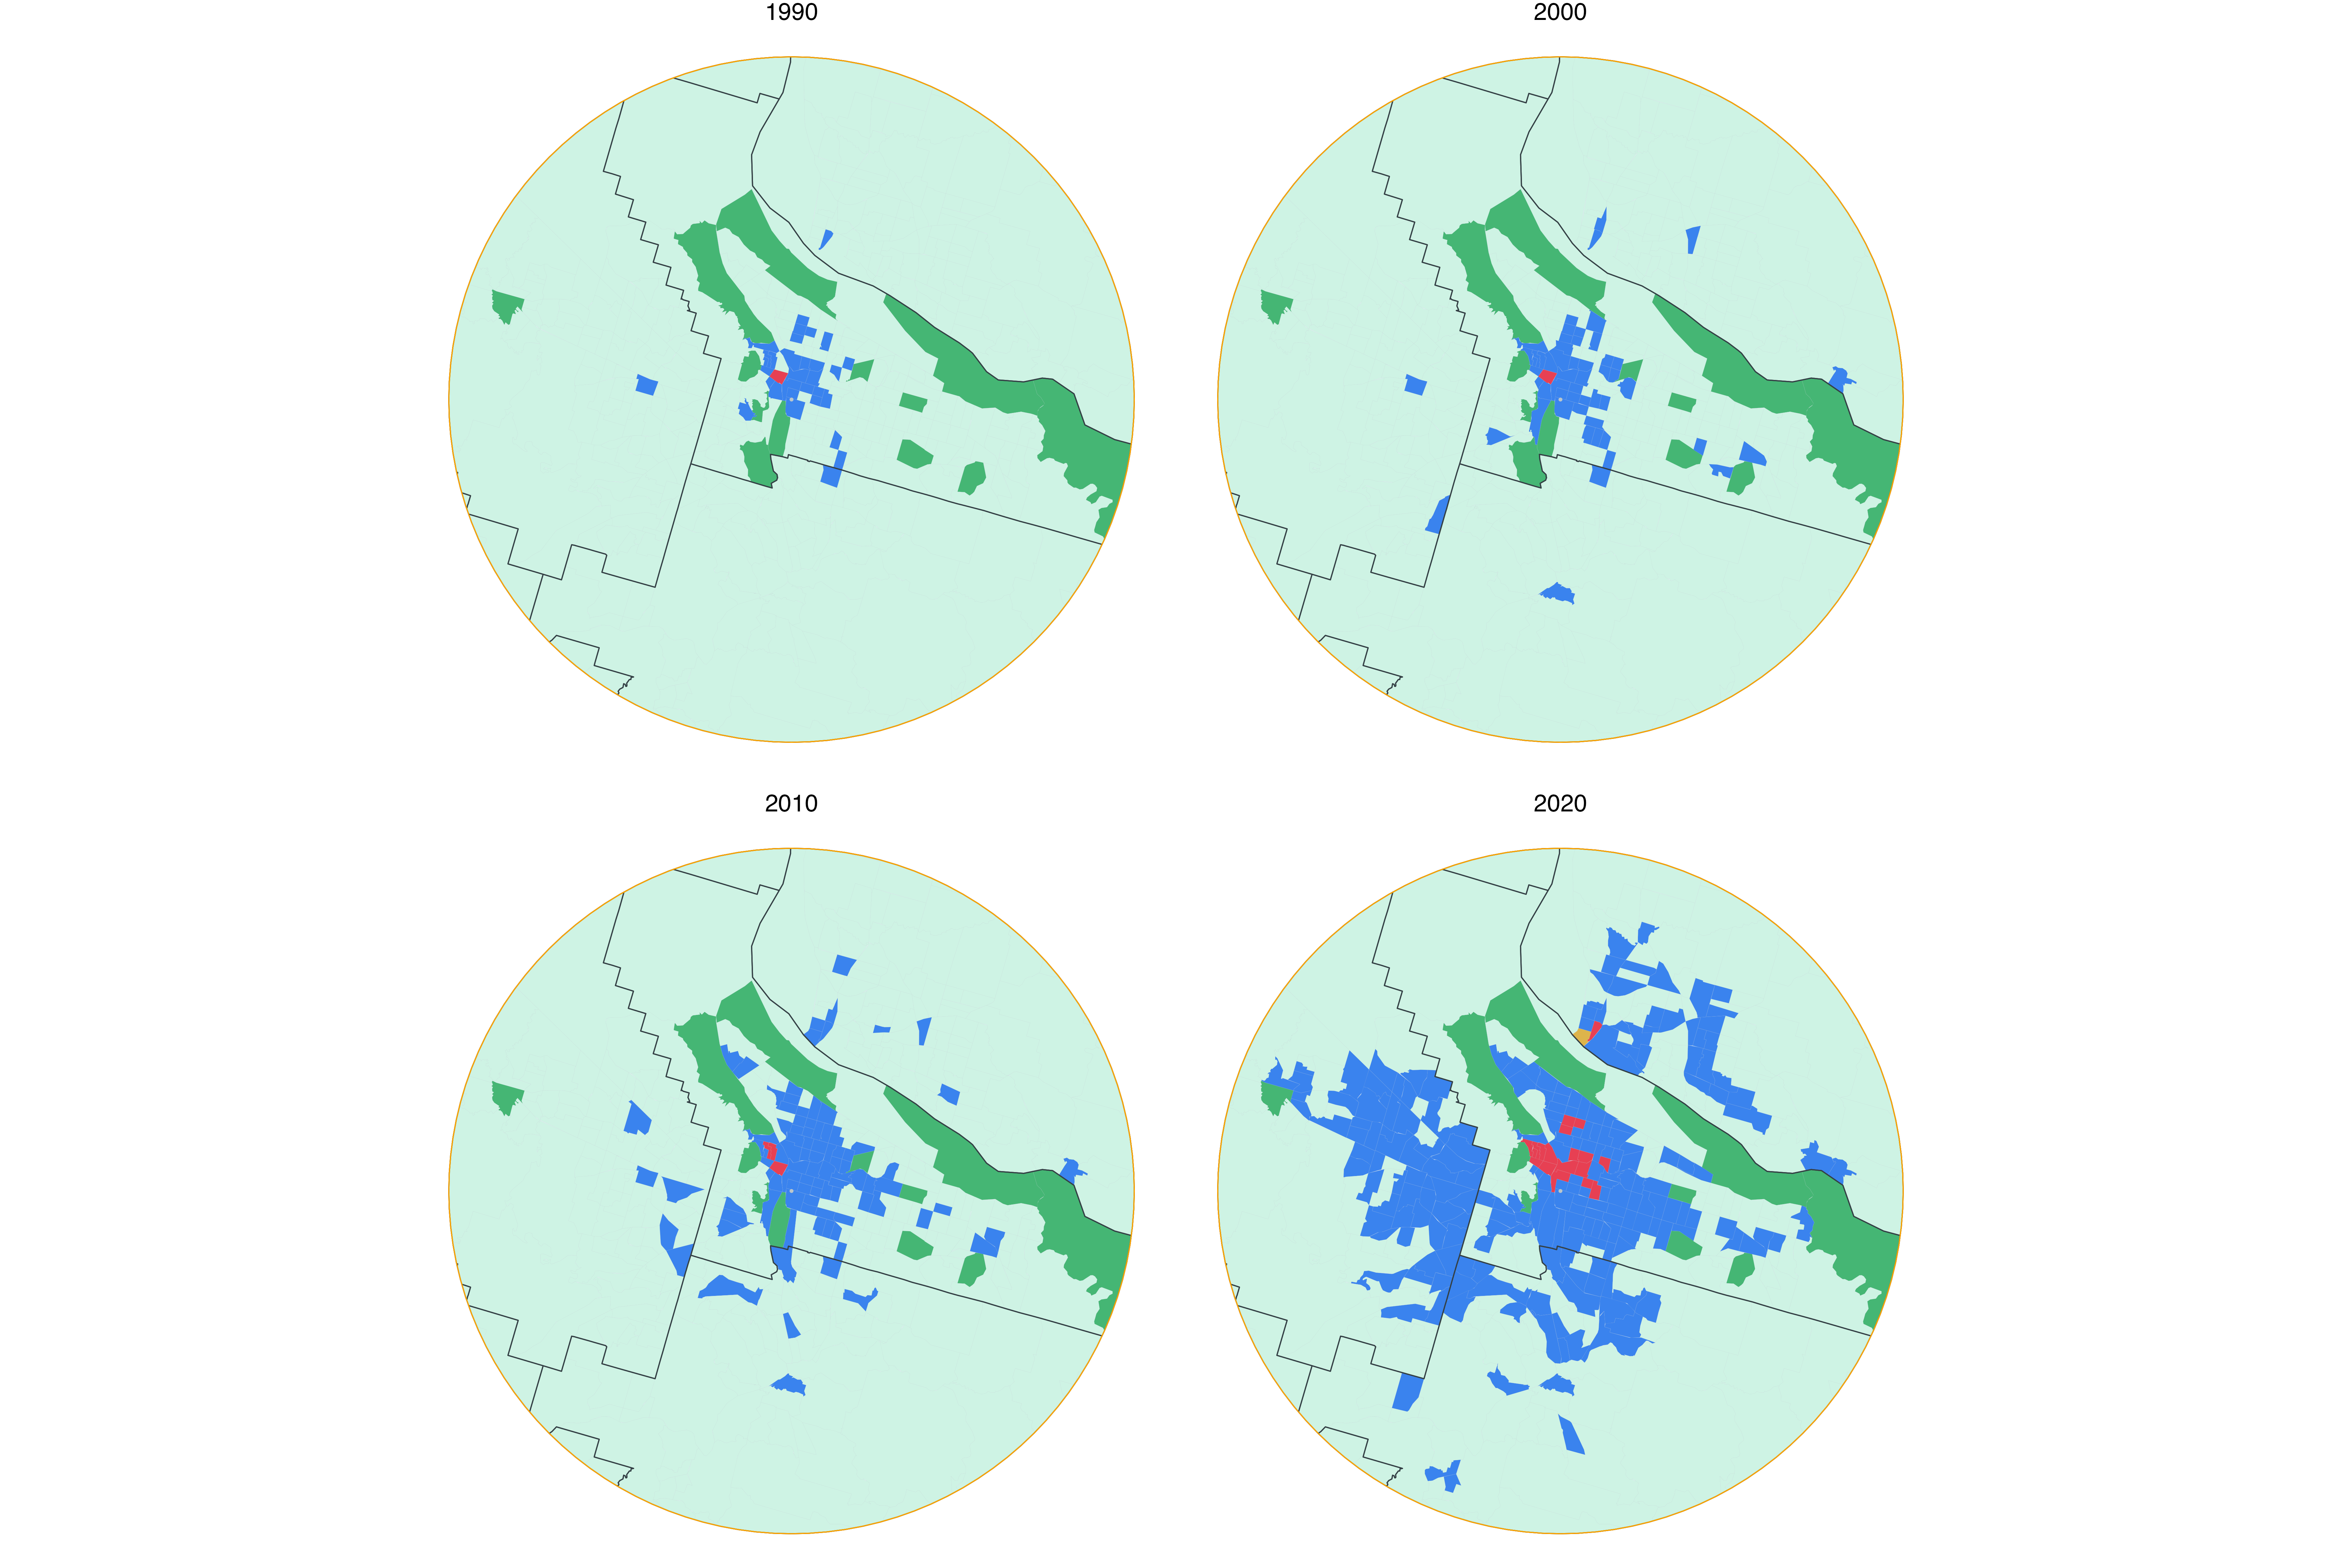
\includegraphics[width=0.7\textwidth,height=\textheight]{imgs/PDX.png}

\hypertarget{geographic-visualization-nyc}{%
\section{Geographic Visualization:
NYC}\label{geographic-visualization-nyc}}

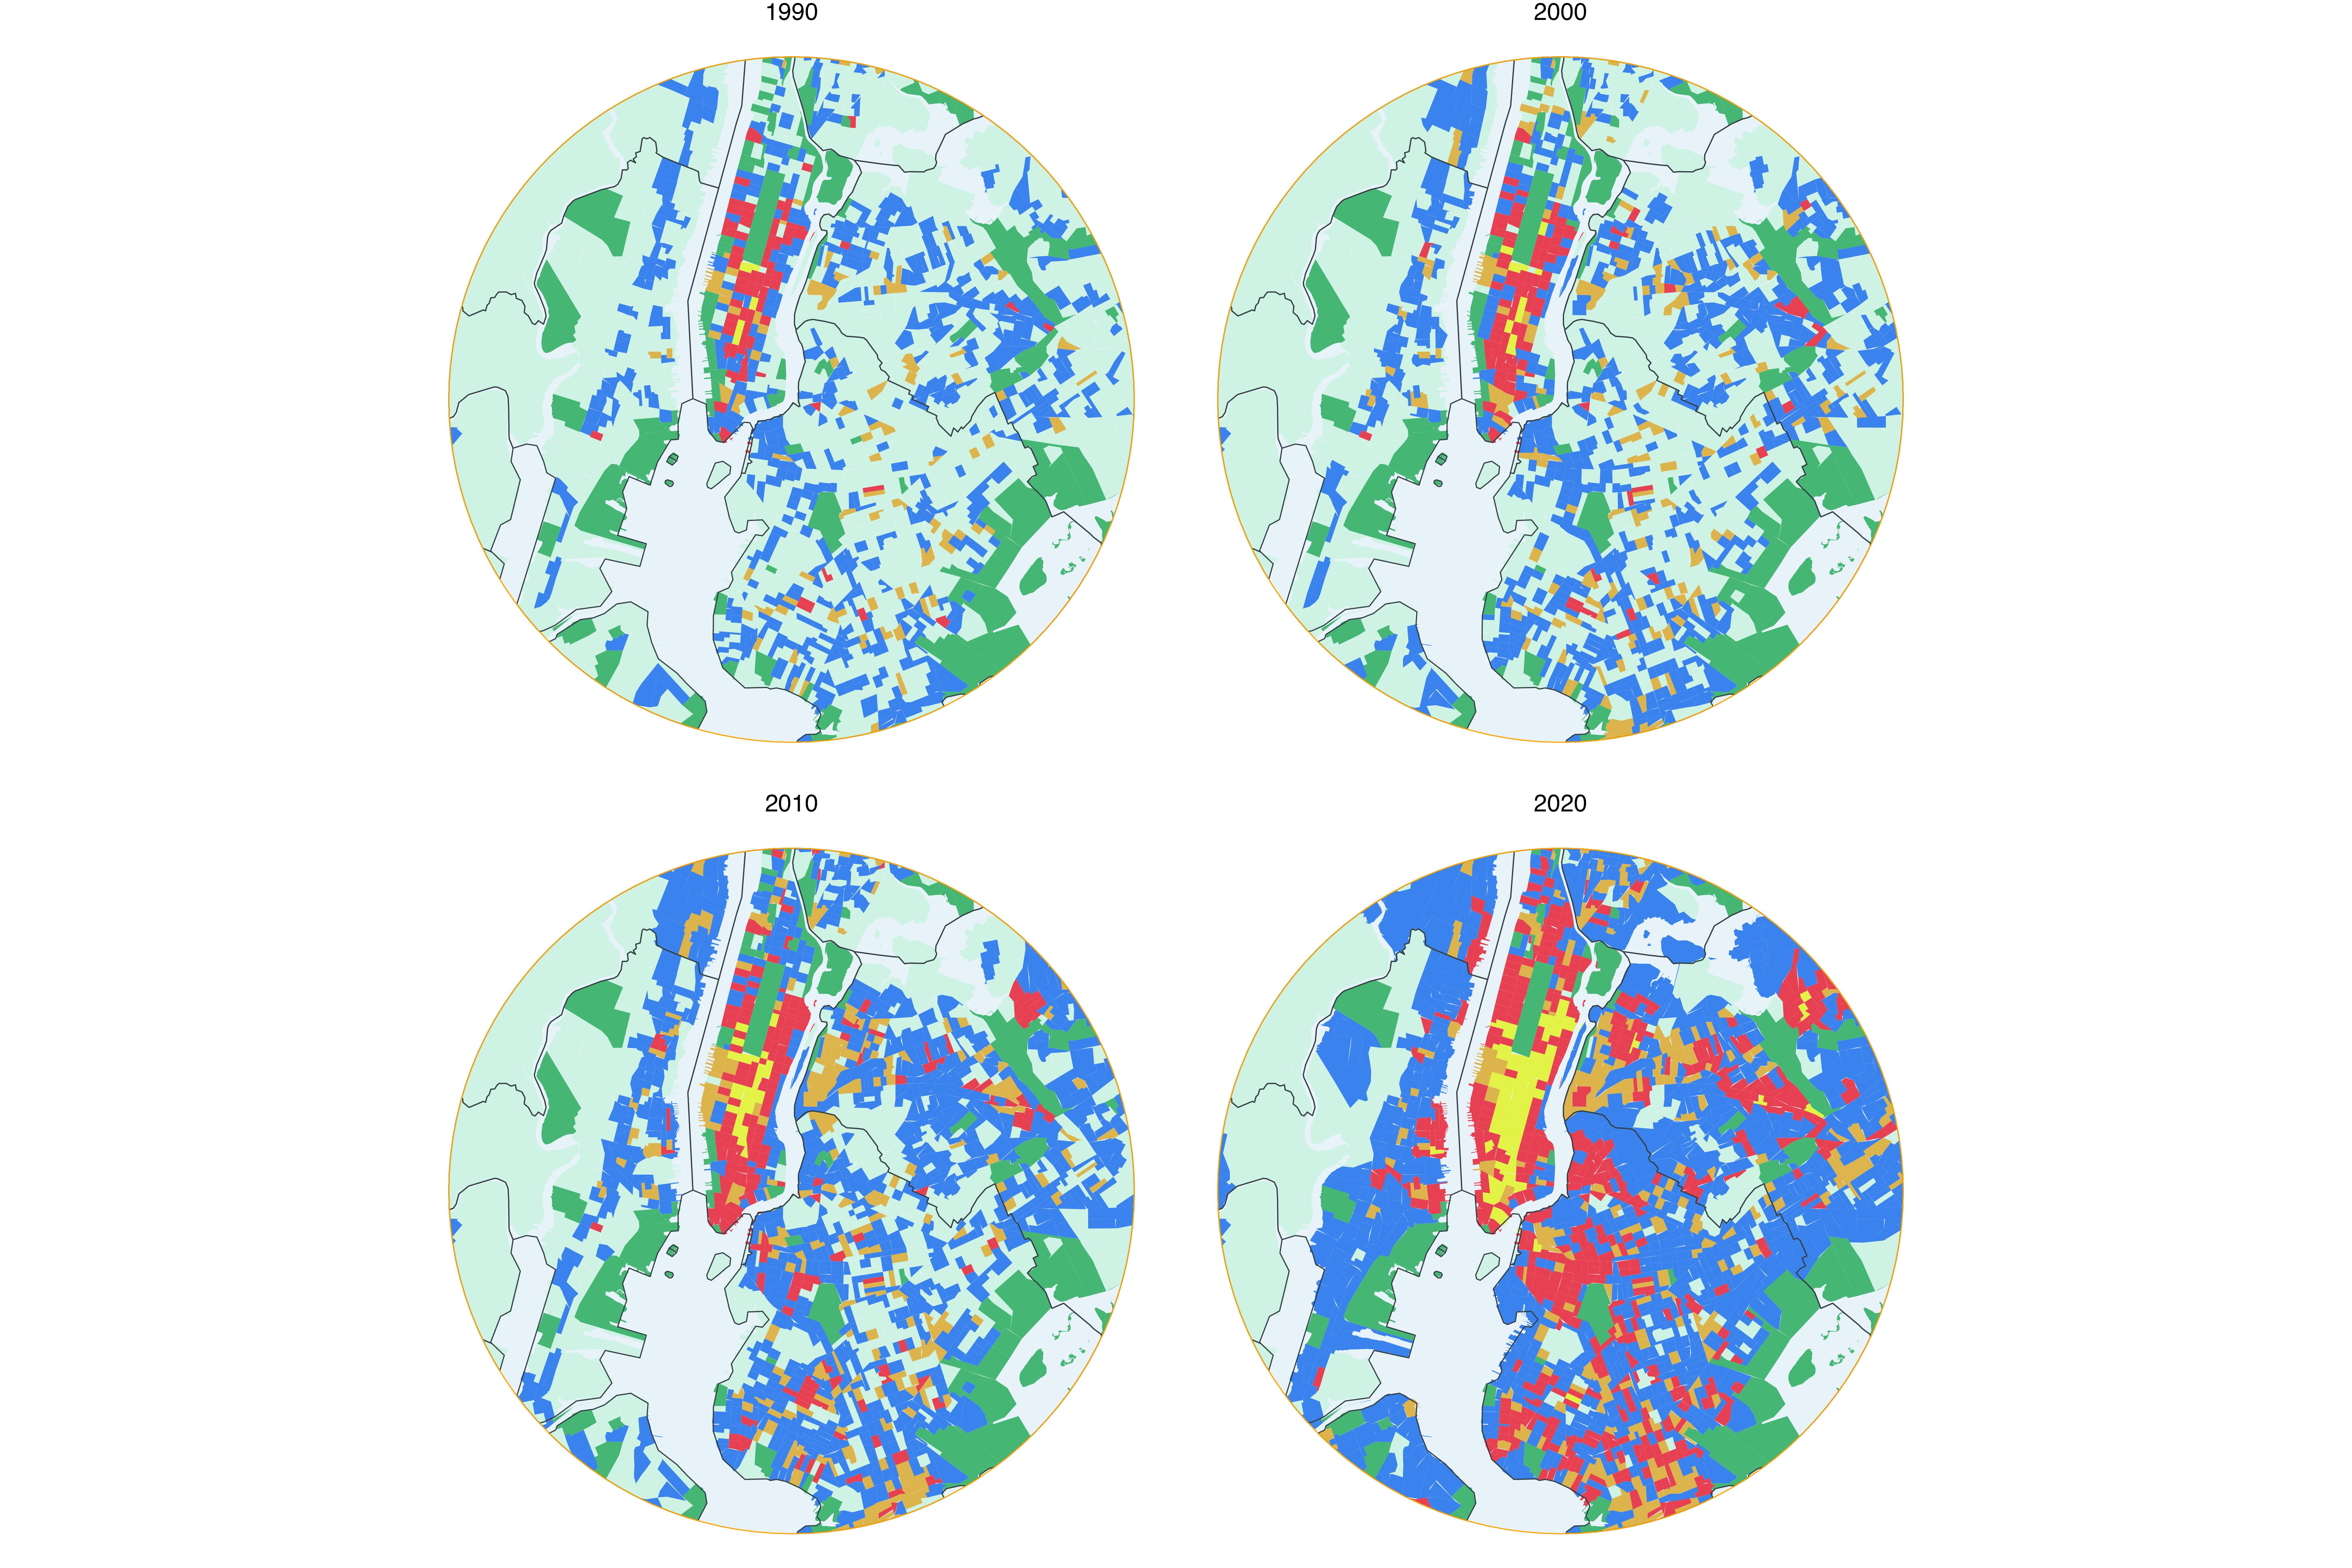
\includegraphics[width=0.7\textwidth,height=\textheight]{imgs/NYC.png}

\hypertarget{geographic-visualization-buf}{%
\section{Geographic Visualization:
BUF}\label{geographic-visualization-buf}}

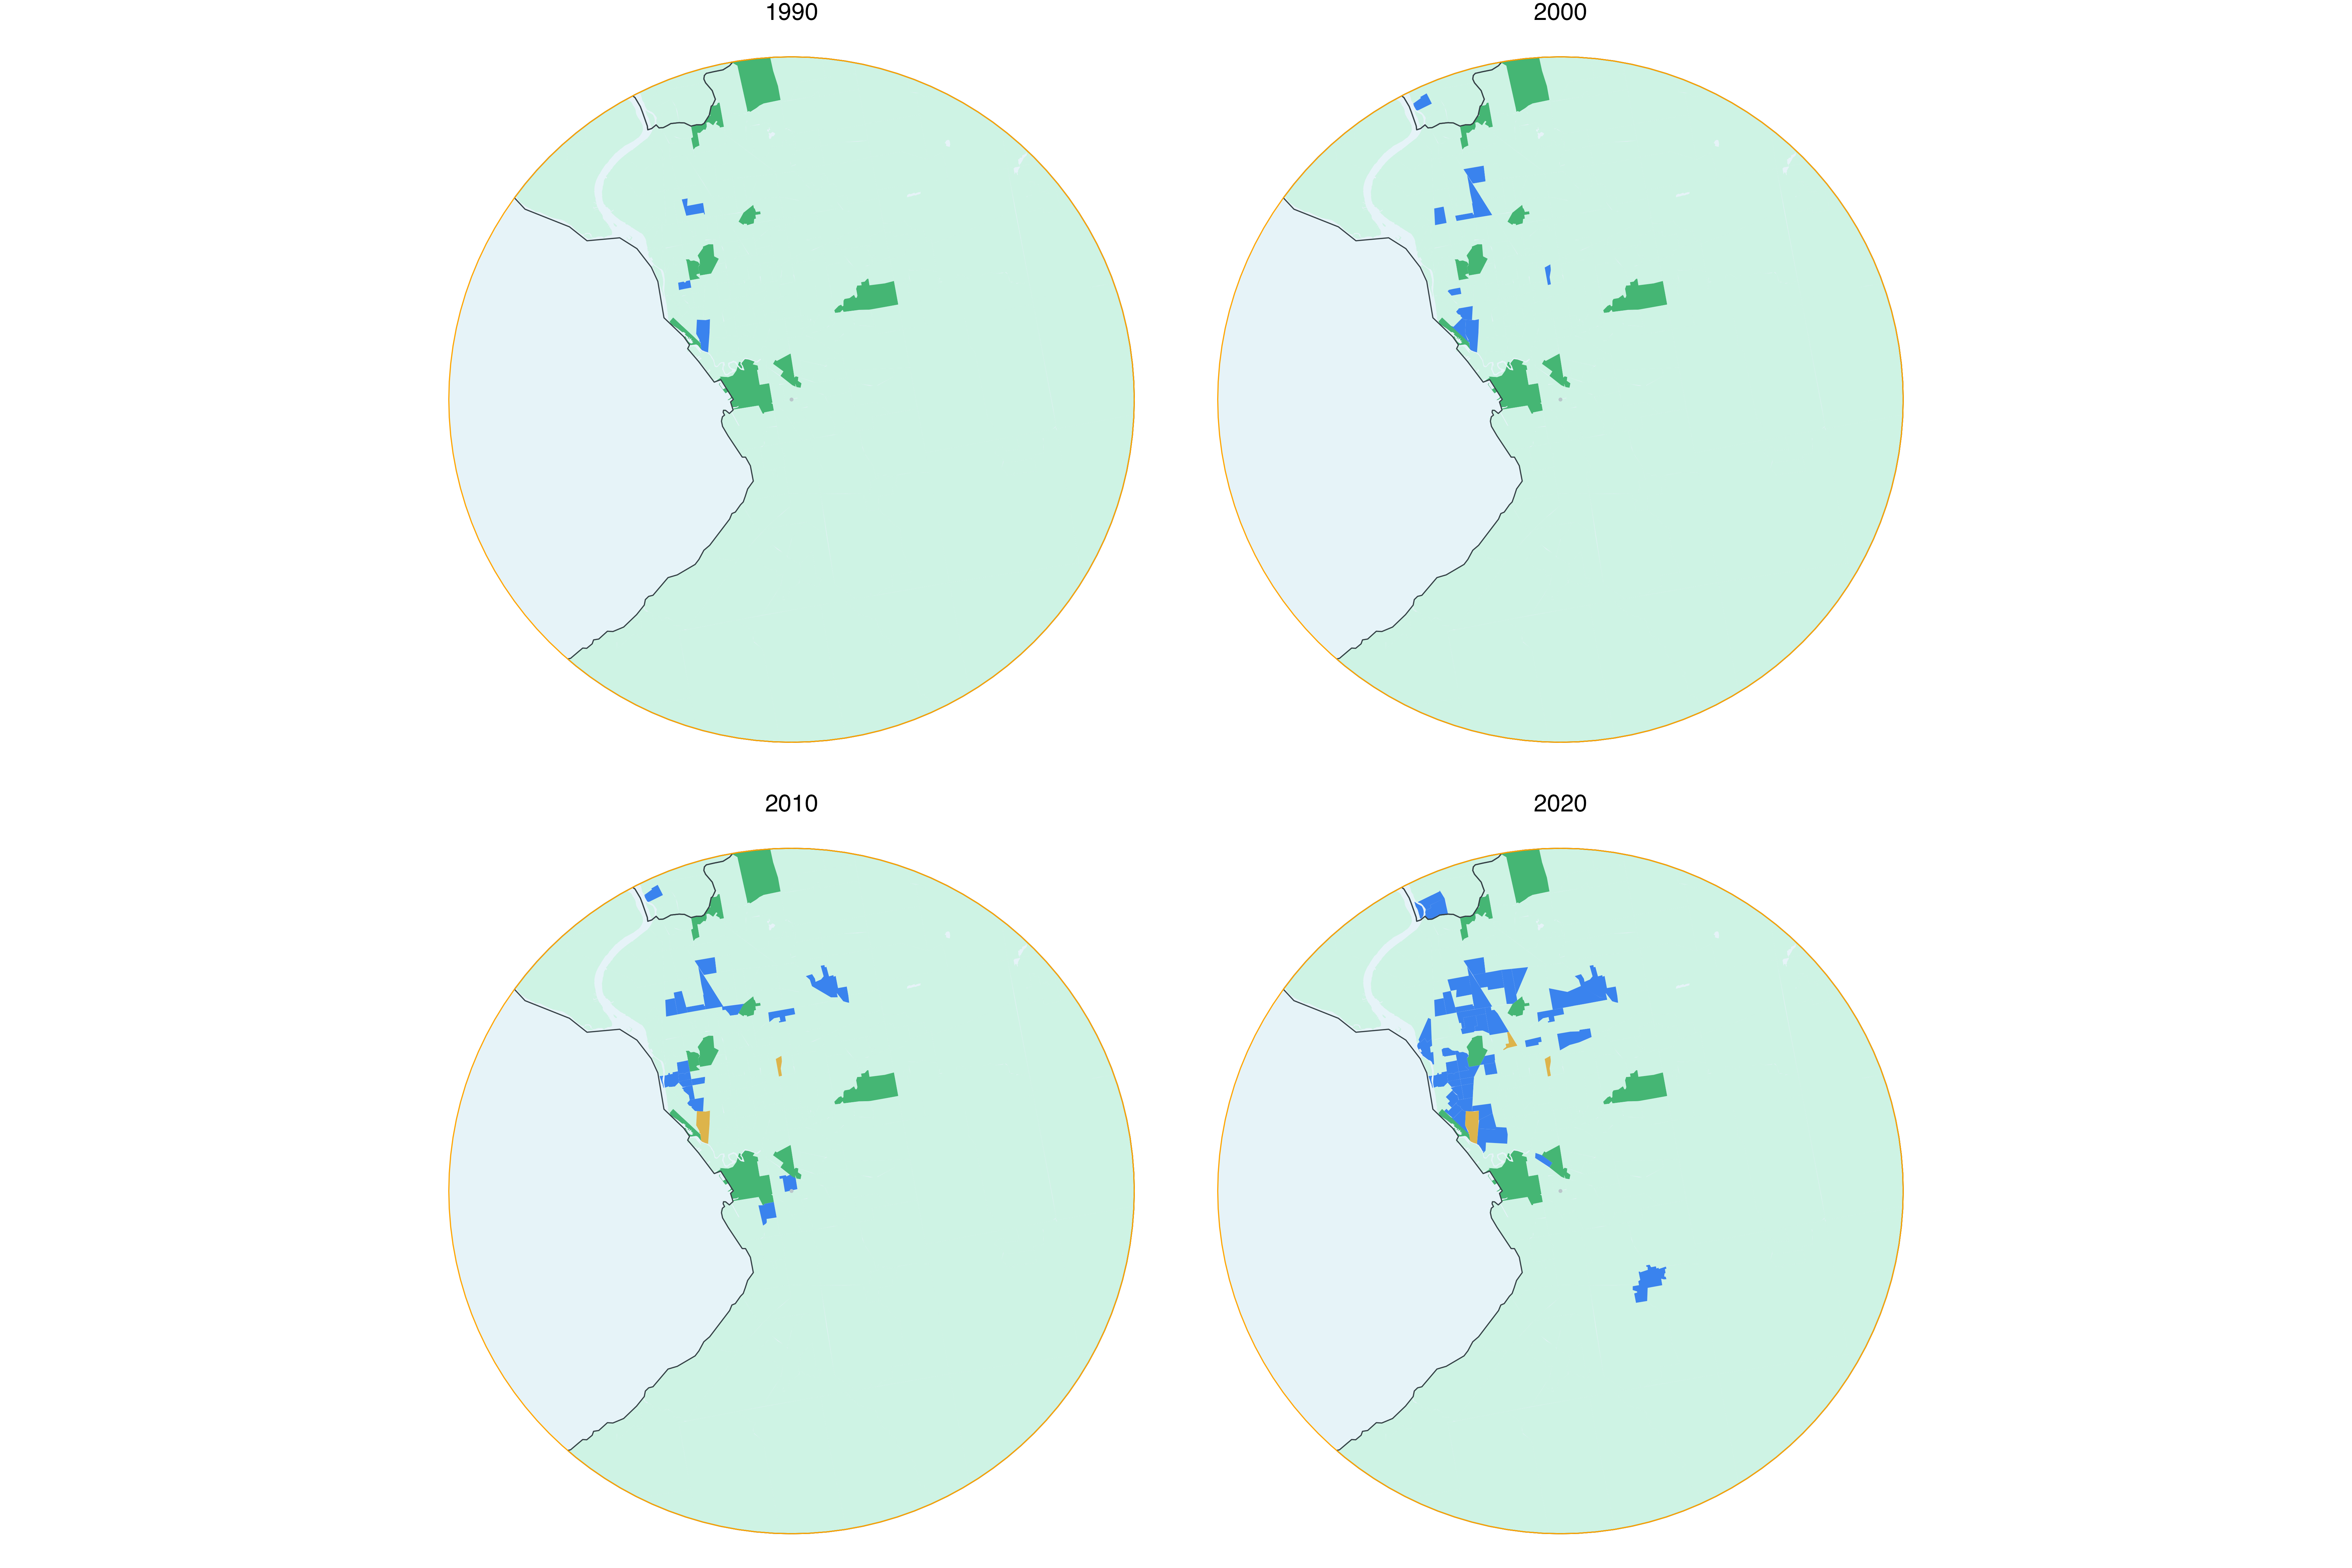
\includegraphics[width=0.7\textwidth,height=\textheight]{imgs/BUF.png}

\hypertarget{geographic-visualization-dtw}{%
\section{Geographic Visualization:
DTW}\label{geographic-visualization-dtw}}

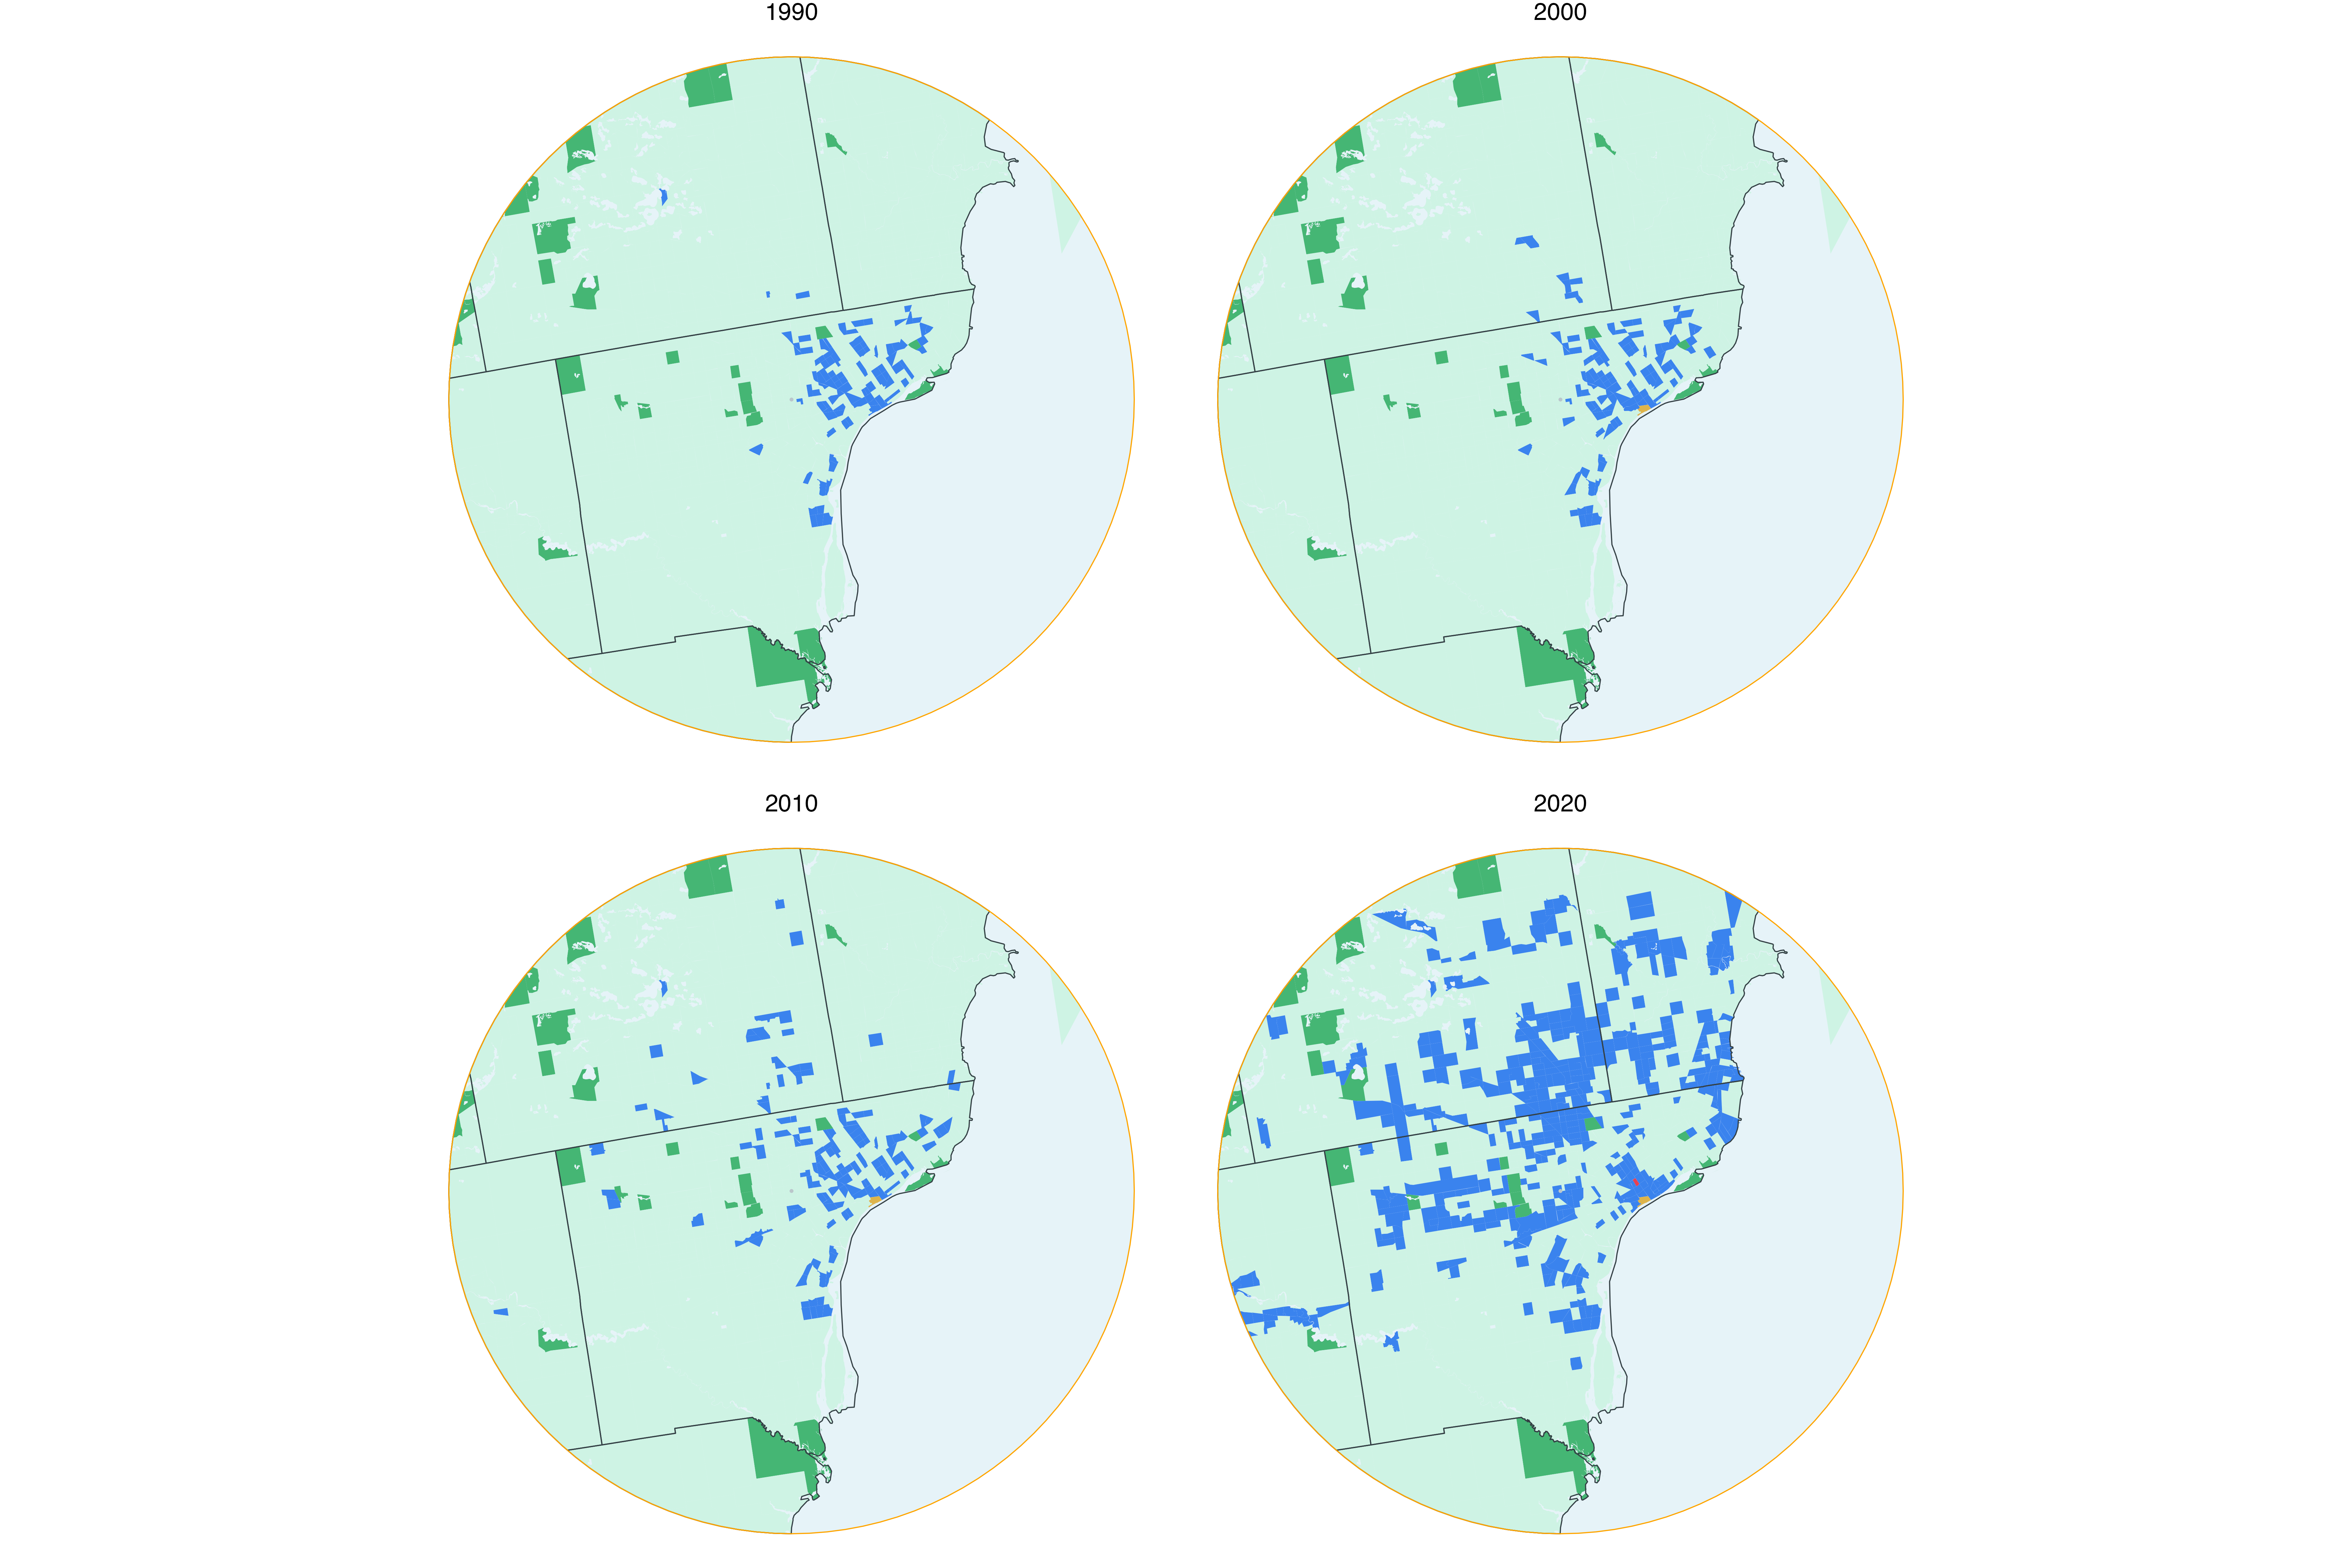
\includegraphics[width=0.7\textwidth,height=\textheight]{imgs/DTW.png}

\hypertarget{geographic-visualization-villages}{%
\section{Geographic Visualization:
Villages}\label{geographic-visualization-villages}}

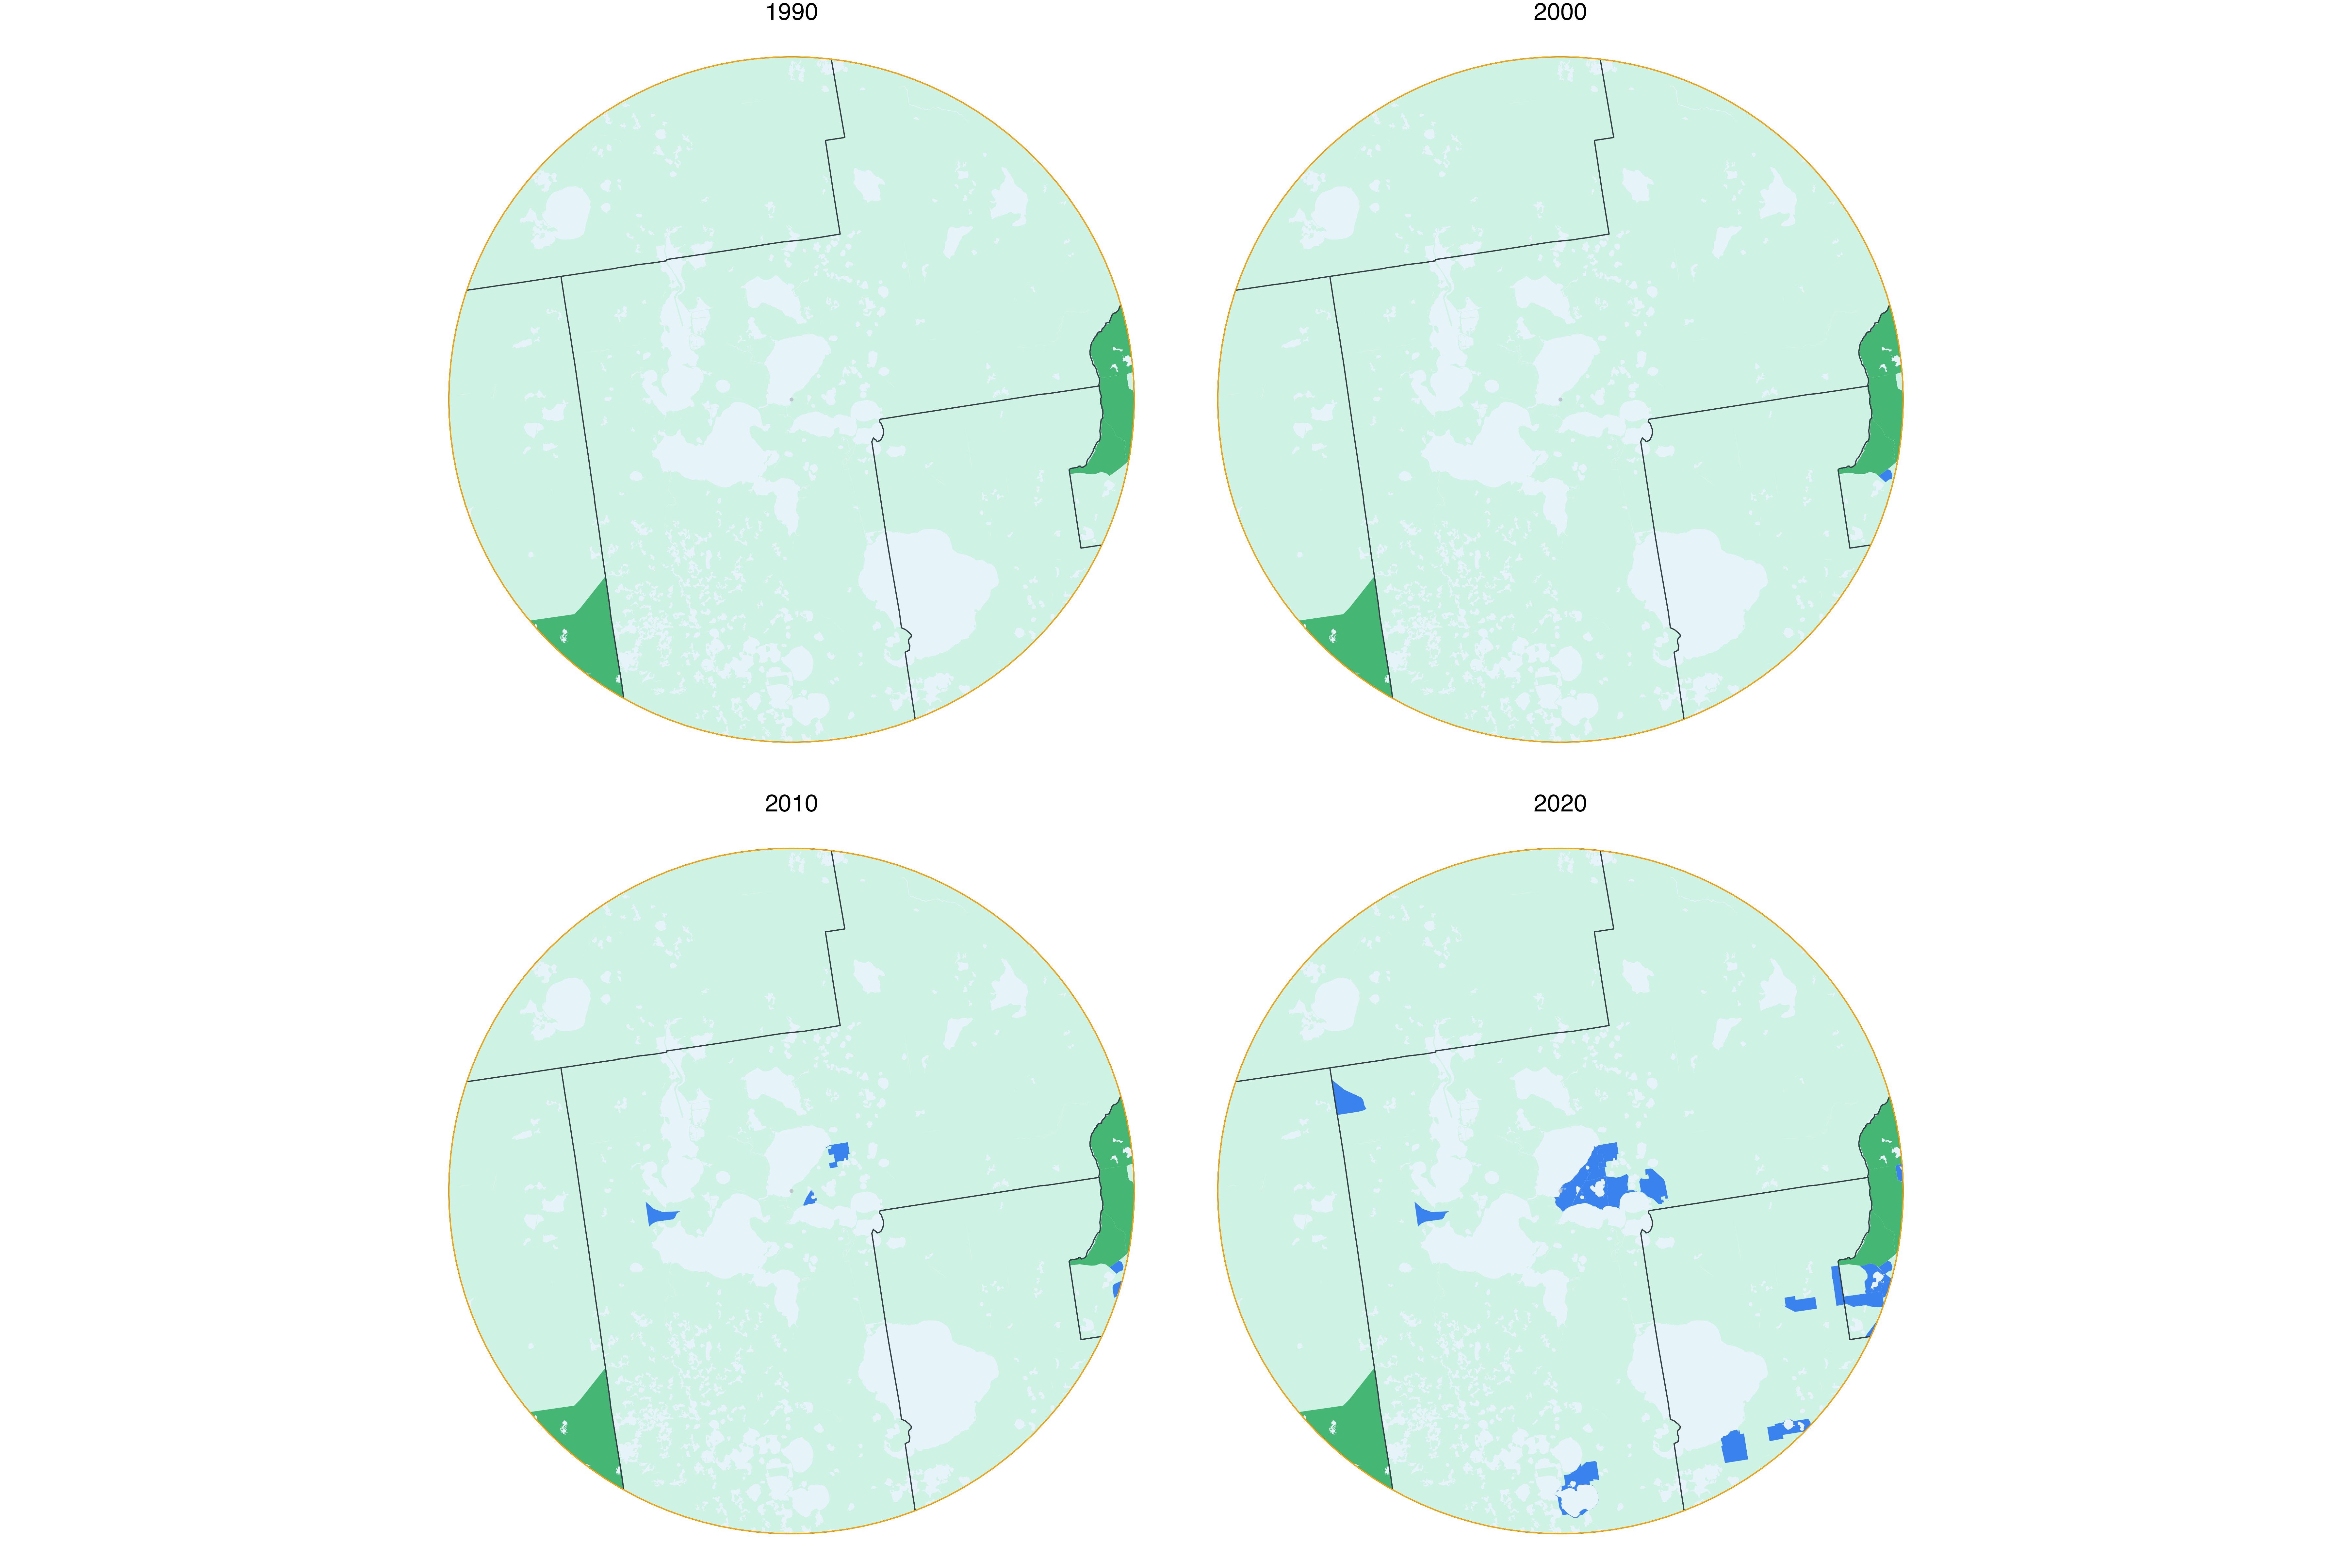
\includegraphics[width=0.7\textwidth,height=\textheight]{imgs/VIL.png}

\hypertarget{geographic-visualization-phl}{%
\section{Geographic Visualization:
PHL}\label{geographic-visualization-phl}}

\includegraphics[width=0.7\textwidth,height=\textheight]{imgs/PHL.png}

\hypertarget{changing-clusters-1}{%
\section{Changing clusters (1)}\label{changing-clusters-1}}

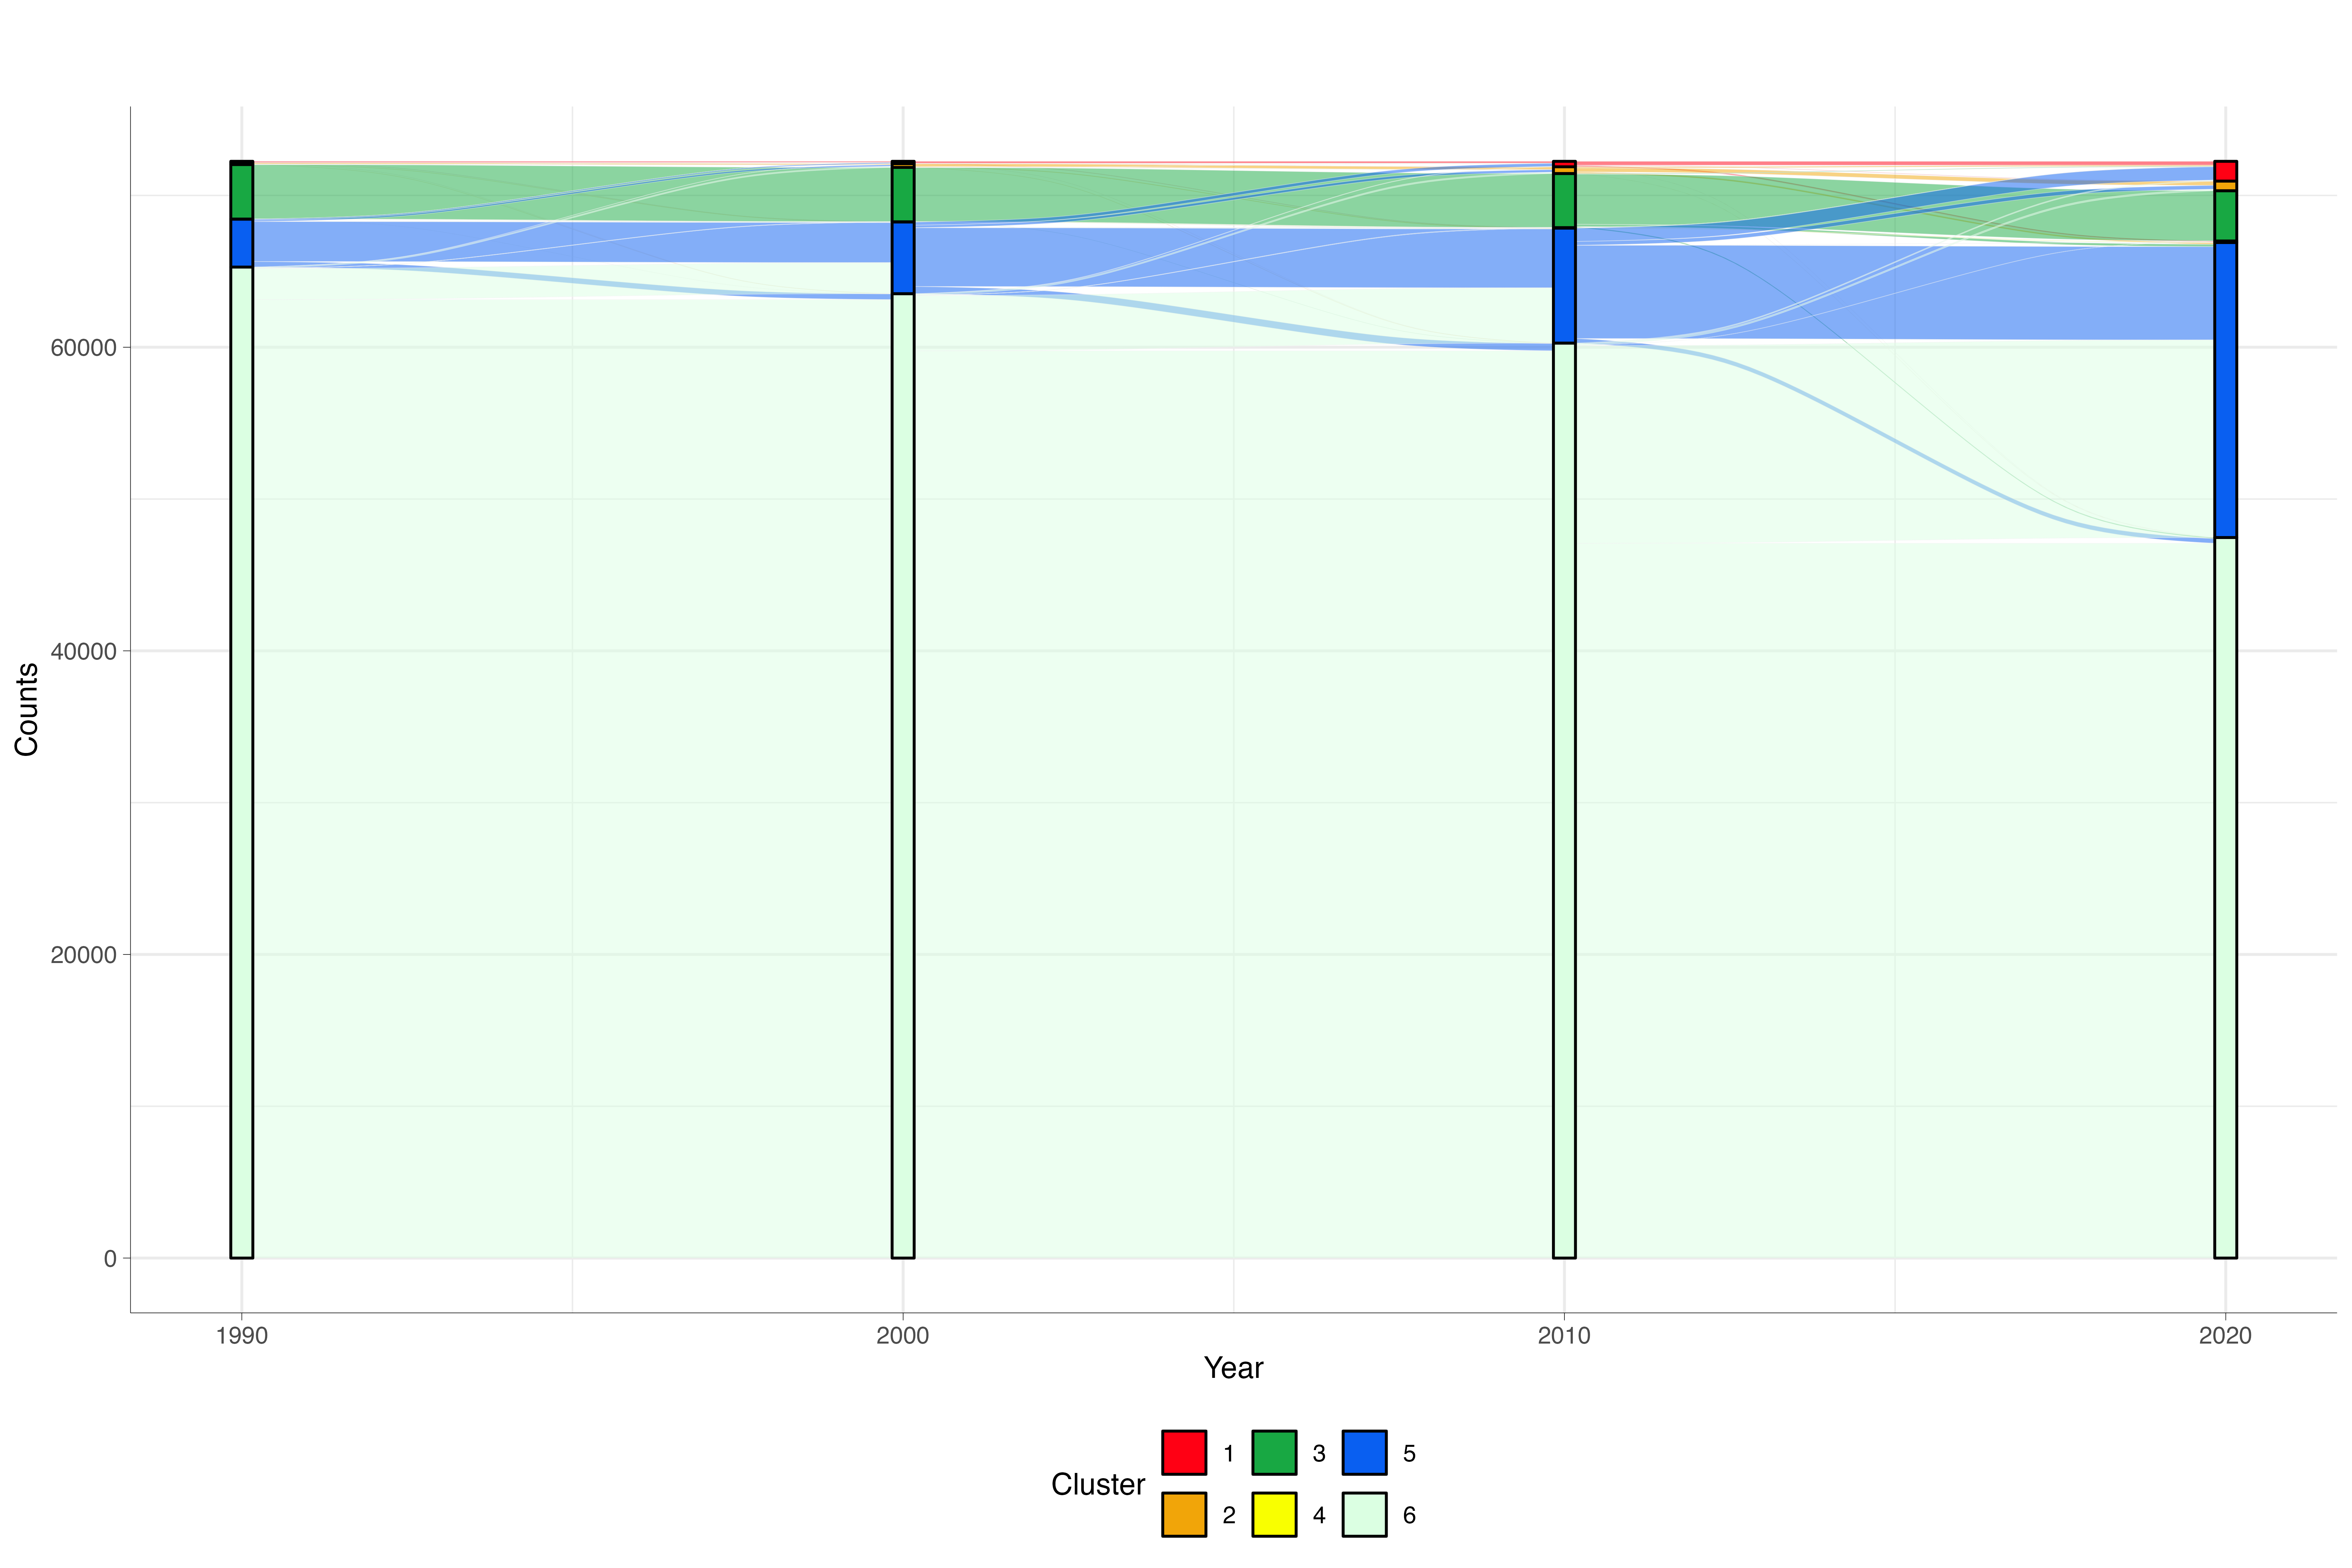
\includegraphics[width=0.7\textwidth,height=\textheight]{imgs/sankey.png}

\hypertarget{changing-clusters-2}{%
\section{Changing clusters (2)}\label{changing-clusters-2}}

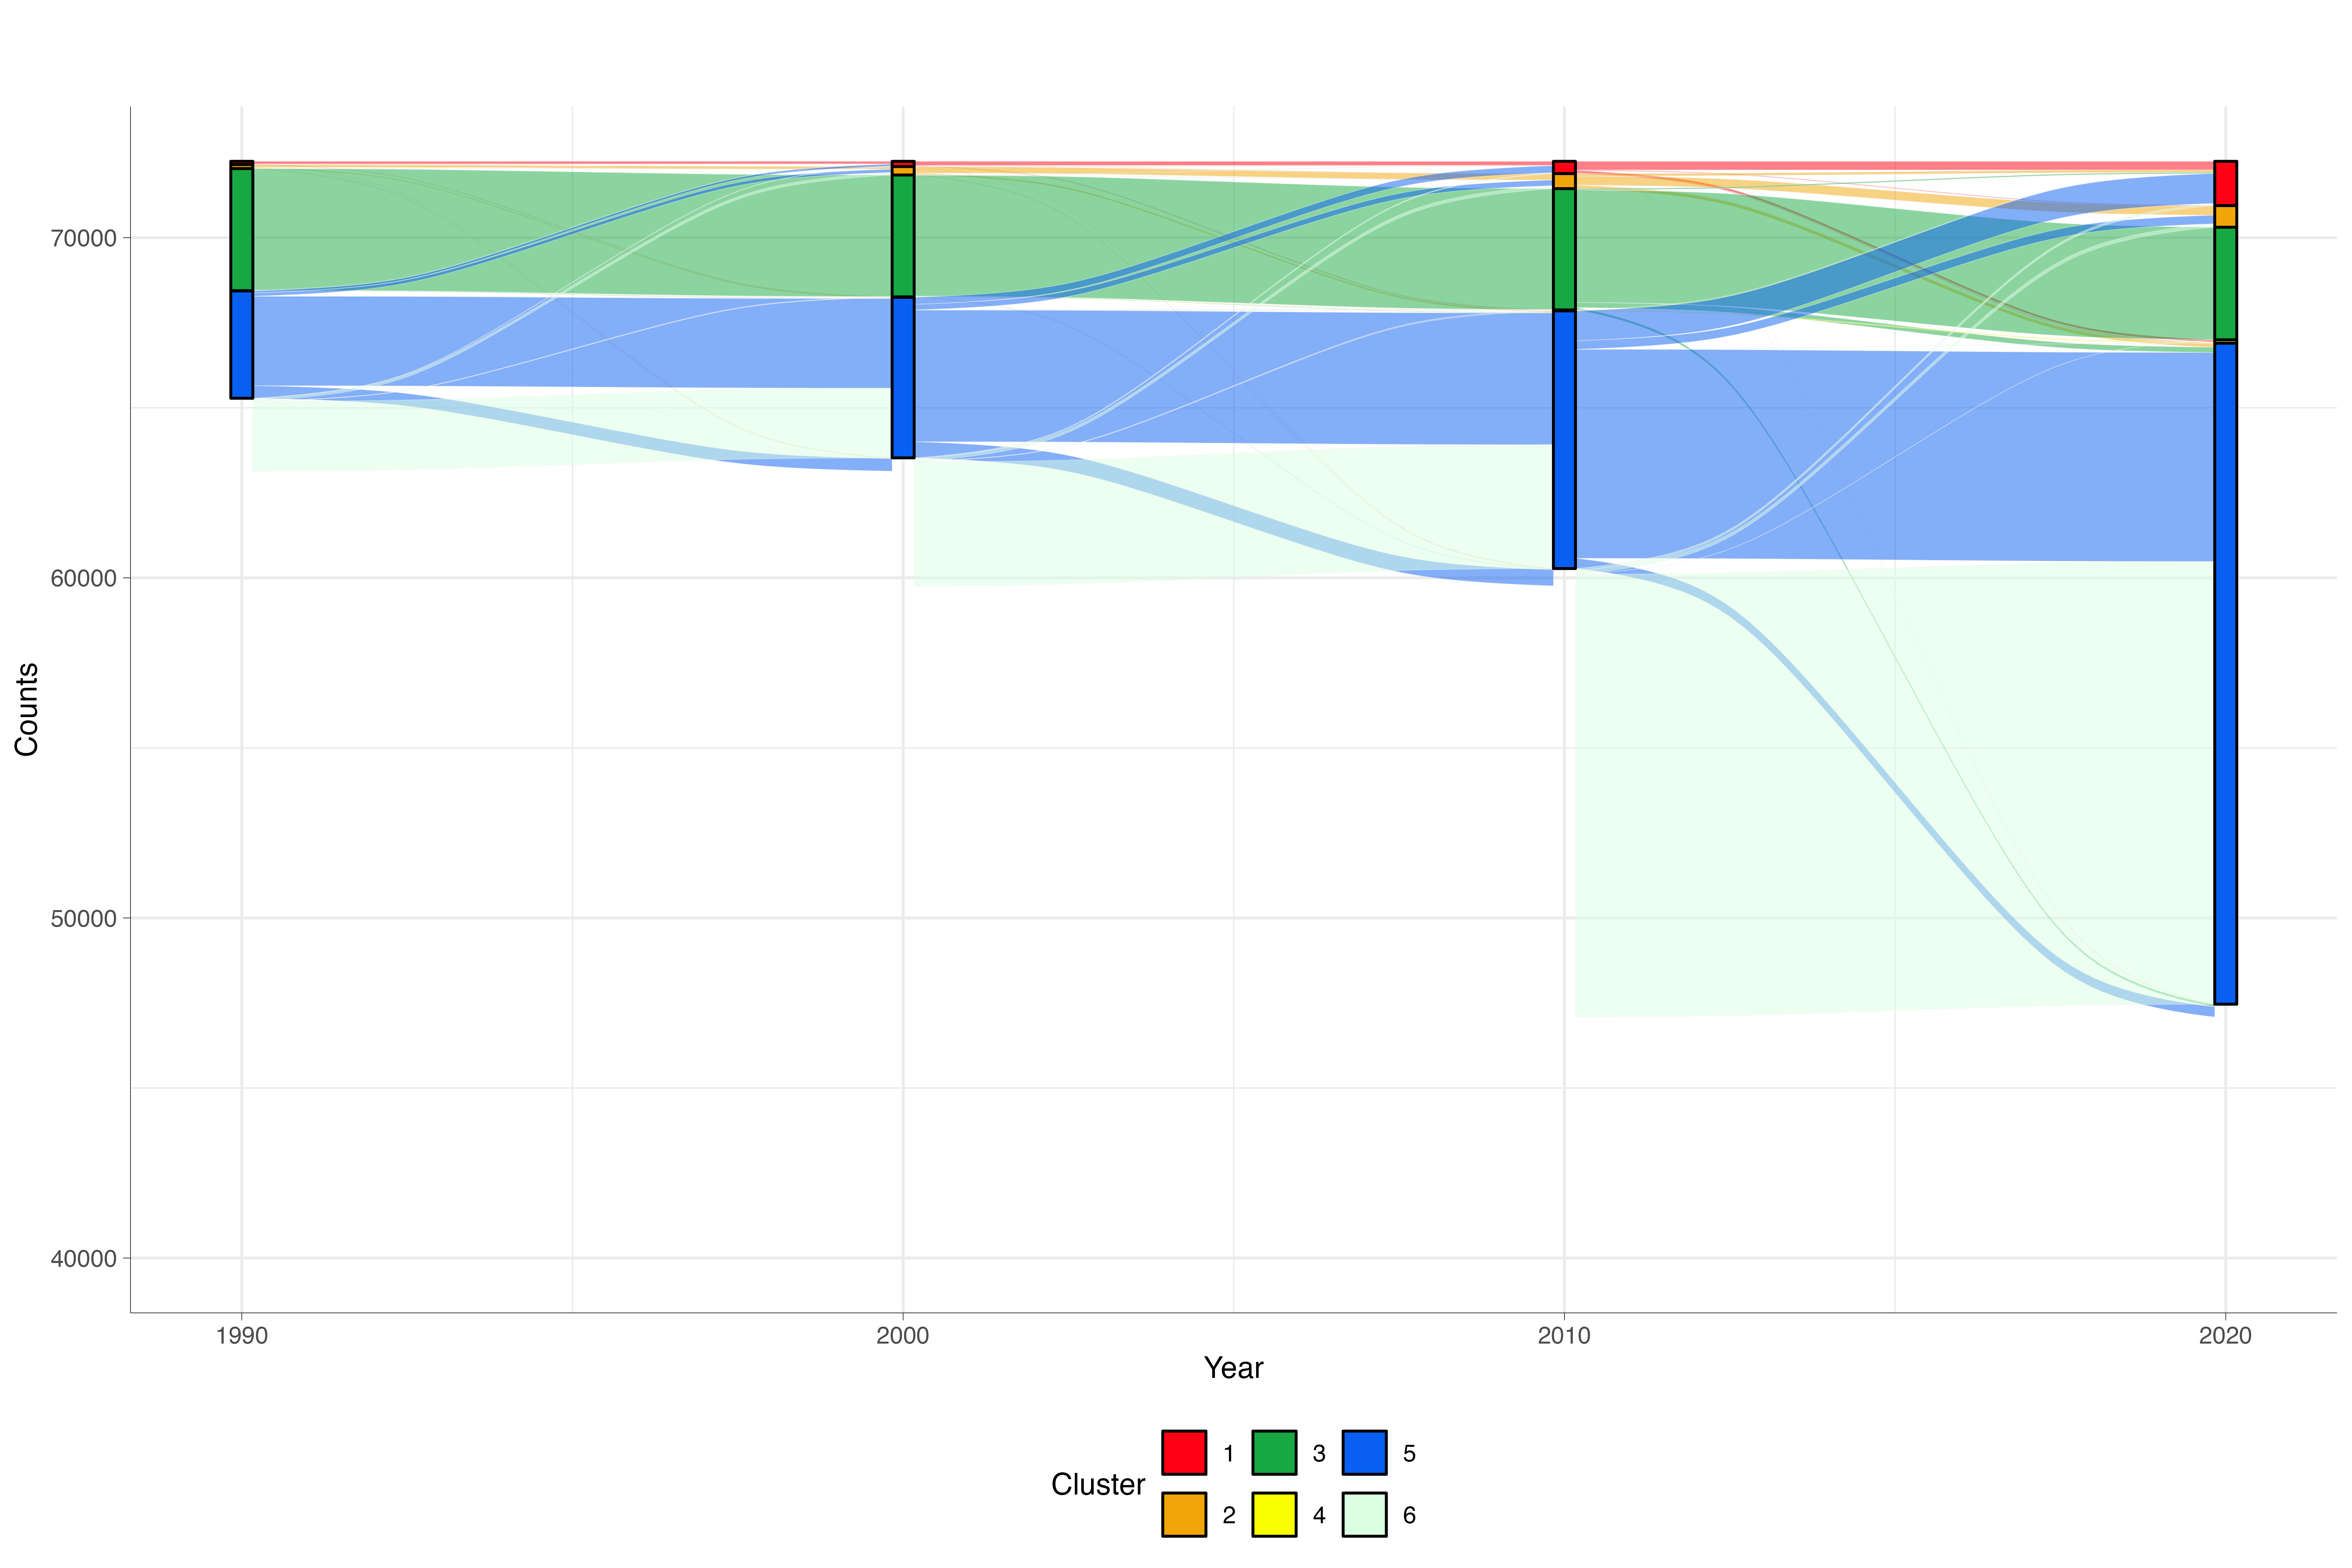
\includegraphics[width=0.7\textwidth,height=\textheight]{imgs/sankeyB.png}

\hypertarget{preliminary-observations-12}{%
\section{Preliminary observations
(1/2)}\label{preliminary-observations-12}}

\begin{itemize}
\tightlist
\item
  A strong group of census tracts remain in the same cluster

  \begin{itemize}
  \tightlist
  \item
    rural, but rapidly giving space to residential suburbs
  \end{itemize}
\item
  Cities tend to see a more diverse set of clusters

  \begin{itemize}
  \tightlist
  \item
    clusters are much smaller
  \end{itemize}
\end{itemize}

\hypertarget{preliminary-observations-22}{%
\section{Preliminary observations
(2/2)}\label{preliminary-observations-22}}

\begin{itemize}
\tightlist
\item
  Is our approach valid to characterize ageing communities?
\item
  Are there distinct \textbf{clusters} of neighborhood aging resources?
\item
  Have the resources within \textbf{clusters} changed over time, and
  how?
\end{itemize}

\hypertarget{next-steps}{%
\section{Next steps}\label{next-steps}}

\begin{itemize}
\tightlist
\item
  Data driven \texttt{PCA}
\item
  Associations with demographics factors (paper 2)
\end{itemize}

\hypertarget{timeline}{%
\section{Timeline}\label{timeline}}

\begin{figure}

{\centering 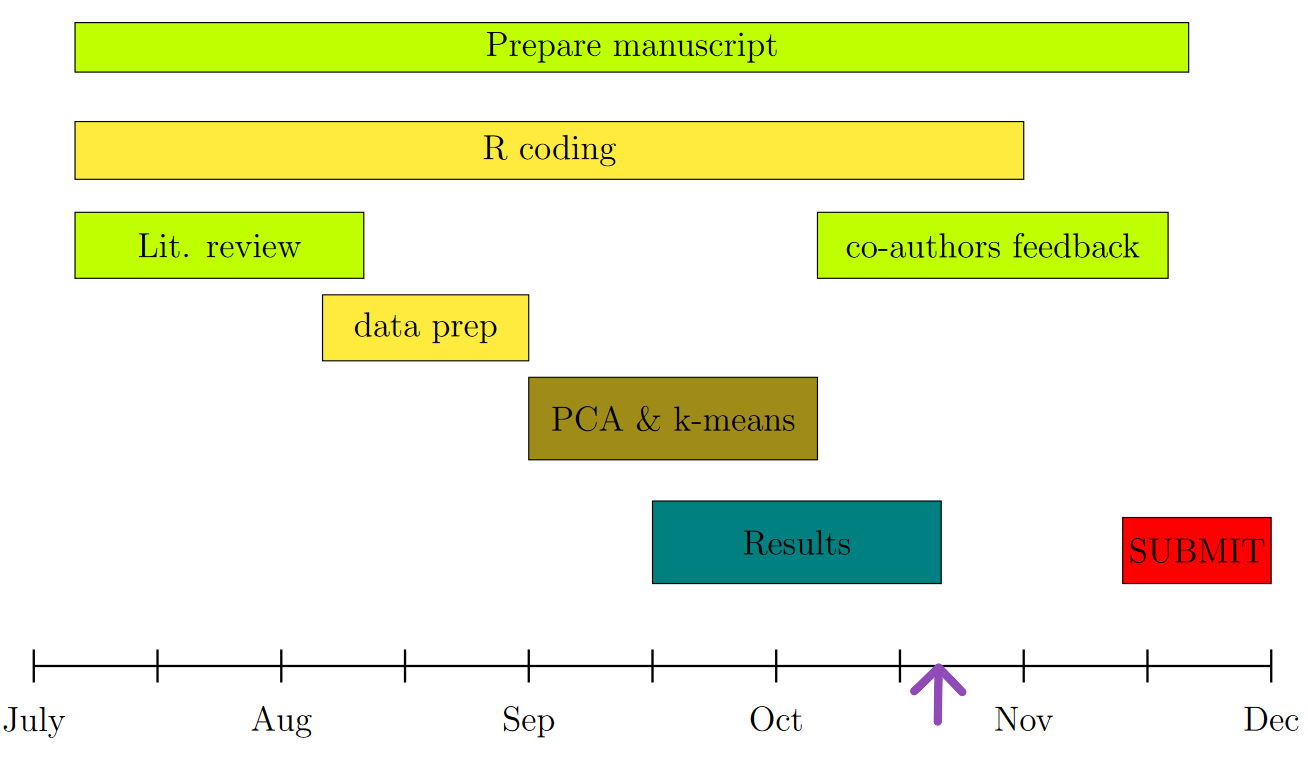
\includegraphics[width=0.6\textwidth,height=\textheight]{imgs/timeline.png}

}

\caption{We are on-time with our timeline}

\end{figure}

\hypertarget{thank-you}{%
\section{Thank you}\label{thank-you}}

\begin{itemize}
\tightlist
\item
  NIA 5R01AG072634-03: Contribution of Longitudinal Neighborhood
  Determinants to Cognitive Health and Dementia Disparities within a
  Multi-Ethnic Cohort.
\item
  Y. Michael, A. Auchincloss, T. McAlexander, S. Melley, K. Moore, B.
  Sánchez, S. Francisco and \textbf{J. Hirsch}
\end{itemize}



\end{document}
